%%%%%%%%%%%%%%%%%%%%%%% file template.tex %%%%%%%%%%%%%%%%%%%%%%%%%
%
% This is a general template file for the LaTeX package SVJour3
% for Springer journals.          Springer Heidelberg 2010/09/16
%
% Copy it to a new file with a new name and use it as the basis
% for your article. Delete % signs as needed.
%
% This template includes a few options for different layouts and
% content for various journals. Please consult a previous issue of
% your journal as needed.
%
%%%%%%%%%%%%%%%%%%%%%%%%%%%%%%%%%%%%%%%%%%%%%%%%%%%%%%%%%%%%%%%%%%%
%
% First comes an example EPS file -- just ignore it and
% proceed on the \documentclass line
% your LaTeX will extract the file if required
\begin{filecontents*}{example.eps}
%!PS-Adobe-3.0 EPSF-3.0
%%BoundingBox: 19 19 221 221
%%CreationDate: Mon Sep 29 1997
%%Creator: programmed by hand (JK)
%%EndComments
gsave
newpath
  20 20 moveto
  20 220 lineto
  220 220 lineto
  220 20 lineto
closepath
2 setlinewidth
gsave
  .4 setgray fill
grestore
stroke
grestore
\end{filecontents*}
%
\RequirePackage{fix-cm}
%
\documentclass{svjour3}                     % onecolumn (standard format)
%\documentclass[smallcondensed]{svjour3}     % onecolumn (ditto)
%\documentclass[smallextended]{svjour3}       % onecolumn (second format)
%\documentclass[twocolumn,draft]{svjour3}          % twocolumn
%
\smartqed  % flush right qed marks, e.g. at end of proof
%
\usepackage{graphicx}
\usepackage{url}
\usepackage{microtype}
%
% \usepackage{mathptmx}      % use Times fonts if available on your TeX system
%
% insert here the call for the packages your document requires
%\usepackage{latexsym}
% etc.
%
% please place your own definitions here and don't use \def but
% \newcommand{}{}
%
% Insert the name of "your journal" with
% \journalname{myjournal}
%
\begin{document}

\journalname{Empirical Software Engineering}

\title{AI-Assisted Programming in Software Engineering}
\subtitle{A Systematic Literature Review and Socio-Technical Perspective}

\titlerunning{AI Assisted Programming in SE}        % if too long for running head

\author{León Felipe Guevara-Chávez}

%\authorrunning{Short form of author list} % if too long for running head

\institute{León Felipe Guevara-Chávez \at
              School of Engineering and Science \\
              Tecnológico de Monterrey \\
%              Tel.: +123-45-678910\\
  %            Fax: +123-45-678910\\
              \email{leon.guevara@tec.mx}           %  \\
%             \emph{Present address:} of F. Author  %  if needed
}

\date{Received: date / Accepted: date}
% The correct dates will be entered by the editor


\maketitle

\begin{abstract}
The rapid integration of large language model (LLM)-based coding assistants into software development practice has generated a substantial but fragmented empirical record. Individual studies report measurable productivity gains alongside increased technical debt, security vulnerabilities, and verification overhead, yet no integrative account has explained why gains in one dimension so consistently coincide with costs in another. This paper presents a systematic literature review of 312 empirical studies on AI-assisted programming published between 2021 and 2026, synthesised across seven analytical dimensions: productivity, code quality and technical debt, human--AI interaction, cognitive load, organisational impact, economic impact, and perception and trust. Following PRISMA 2020 and Kitchenham protocols, studies were identified through a dual-pathway search strategy combining AI-assisted discovery with author-executed database queries, and classified by methodological rigour using a structured quality-assessment framework.

The synthesis shows that AI-assisted programming reliably accelerates code generation but does not by itself reduce total development effort: verification overhead, coordination cost, and cognitive redistribution systematically absorb a substantial share of the time saved in generation. These patterns are formalised as a socio-technical equilibrium framework comprising five interacting constructs: generation efficiency, verification overhead, interaction quality, trust calibration, and cognitive redistribution. The framework is derived inductively from the evidence and tested against the corpus's own internal contradictions and against rival theoretical readings.

Key findings include: productivity gains concentrate in routine, well-specified tasks and diminish or reverse as complexity and contextual dependencies increase; between 33\% and 49\% of AI-generated code contains security vulnerabilities in comparative evaluations, with developer confidence tracking risk inversely in the most controlled studies; interaction quality and prompting and validation literacy emerge as primary conditioning factors of performance variability, functioning as professional competencies distinct from general programming skill; and multi-agent configurations, despite higher autonomy, do not outperform single-agent approaches on most evaluated tasks, suggesting that increasing automation raises coordination and governance demands rather than eliminating them. Economic evidence remains the thinnest dimension in the corpus, with the trade-off between generation efficiency and validation cost still unresolved at the system level.

The socio-technical equilibrium perspective advanced here reframes AI-assisted programming not as a productivity enhancer with side effects, but as a reconfiguration of where development effort is concentrated, who bears it, and whether that reconfiguration is governed or left to accumulate as unrecorded cost. Implications for practice, governance, and future research design are discussed.

\keywords{AI-assisted programming \and Systematic literature review \and Socio-technical equilibrium \and Code quality \and Human–AI collaboration \and Developer productivity}
% \PACS{PACS code1 \and PACS code2 \and more}
% \subclass{MSC code1 \and MSC code2 \and more}
\end{abstract}

% Introduction starts here
\section{Introduction}
\label{intro}

Large language model (LLM)-based coding assistants, including GitHub Copilot, ChatGPT, Claude Code, and an increasingly autonomous generation of coding agents, have moved from experimental tooling to standard development infrastructure in many leading technology organisations in a remarkably short period. Adoption figures illustrate the scale of this shift: one large-scale enterprise deployment reports 16,000 developers using an AI-assisted coding system in production, with roughly a fifth of suggestions accepted and a measurable share of committed code AI-authored \cite{murali_ai-assisted_2024}, while broader developer surveys report usage rates above 80\% among respondents \cite{sergeyuk_using_2025}. AI-assisted programming is therefore no longer a question of whether it will be adopted, but of what its adoption is actually doing to software development practice.

The empirical record on that second question is considerably less settled than the adoption figures suggest. Individual studies report substantial productivity gains, particularly on routine and well-specified tasks, alongside a parallel and growing body of evidence documenting increased technical debt, security vulnerabilities, validation overhead, and, in at least one controlled field experiment, a net productivity loss for experienced developers despite their own belief that the tool had made them faster \cite{becker_measuring_2025}. Reports of high developer satisfaction coexist with evidence that a large share of nominal time savings is absorbed by checking, correcting, and integrating generated code rather than eliminated outright. Taken individually, none of these findings is surprising; taken together, across productivity, code quality, human--AI interaction, cognitive load, organisational impact, economic impact, and developer perception, they describe a literature that is accumulating evidence faster than it is accumulating an explanation for why that evidence so often points in different directions at once.

Several prior reviews have already mapped parts of this terrain. Broad surveys of large language models for software engineering and code generation have catalogued model capabilities, benchmark performance, and technical evaluation methodology at scale \cite{hou_large_2023,zhang_survey_2023,jabrw_systematic_2025,chen_survey_2024}, while narrower systematic reviews have synthesised evidence within a single dimension, including code accuracy, security, and developer trust \cite{naaz_rise_2025}, human--AI interaction within integrated development environments specifically \cite{sergeyuk_human-ai_2026}, and early productivity evidence for a single tool \cite{adepoju_github_2023}. These reviews have been essential in establishing what is technically possible and in consolidating evidence within their respective scopes. What remains absent is a synthesis that treats the technical, human, organisational, and economic dimensions of AI-assisted programming as parts of a single interacting system rather than as separately reviewed literatures, and that offers an explanatory account of why gains in one dimension so consistently coincide with costs in another, rather than simply cataloguing both as separate findings.

This study addresses that gap. It presents a systematic literature review of empirical research on AI-assisted programming published between 2021 and 2026, following PRISMA 2020 reporting guidelines \cite{page_prisma_2021} and established evidence-based software engineering review practice \cite{kitchenham_guidelines_2007}. The review synthesises 312 primary empirical studies, identified through a dual-pathway search strategy combining AI-assisted discovery with author-executed database queries, and organised across seven analytical dimensions: productivity, code quality and technical debt, human--AI interaction, cognitive load, organisational impact, economic impact, and perception and trust. Rather than treating these dimensions as independent literatures to be summarised in parallel, this review integrates them through a socio-technical equilibrium framework comprising five interacting constructs, generation efficiency, verification overhead, interaction quality, trust calibration, and cognitive redistribution, that is developed inductively from the evidence itself and then tested against the corpus's own internal points of agreement and disagreement.

The review is guided by a single research question:

\begin{itemize}
    \item RQ1: What is the impact of AI-assisted programming on software development processes and outcomes?
\end{itemize}

This study makes the following contributions:

\begin{itemize}
    \item A systematic synthesis of 312 empirical studies on AI-assisted programming across seven analytical dimensions, substantially larger in scope than prior reviews in this space and grounded in full-text evidence extraction rather than title-and-abstract coding alone.
    \item A socio-technical equilibrium framework, comprising five interacting constructs, that explains recurring contradictions in the literature as patterned trade-offs rather than as noise, and that is explicitly tested against rival theoretical readings of the same evidence.
    \item Identification of prompting and validation literacy as an emerging professional competency, distinct from general programming skill, that measurably conditions whether AI assistance translates into reliable engineering outcomes.
    \item An explicit mapping of where the corpus agrees and where it does not, showing that disagreement tracks what is measured, snippet-level, repository-level, single-agent, or multi-agent, rather than whether AI assistance helps or hurts in the abstract.
    \item A research agenda grounded in the evidence gaps this review identifies directly, including the thinness of economic-impact evidence, the immaturity of agentic and multi-agent evaluation, and the uneven distribution of cognitive redistribution across developer populations.
\end{itemize}

The remainder of this paper is organised as follows. Section~\ref{sec:methodology} describes the review methodology, including the search strategy, quality assessment framework, and use of AI-assisted tools in the review process. Section~\ref{sec:results} presents the empirical results across all seven analytical dimensions. Section~\ref{sec:discussion} discusses these results through the socio-technical equilibrium framework and tests that framework against the corpus's internal disagreements and against rival theoretical readings. Section~\ref{sec:threats} discusses threats to validity, and Section~\ref{conclusion} concludes with implications for research and practice.
% Introduction ends here

% Methodology start here
\section{Methodology}
\label{sec:methodology}

\subsection{Research Design}
\label{sec:research-design}
This study follows a Systematic Literature Review (SLR) methodology, structured according to established evidence-based software engineering guidelines \cite{kitchenham_guidelines_2007} and the PRISMA 2020 framework \cite{page_prisma_2021} to ensure transparency, rigour, and reproducibility.

The objective is to identify, evaluate, and synthesise empirical evidence regarding the impact of AI-assisted programming tools on software development. The review process was designed as a multi-stage protocol comprising two complementary discovery pathways, screening, eligibility assessment, quality evaluation, epistemic segmentation, and synthesis.

\subsection{Research Question}
\label{sec:research-question}
The study is guided by the following research question:

\begin{itemize}
    \item RQ1: What is the impact of AI-assisted programming on software development processes and outcomes?
\end{itemize}

To address this question, the analysis was structured across seven analytical dimensions: productivity, code quality and technical debt, human--AI interaction, cognitive load, organisational impact, economic impact, and perception and trust.

\subsection{Search Strategy}
\label{sec:search-strategy}
The literature search combined two complementary discovery pathways. The primary pathway (Branch A) used SciSpace, an AI-assisted academic discovery engine that orchestrates retrieval across multiple indexed sources. The complementary pathway (Branch B) used author-executed direct queries on three academic databases: Scopus, ProQuest, and arXiv. Both pathways targeted publications between 2021 and 2026, reflecting the emergence and rapid evolution of modern AI-assisted coding tools. Bibliographic information for individual papers was occasionally imported from publisher sites (IEEE Xplore, ACM Digital Library, SpringerLink, ACL Anthology); these channels served solely as bibliographic-import mechanisms and are not counted as search sources, since the discovery of each such paper had already occurred on one of the four search sources above.

\subsubsection{Branch A: SciSpace AI-assisted retrieval}
\label{sec:branch-a}
A structured search instruction was provided to SciSpace specifying the review topic, research questions, the time window, inclusion and exclusion criteria, required output fields, and quality-control constraints. SciSpace executed the instruction across three internal retrieval modes: (i) SciSpace Deep Search (855 records from two semantic queries: 371 and 484), (ii) SciSpace Full-Text Search (200 records from two queries of 100 each), and (iii) Google Scholar, queried programmatically by SciSpace as part of its retrieval pipeline (200 records from two queries of 100 each). The combined identification yielded 1,255 records, reduced to 863 unique records after SciSpace's internal deduplication. These records were then carried through SciSpace's two-stage screening pipeline (title/abstract scoring with a cutoff of 4.0, followed by full-text scoring with a cutoff of 4.5), with each AI-assisted decision validated manually by the author against the eligibility criteria described in Section~\ref{sec:inclusion-exclusion}. This branch retained 355 records at title/abstract screening and 349 records at full-text screening. The complete archive of SciSpace's search outputs (query logs, retrieved record CSVs, and screening artefacts) is preserved as supplementary material.

\subsubsection{Branch B: Author-executed database queries}
\label{sec:branch-b}
The author-executed database pathway returned 1,852 records across three sources: 1,713 from Scopus (one export, dated 5 April 2026), 89 from ProQuest (two exports, dated 3 and 5 April 2026), and 50 records browsed on arXiv through a structured keyword search combining AI-assisted-programming, software-engineering, and outcome-related terms (arXiv displays 50 records per result page; the search yielded a single page of results relevant to the review scope). After title/abstract screening (113 retained) and full-text assessment (107 retained), cross-branch deduplication against the SciSpace branch removed 32 duplicate records, yielding a net contribution of 69 unique records. Search strings, filters, and export timestamps for each query are preserved in the supplementary materials of the project. Full query strings and field restrictions are documented in Supplementary Material S2.

\subsection{Use of Artificial Intelligence in the Review Process}
\label{sec:ai-use}
Artificial intelligence tools were used to support specific tasks in the review process. SciSpace functioned as an AI-assisted discovery engine, orchestrating queries across its proprietary semantic indexes, full-text search, and Google Scholar, and as a first-pass relevance scorer for title/abstract and full-text screening. Decisions emitted by SciSpace were treated strictly as assistive recommendations: every inclusion, exclusion, classification, and quality-assessment decision was validated and recorded manually by the author. In addition, the corpus includes a small number of studies published in Chinese, Russian, and German; for these, AI-assisted translation (ChatGPT) was used to support the author's reading and eligibility assessment, with the same inclusion criteria applied as for studies in English, Spanish, and Portuguese, which the author read directly. Beyond discovery, screening support, and language translation, AI tools supported two additional tasks under explicit safeguards: NotebookLM was used for corpus-wide thematic exploration and initial descriptive characterisation, and ChatGPT (4o/o1 family) was used for single-paper deep extraction of quantitative findings and scaffolding of structured artefacts; Elicit was used in a limited pilot for cross-validation of selected quantitative extractions. In each case, AI-assisted outputs were treated as drafts requiring manual verification: all inclusion, exclusion, classification, synthesis, and interpretation decisions were made and recorded manually by the author, and every quantitative figure cited in this manuscript was verified against the original source PDF prior to inclusion. The failure modes identified during a dedicated pilot validation phase, the safeguards applied, and the resulting error rates are documented in Section~\ref{sec:threats} and in supplementary material S3.

\subsection{Inclusion and Exclusion Criteria}
\label{sec:inclusion-exclusion}
Eligibility criteria were applied identically to both branches and at every screening stage. Studies were included if they reported empirical evaluation (quantitative, qualitative, or mixed-methods) of AI-assisted programming or code generation; evaluated modern AI tools (e.g., Copilot, ChatGPT, Codex, Gemini, Claude Code, CodeWhisperer, Cursor, or comparable systems); reported results allowing analytical interpretation; and were published between 2021 and 2026.
 
Studies were excluded if they were opinion papers without empirical content, focused on unrelated NLP tasks, were duplicates of records already accepted from another source, or fell outside the topical scope of AI-assisted software development. Surveys, systematic literature reviews, and conceptually adjacent works were reclassified to the Related Work or Support set rather than discarded, in order to preserve their contribution to the framing of the synthesis.

\subsection{Operational Taxonomy of Records}
\label{sec:taxonomy}
To maintain a transparent and auditable separation between evidence used for synthesis and evidence used for framing, each retained record was assigned to one of five operational categories, summarised in Table~\ref{tab:taxonomy}.

\begin{table}[h]
\centering
\caption{Operational taxonomy of records}
\label{tab:taxonomy}
\begin{tabular}{l c}
\hline
\textbf{Category} & \textbf{Count ($n$)} \\
\hline
Corpus (primary empirical evidence base) & 312 \\
Related Work or Support & 67 \\
Duplicated & 21 \\
No Full Text & 22 \\
Excluded & 5 \\
\hline
\end{tabular}
\end{table}

The Corpus comprises the primary empirical evidence base: studies with empirical results directly analysed across the seven analytical dimensions, weighted by an epistemic segmentation described below. The Related Work or Support category comprises surveys, systematic reviews, and conceptually adjacent works providing theoretical and contextual grounding; these are cited in the Introduction and Discussion but are not counted in corpus statistics. The Duplicated category preserves preprint/published-version pairs of records already represented in another sheet (internal SciSpace duplicates), retained for audit transparency. The No Full Text category records studies whose full text could not be retrieved, excluded from empirical analysis but retained for traceability. The Excluded category comprises records that entered the structured screening pipeline but failed quality or scope criteria at full-text assessment.

Within the Corpus, a further epistemic segmentation governs interpretive weight: CORE (168 studies), SUPPORTING (120 studies), PERIPHERAL (18 studies), and REMOVE\_CANDIDATE (6 studies). All descriptive statistics reported in this paper are computed over the full Corpus ($n = 312$), while strong claims are preferentially anchored in CORE studies and triangulated with SUPPORTING evidence.

\subsection{Study Selection Process and PRISMA Flow}
\label{sec:prisma-flow}
The selection process followed the four-phase PRISMA 2020 framework (Identification, Screening, Eligibility, Inclusion) and was applied to both branches in parallel, as shown in Fig.~\ref{fig:prisma_diagram}. Although the search targeted publications from 2021, no study meeting the inclusion criteria was identified for that year.

At identification, the SciSpace pipeline (Branch A) returned 1,255 records, reduced to 863 unique records after its internal deduplication; the author-executed database pathway (Branch B) returned 1,852 records across Scopus, ProQuest, and arXiv. At title/abstract screening, 355 records were retained from Branch A and 113 from Branch B. At full-text screening, 349 records were retained from Branch A and 107 from Branch B. Cross-branch deduplication then removed 32 Branch B records that duplicated SciSpace hits, yielding a net Branch B contribution of 69 records.

The two branches thus converged into an integrated dataset of 418 unique records from structured search (349 from Branch A and 69 net from Branch B). This dataset was subjected to manual quality refinement and dimensional classification, and distributed across the five operational sheets defined in Section~\ref{sec:taxonomy}, yielding 308 records for the Corpus and 62 for Related Work or Support (together with 21 Duplicated, 22 No Full Text, and 5 Excluded records, totalling 418).

A supplementary discovery procedure was then applied selectively to address residual gaps and to preserve methodological transparency. This procedure covered three situations: (i) targeted keyword search prompted by gap diagnosis when a specific analytical dimension showed insufficient empirical depth; (ii) citation chasing from references in already-retrieved papers; and (iii) opportunistic retrieval during full-text resolution, including cases where related-link panels or alternative result lists surfaced conceptually relevant works. All candidates identified through this procedure were subjected to the same eligibility criteria and quality-assessment framework as papers retrieved through the two structured pathways.

This supplementary procedure added four primary studies to the Corpus (4 of 312, or 1.3\%) and five additional studies to Related Work or Support (5 of 67, or 7.5\%), bringing the final totals to 312 and 67 respectively. One foundational study published in 2020 (Brachten et al., on cognitive-load reduction by virtual agents) was retained explicitly as a Related Work reference, providing the conceptual basis for the cognitive-load--performance relationship subsequently extended by the field toward AI-assisted coding tools; it is not counted in the empirical corpus statistics. The full audit trail for the nine supplementary records, including provenance and discovery type, is provided in the supplementary materials.

\begin{figure}[h]
    \centering
    
\includegraphics[width=0.9\linewidth]{figures/prisma_diagram.png}
    \caption{PRISMA 2020 dual-pathway flow diagram for the systematic literature review.}
    \label{fig:prisma_diagram}
\end{figure}

\subsection{Quality Assessment}
\label{sec:quality-assessment}
A multi-criteria evaluation framework was used to assess study quality, considering empirical rigour (e.g., experimental design, sample size), methodological strength (e.g., causal inference versus observational design), venue quality, completeness and transparency of reporting, and relevance to the research question. This framework was applied consistently across all studies to ensure comparability and reduce subjective bias, and was conducted manually to ensure careful evaluation of study design and reporting quality.

Studies were classified into three categories: A1 (high rigour, e.g., controlled experiments or large-scale empirical or causal studies), A2 (moderate rigour, e.g., user studies, case studies, or structured evaluations), and B (supporting evidence, e.g., perception studies, qualitative analyses, or model-based approaches). Of the 312 studies in the Corpus, 146 (46.8\%) were classified as A1, 132 (42.3\%) as A2, and 34 (10.9\%) as B. This classification was used to prioritise higher-quality studies (A1 and A2) in the synthesis and interpretation of results, while category B studies were primarily used to provide contextual support and complementary insights.

\subsection{Data Extraction and Synthesis}
\label{sec:data-extraction}
Data extraction was performed by systematically reviewing each selected study and recording key attributes using a structured extraction template to ensure consistency across studies. For each study, the following data were extracted: study type and methodological classification, tools evaluated, evaluation metrics, key findings, and associated analytical dimensions.

Given the heterogeneity of study designs, metrics, and evaluation contexts, a formal meta-analysis was not feasible. Instead, a structured synthesis approach was adopted to identify consistent patterns and trends across studies, combining quantitative aggregation (e.g., frequency distributions) with qualitative synthesis to identify patterns, contradictions, and research gaps across dimensions. This approach is consistent with established practices in systematic literature reviews, where high variability limits the applicability of statistical meta-analysis.

\subsection{Reproducibility and Sensitivity}
\label{sec:reproducibility}
All search exports and the integrated relation of studies are preserved as supplementary materials, including SciSpace's complete pipeline artefacts (semantic-search CSVs, full-text-search CSVs, internally executed Google Scholar query CSVs, abstract- and full-text-screening CSVs, and SciSpace's own PRISMA documentation). Of the 312 primary studies in the final Corpus, 308 (98.7\%) are directly traceable to documented structured-search outputs; of the 67 papers in Related Work or Support, 62 (92.5\%) are similarly traceable; and all 5 papers in the Excluded set are traceable to structured queries.

To assess the robustness of the reported figures to the inclusion of the nine supplementary-discovery records, a sensitivity analysis was conducted by recomputing all principal distributions (primary dimension, quality classification, epistemic segmentation, and publication year) for the full Corpus ($n = 312$) and for the Corpus with the four supplementary studies removed ($n = 308$). Across all four axes, no reported percentage shifts by more than 0.80 percentage points, with the largest single shift occurring in the 2025 publication-year share. This confirms that the inclusion of supplementary studies does not materially alter the empirical profile of the corpus, and that the principal findings hold whether or not these studies are included.
% Methodology ends here

% Results start here
\section{Results}
\label{sec:results}
% 3.1 starts here
\subsection{Corpus Profile and Evidence Hierarchy}
\label{sec:corpus-profile}
The final corpus comprises 312 studies, reflecting a heterogeneous body of evidence in terms of methodological rigour, evaluation context, and analytical focus. Studies were classified into three quality categories: A1 (high rigour), A2 (moderate rigour), and B (supporting or qualitative evidence).

Of the 312 studies, 146 (46.8\%) were classified as A1, 132 (42.3\%) as A2, and 34 (10.9\%) as B, as shown in Fig.~\ref{fig:main_classification}. This distribution indicates that the majority of the evidence base is grounded in empirical studies with moderate-to-high methodological rigour.

\begin{figure}[h]
    \centering
    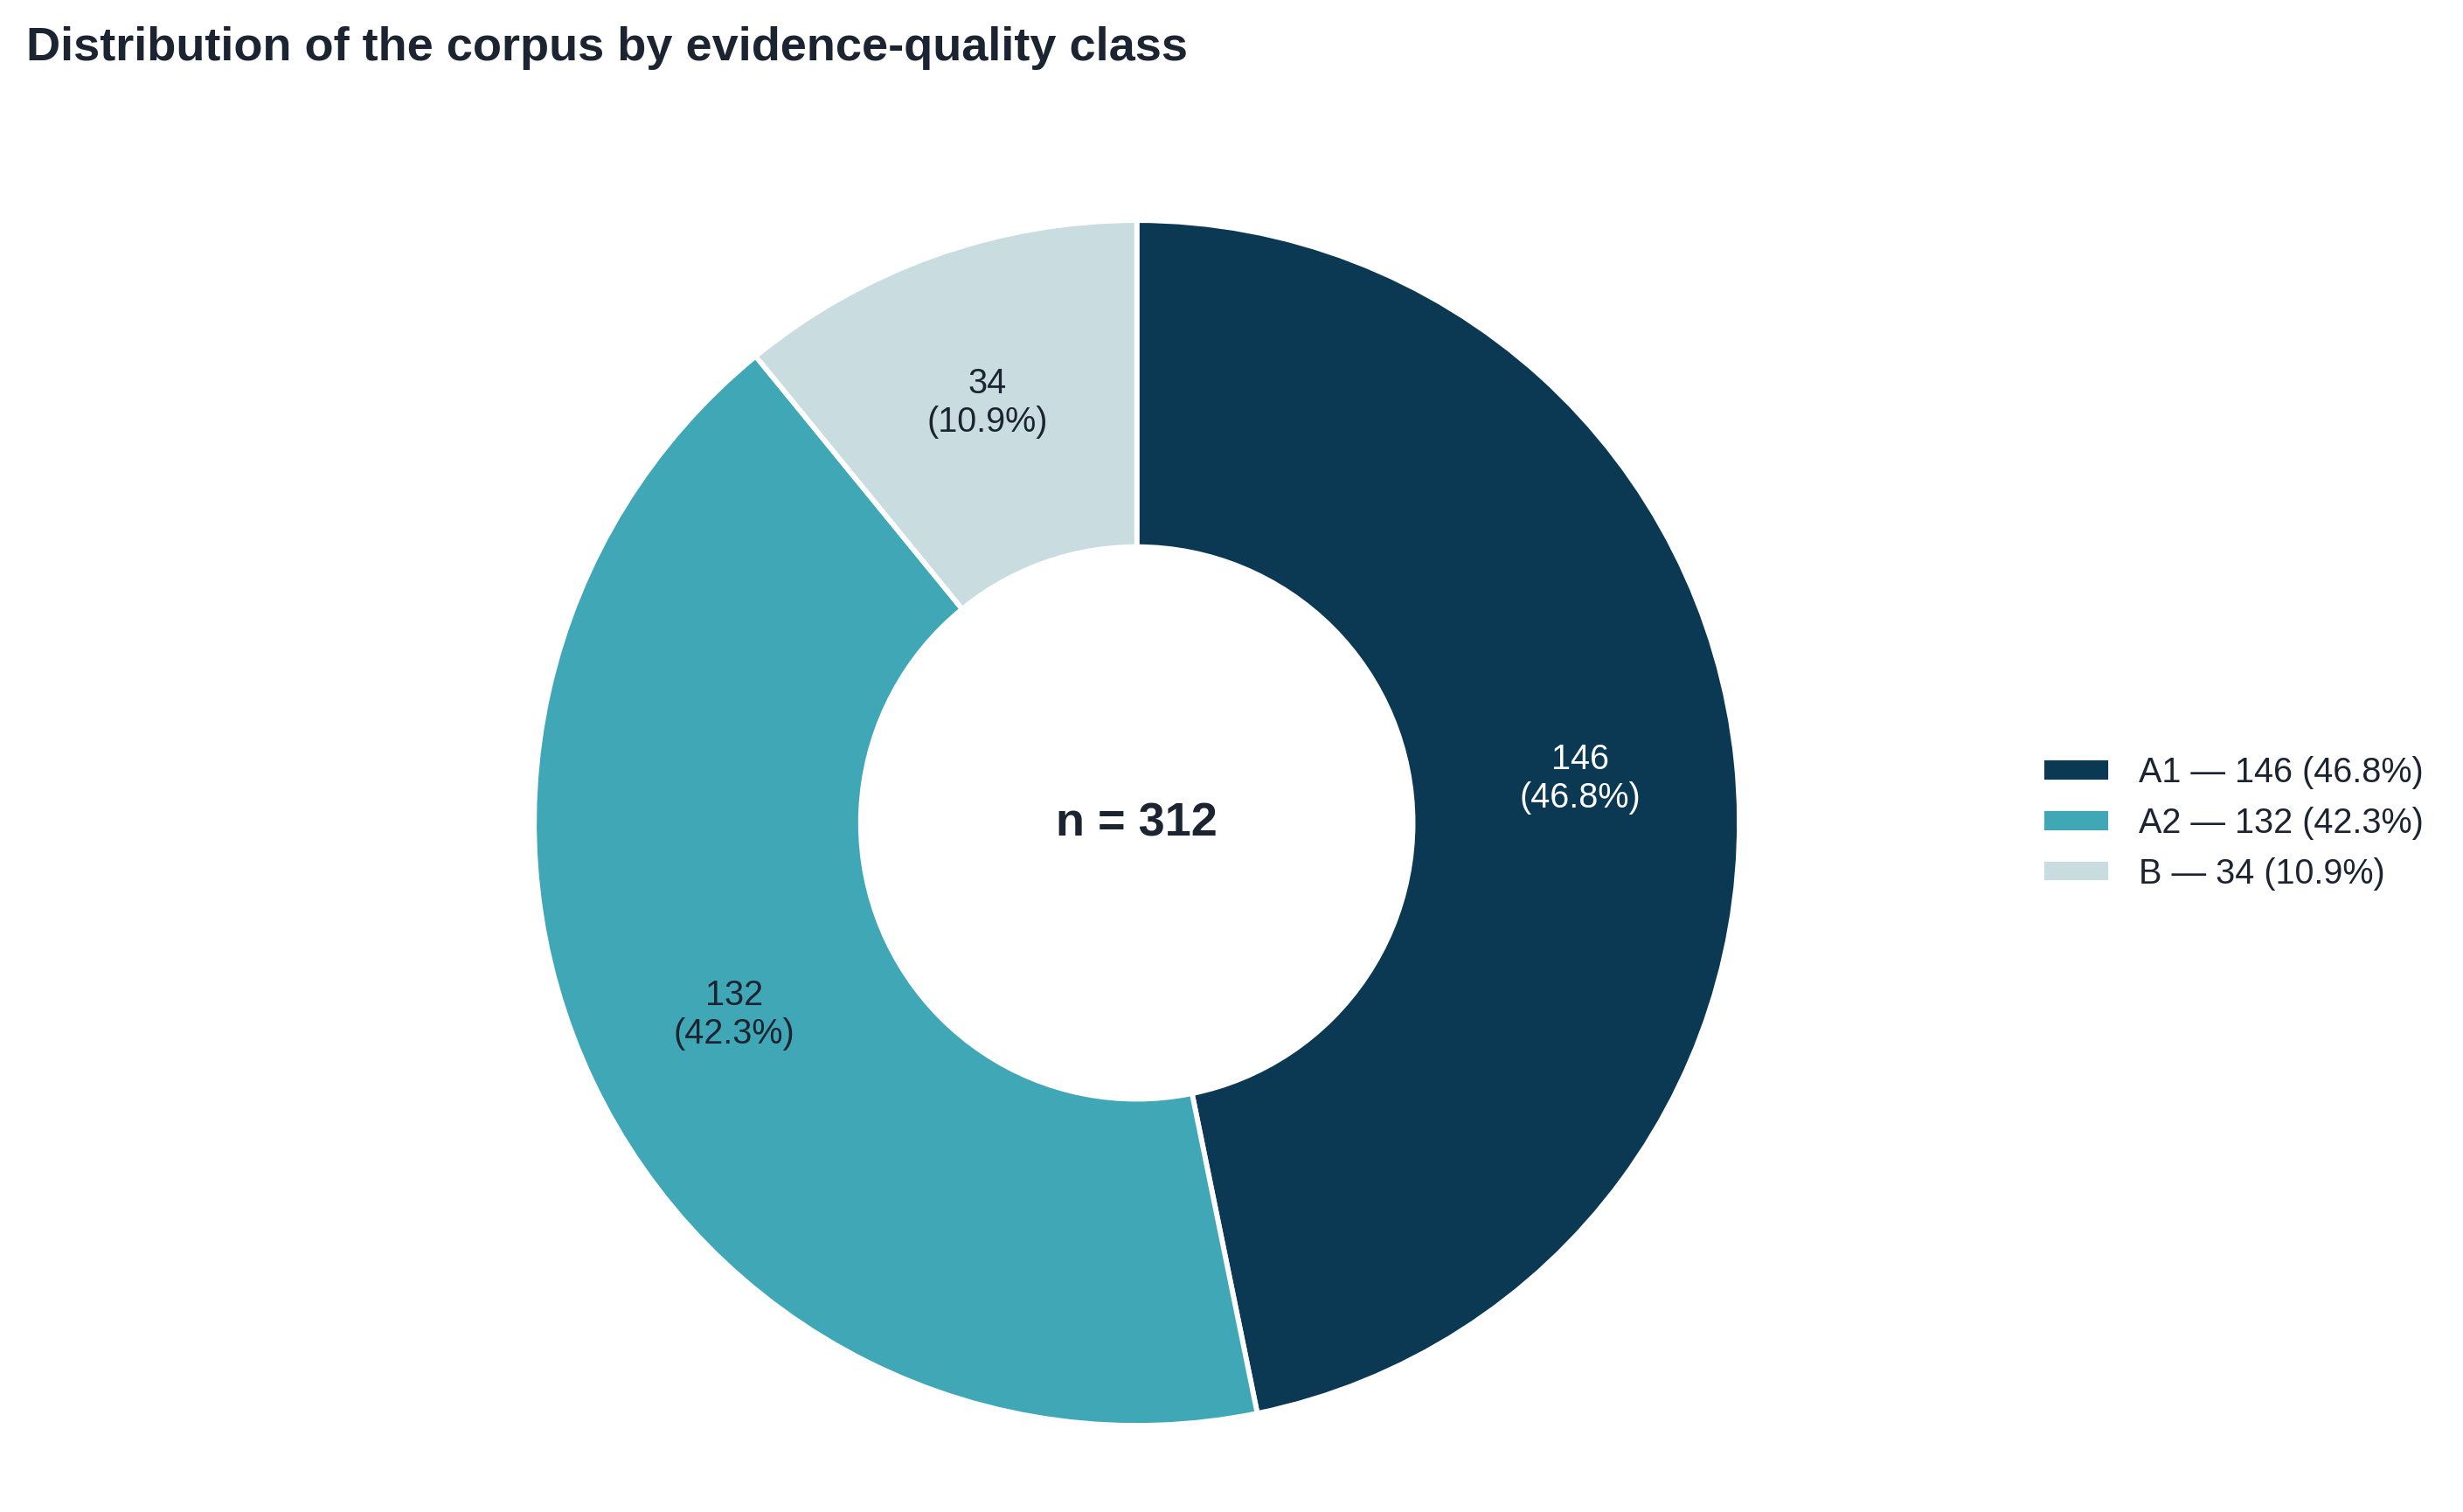
\includegraphics[width=0.82\linewidth]{figures/A2_quality_distribution.png}
    \caption{Distribution of the final corpus by evidence class (A1, A2, and B).}
    \label{fig:main_classification}
\end{figure}

In terms of analytical dimensions, as shown in Fig.~\ref{fig:dimensions}, the corpus is markedly concentrated in two areas: code quality and technical debt accounts for 45.2\% of studies (n=141), and human--AI interaction for a further 36.9\% (n=115). Together, these two dimensions represent more than four-fifths of the corpus. The remaining studies are distributed across productivity (8.3\%, n=26), perception and trust (4.2\%, n=13), cognitive load and human factors (2.9\%, n=9), organisational impact (2.2\%, n=7), and economic impact (0.3\%, n=1).

\begin{figure}[h]
    \centering
    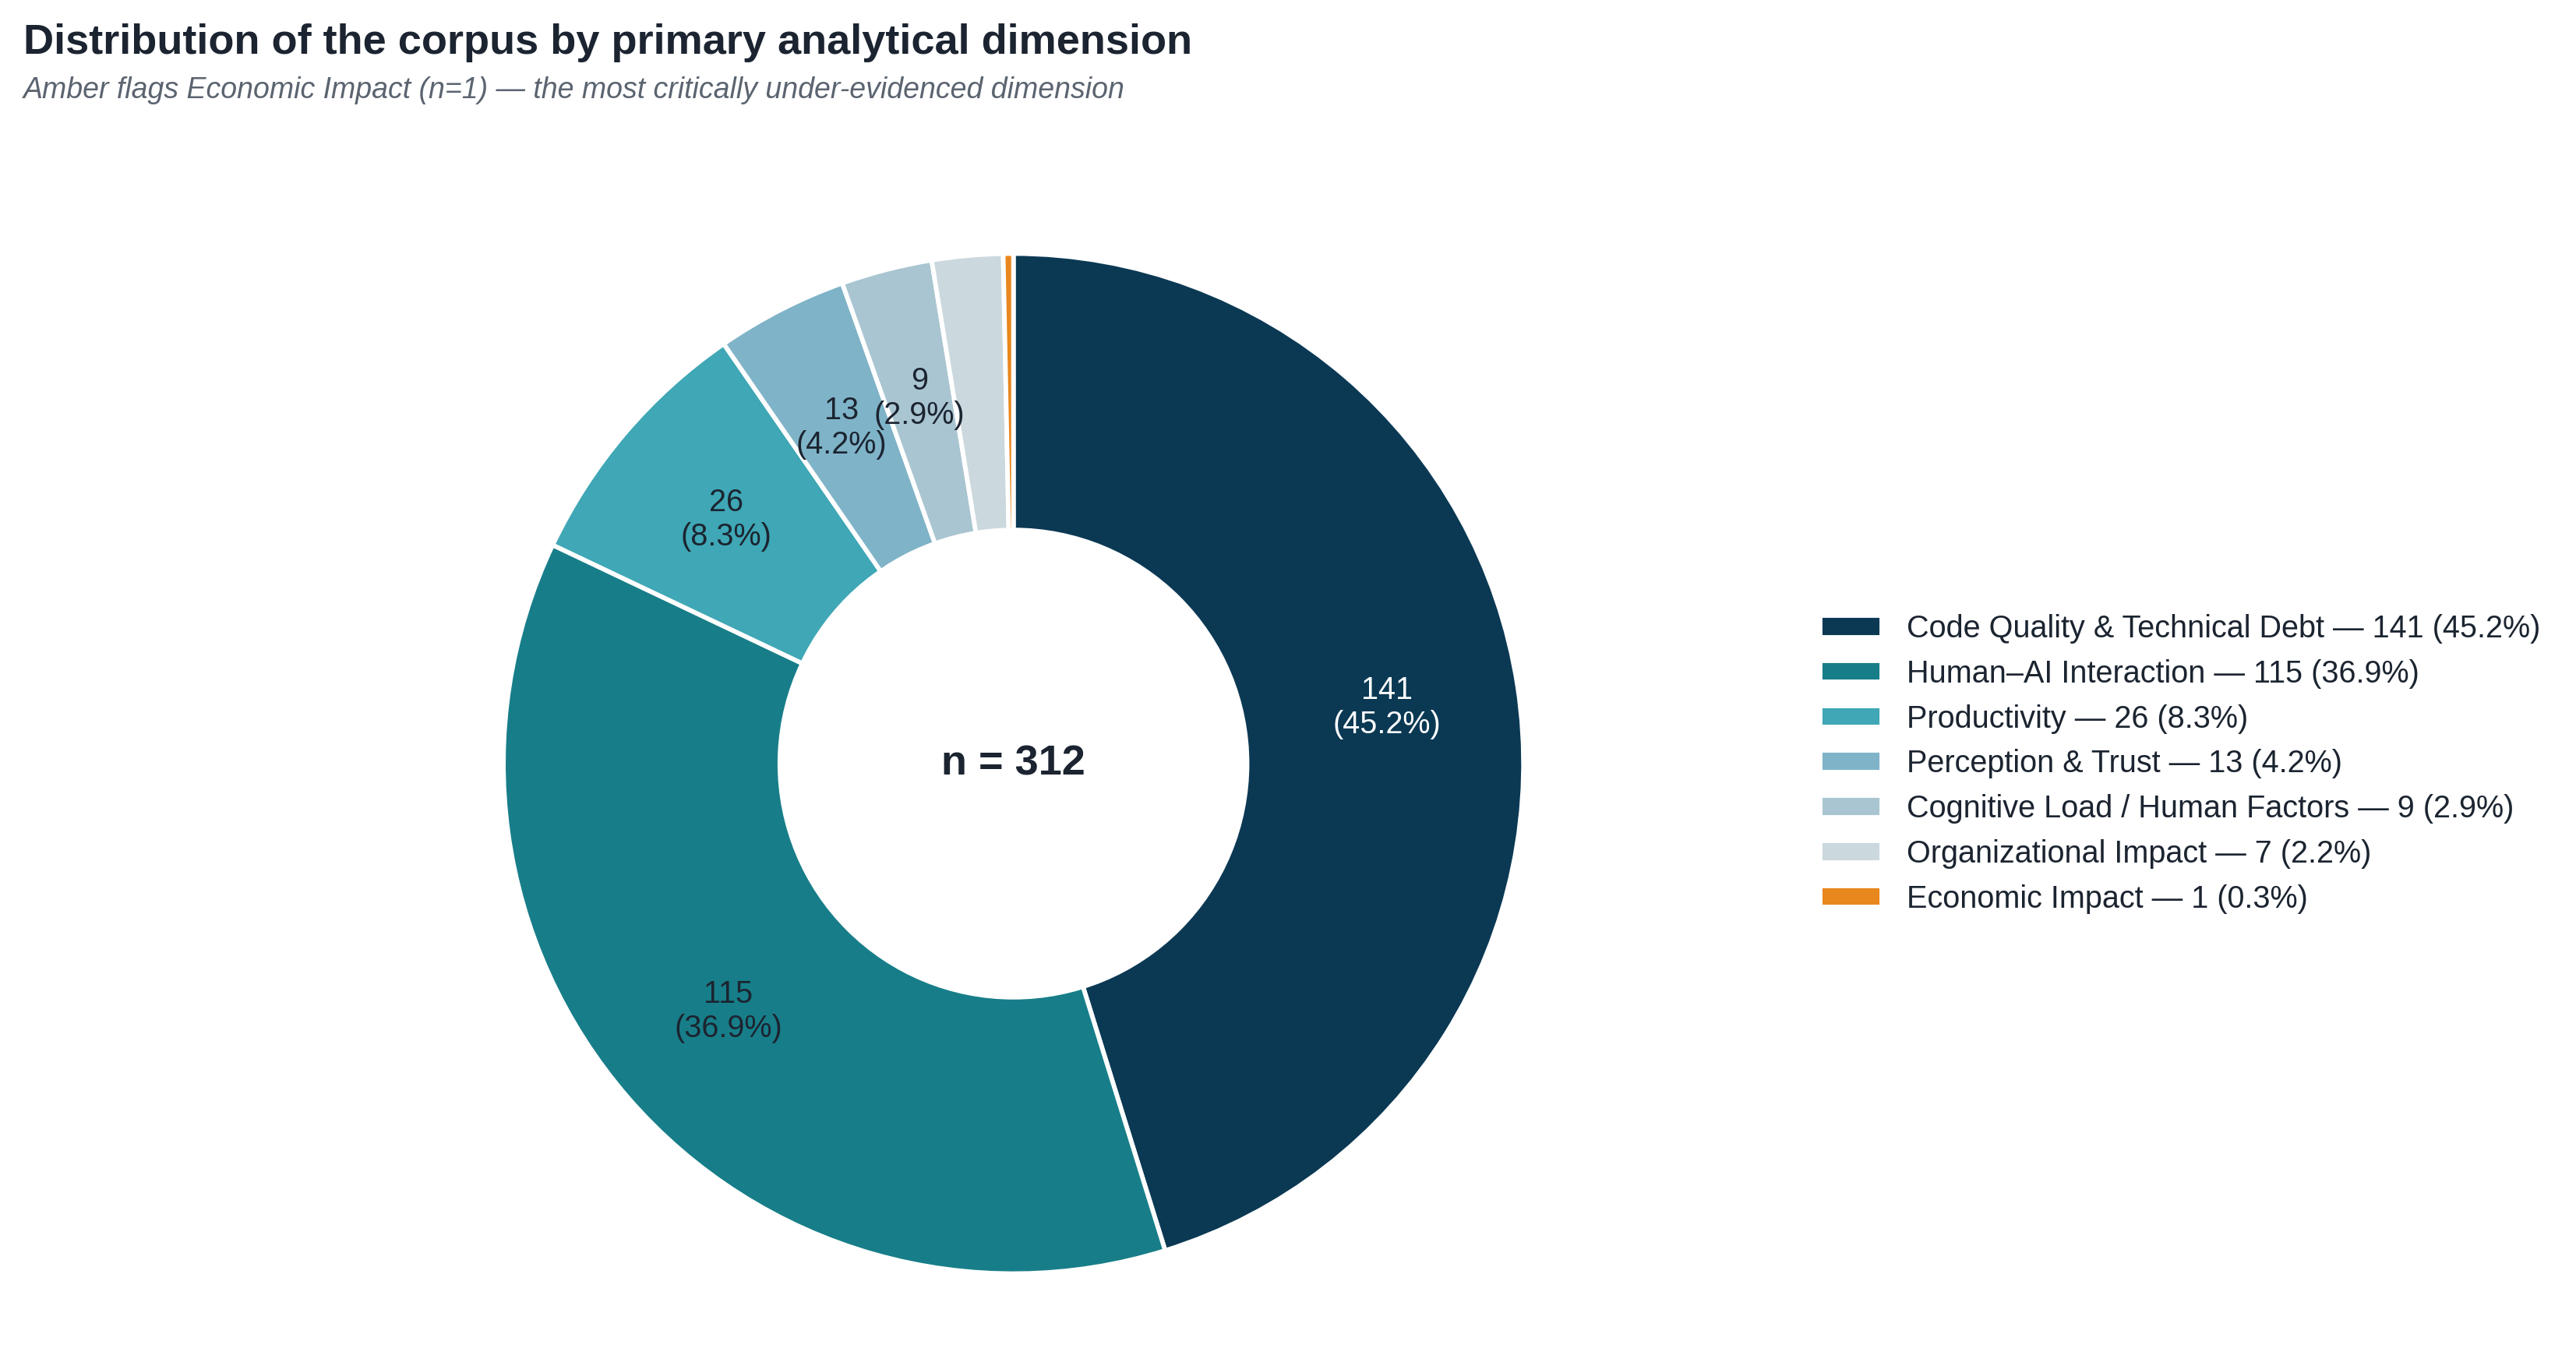
\includegraphics[width=0.82\linewidth]{figures/A1_dimension_distribution.png}
    \caption{Distribution of the corpus across the seven analytical dimensions (primary dimension classification). Amber flags Economic Impact (n=1), the most critically under-evidenced dimension.}
    \label{fig:dimensions}
\end{figure}

This concentration represents a substantial reorientation of the evidence base relative to earlier framings of the literature, which had often emphasised productivity as the dominant research focus. In the present corpus, productivity-focused studies form a comparatively small subset, while the bulk of empirical attention is directed toward the reliability, security, and maintainability of AI-generated code (code quality and technical debt) and toward the iterative, prompt-driven dynamics of developer--AI collaboration (human--AI interaction). Economic impact, organisational impact, and cognitive load remain markedly underexplored, each represented by fewer than ten studies, with economic impact represented by a single study in the corpus.

Quality classification varies systematically across dimensions, as shown in Fig.~\ref{fig:quality_by_dimension}. Code quality and technical debt exhibits the highest concentration of high-rigour evidence, with 55.3\% of its studies classified as A1, reflecting the prevalence of large-scale empirical analyses, controlled benchmarking, and security-focused evaluations in this area. Human--AI interaction shows a more balanced split between A1 and A2 evidence (45.2\% and 44.3\%, respectively), consistent with a mix of large-scale interaction-log studies and smaller controlled or observational user studies. The remaining dimensions are dominated by A2 evidence, with organisational impact showing the highest proportion of category-B studies (42.9\%), reflecting its reliance on qualitative and case-study evidence. Economic impact, the smallest dimension in the corpus, is composed entirely of category-B evidence (100\%), underscoring it as the dimension most in need of methodologically stronger studies.

\begin{figure}[h]
    \centering
    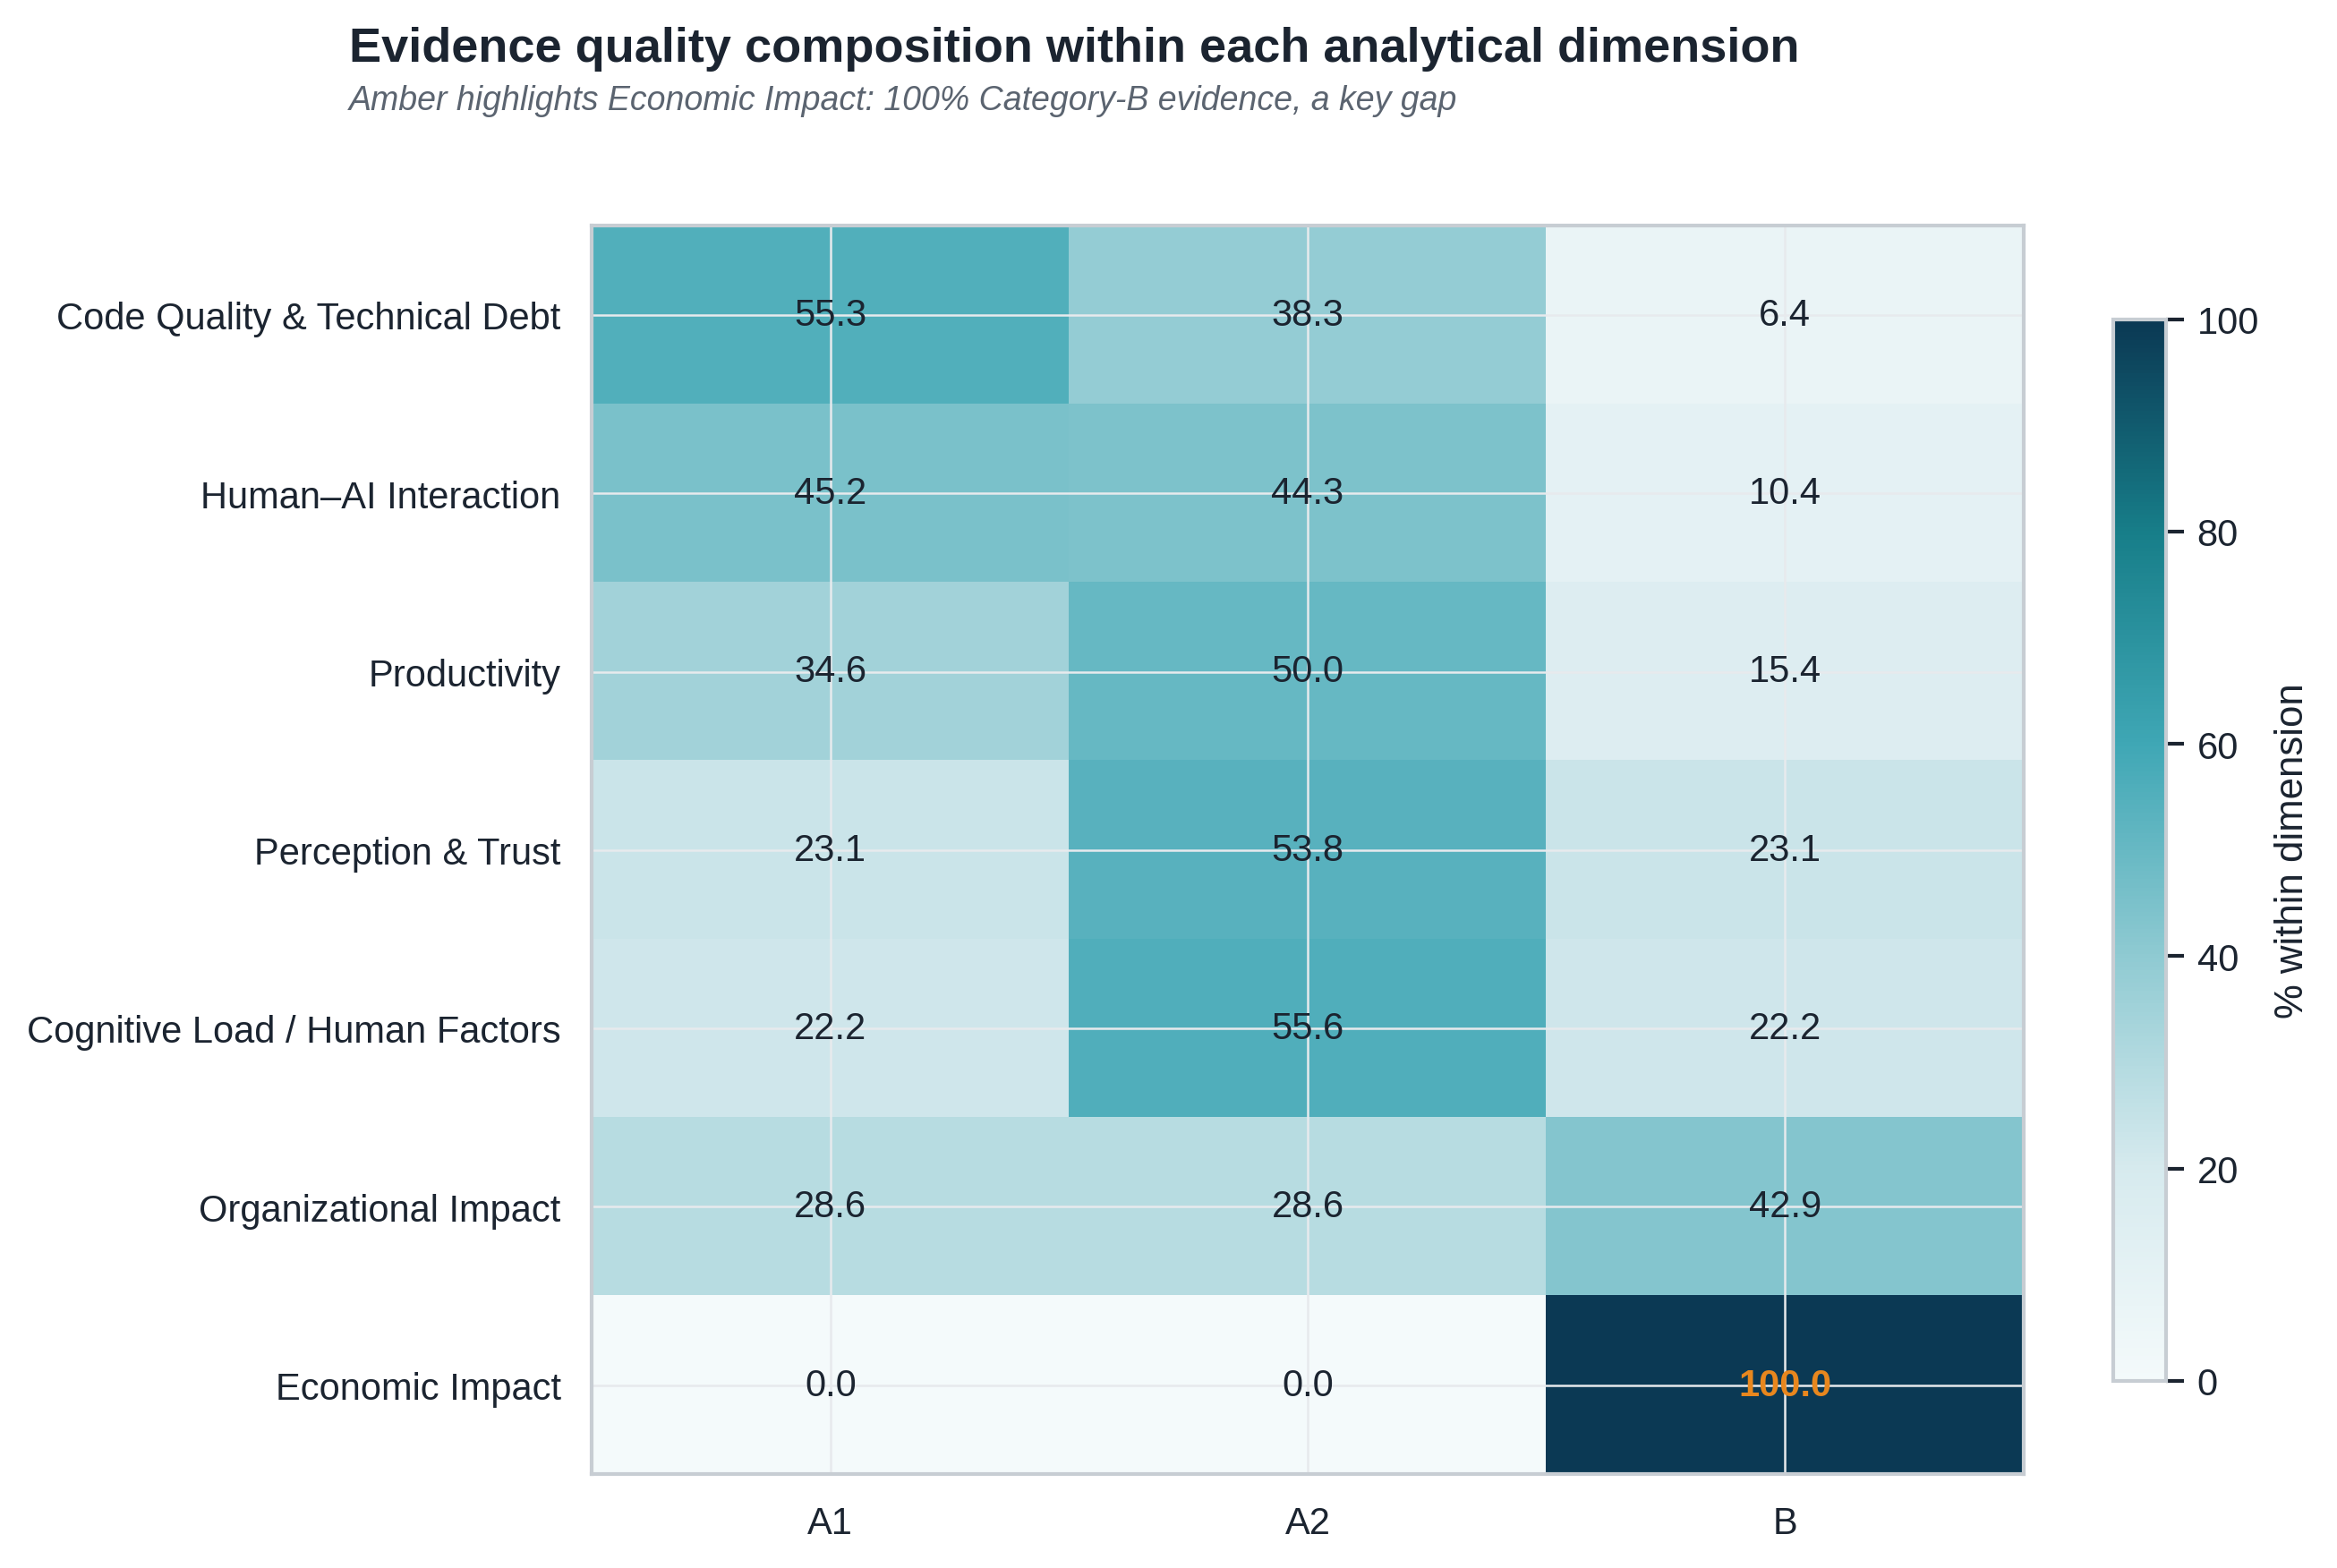
\includegraphics[width=0.82\linewidth]{figures/B1_quality_by_dimension.png}
    \caption{Evidence quality composition within each analytical dimension. Amber highlights Economic Impact: 100\% category-B evidence, a key gap.}
    \label{fig:quality_by_dimension}
\end{figure}

Beyond the primary-dimension classification, an epistemic segmentation was applied to capture the interpretive weight of each study within the synthesis, independently of its analytical dimension. Studies were segmented into CORE (n=168, 53.8\%), SUPPORTING (n=120, 38.5\%), PERIPHERAL (n=18, 5.8\%), and REMOVE\_CANDIDATE (n=6, 1.9\%). CORE studies anchor the principal claims advanced in each dimension; SUPPORTING studies provide corroborating or contextual evidence; PERIPHERAL studies offer tangential but relevant findings; and REMOVE\_CANDIDATE studies, while retained in the corpus for transparency, contribute marginally to the synthesis and are flagged for potential exclusion in future refinements. This segmentation is broadly consistent across dimensions, with code quality and technical debt (77 CORE of 141) and human--AI interaction (60 CORE of 115) each anchoring more than half of their respective dimensions in CORE evidence.

Finally, the corpus spans publications from 2022 to 2026, with a pronounced concentration in the most recent years: 2024 (n=120, 38.5\%) and 2025 (n=121, 38.8\%) together account for more than three-quarters of the corpus, while 2026 already contributes 31 studies (9.9\%) at the time of the search cutoff. Earlier years are represented more sparsely, with 34 studies (10.9\%) from 2023 and 6 studies (1.9\%) from 2022. This temporal distribution reflects the rapid and recent expansion of empirical research on AI-assisted programming, consistent with the accelerating adoption of LLM-based coding tools over the period under review. Fig.~\ref{fig:dimension_by_year} shows how this growth is distributed across dimensions: code quality and technical debt and human--AI interaction account for the bulk of the increase from 2023 onward, while the apparent decline in 2026 reflects the partial-year search cutoff rather than a genuine slowdown in research activity.

\begin{figure}[h]
    \centering
    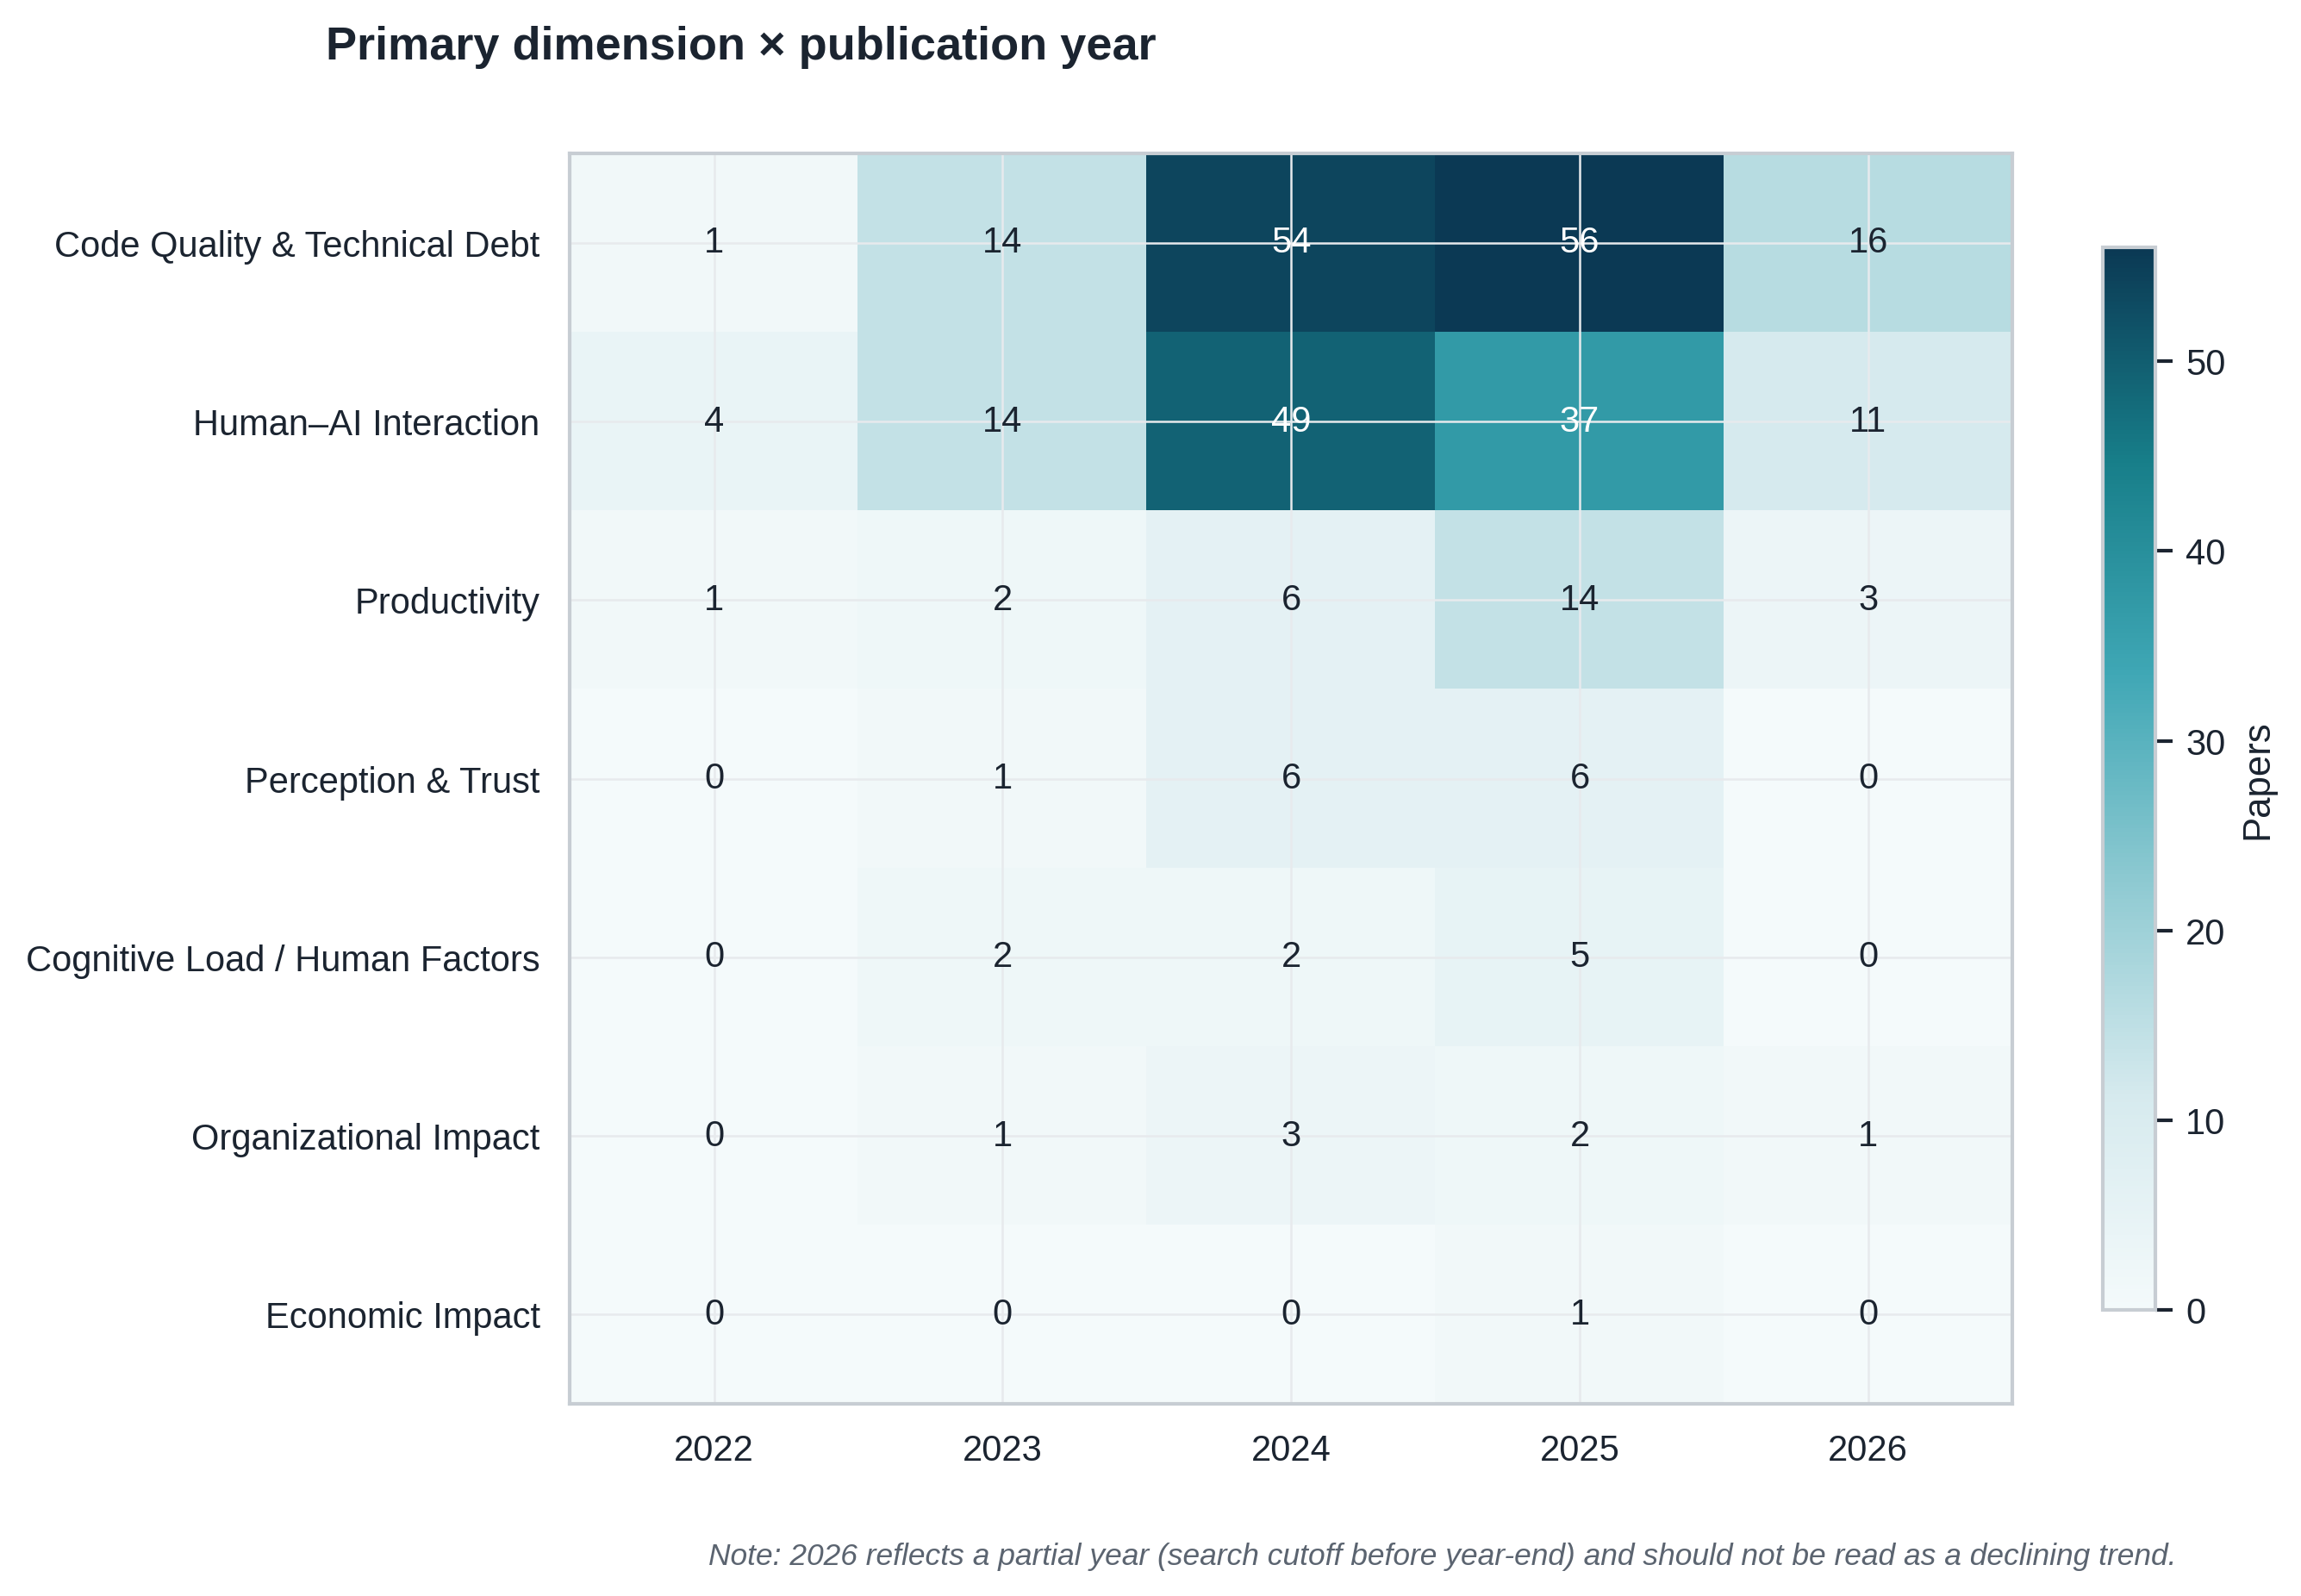
\includegraphics[width=0.82\linewidth]{figures/B2_dimension_by_year.png}
    \caption{Primary dimension by publication year. 2026 reflects a partial year (search cutoff before year-end) and should not be read as a declining trend.}
    \label{fig:dimension_by_year}
\end{figure}

Beyond volume, the methodological rigour of the corpus has also shifted over time. As shown in Fig.~\ref{fig:quality_evolution}, the share of A1 (high-rigour) studies rose from 16.7\% in 2022 to 54.7\% in 2026, indicating that the field is maturing methodologically alongside its rapid growth in volume. This trend is examined further in the Discussion.

\begin{figure}[h]
    \centering
    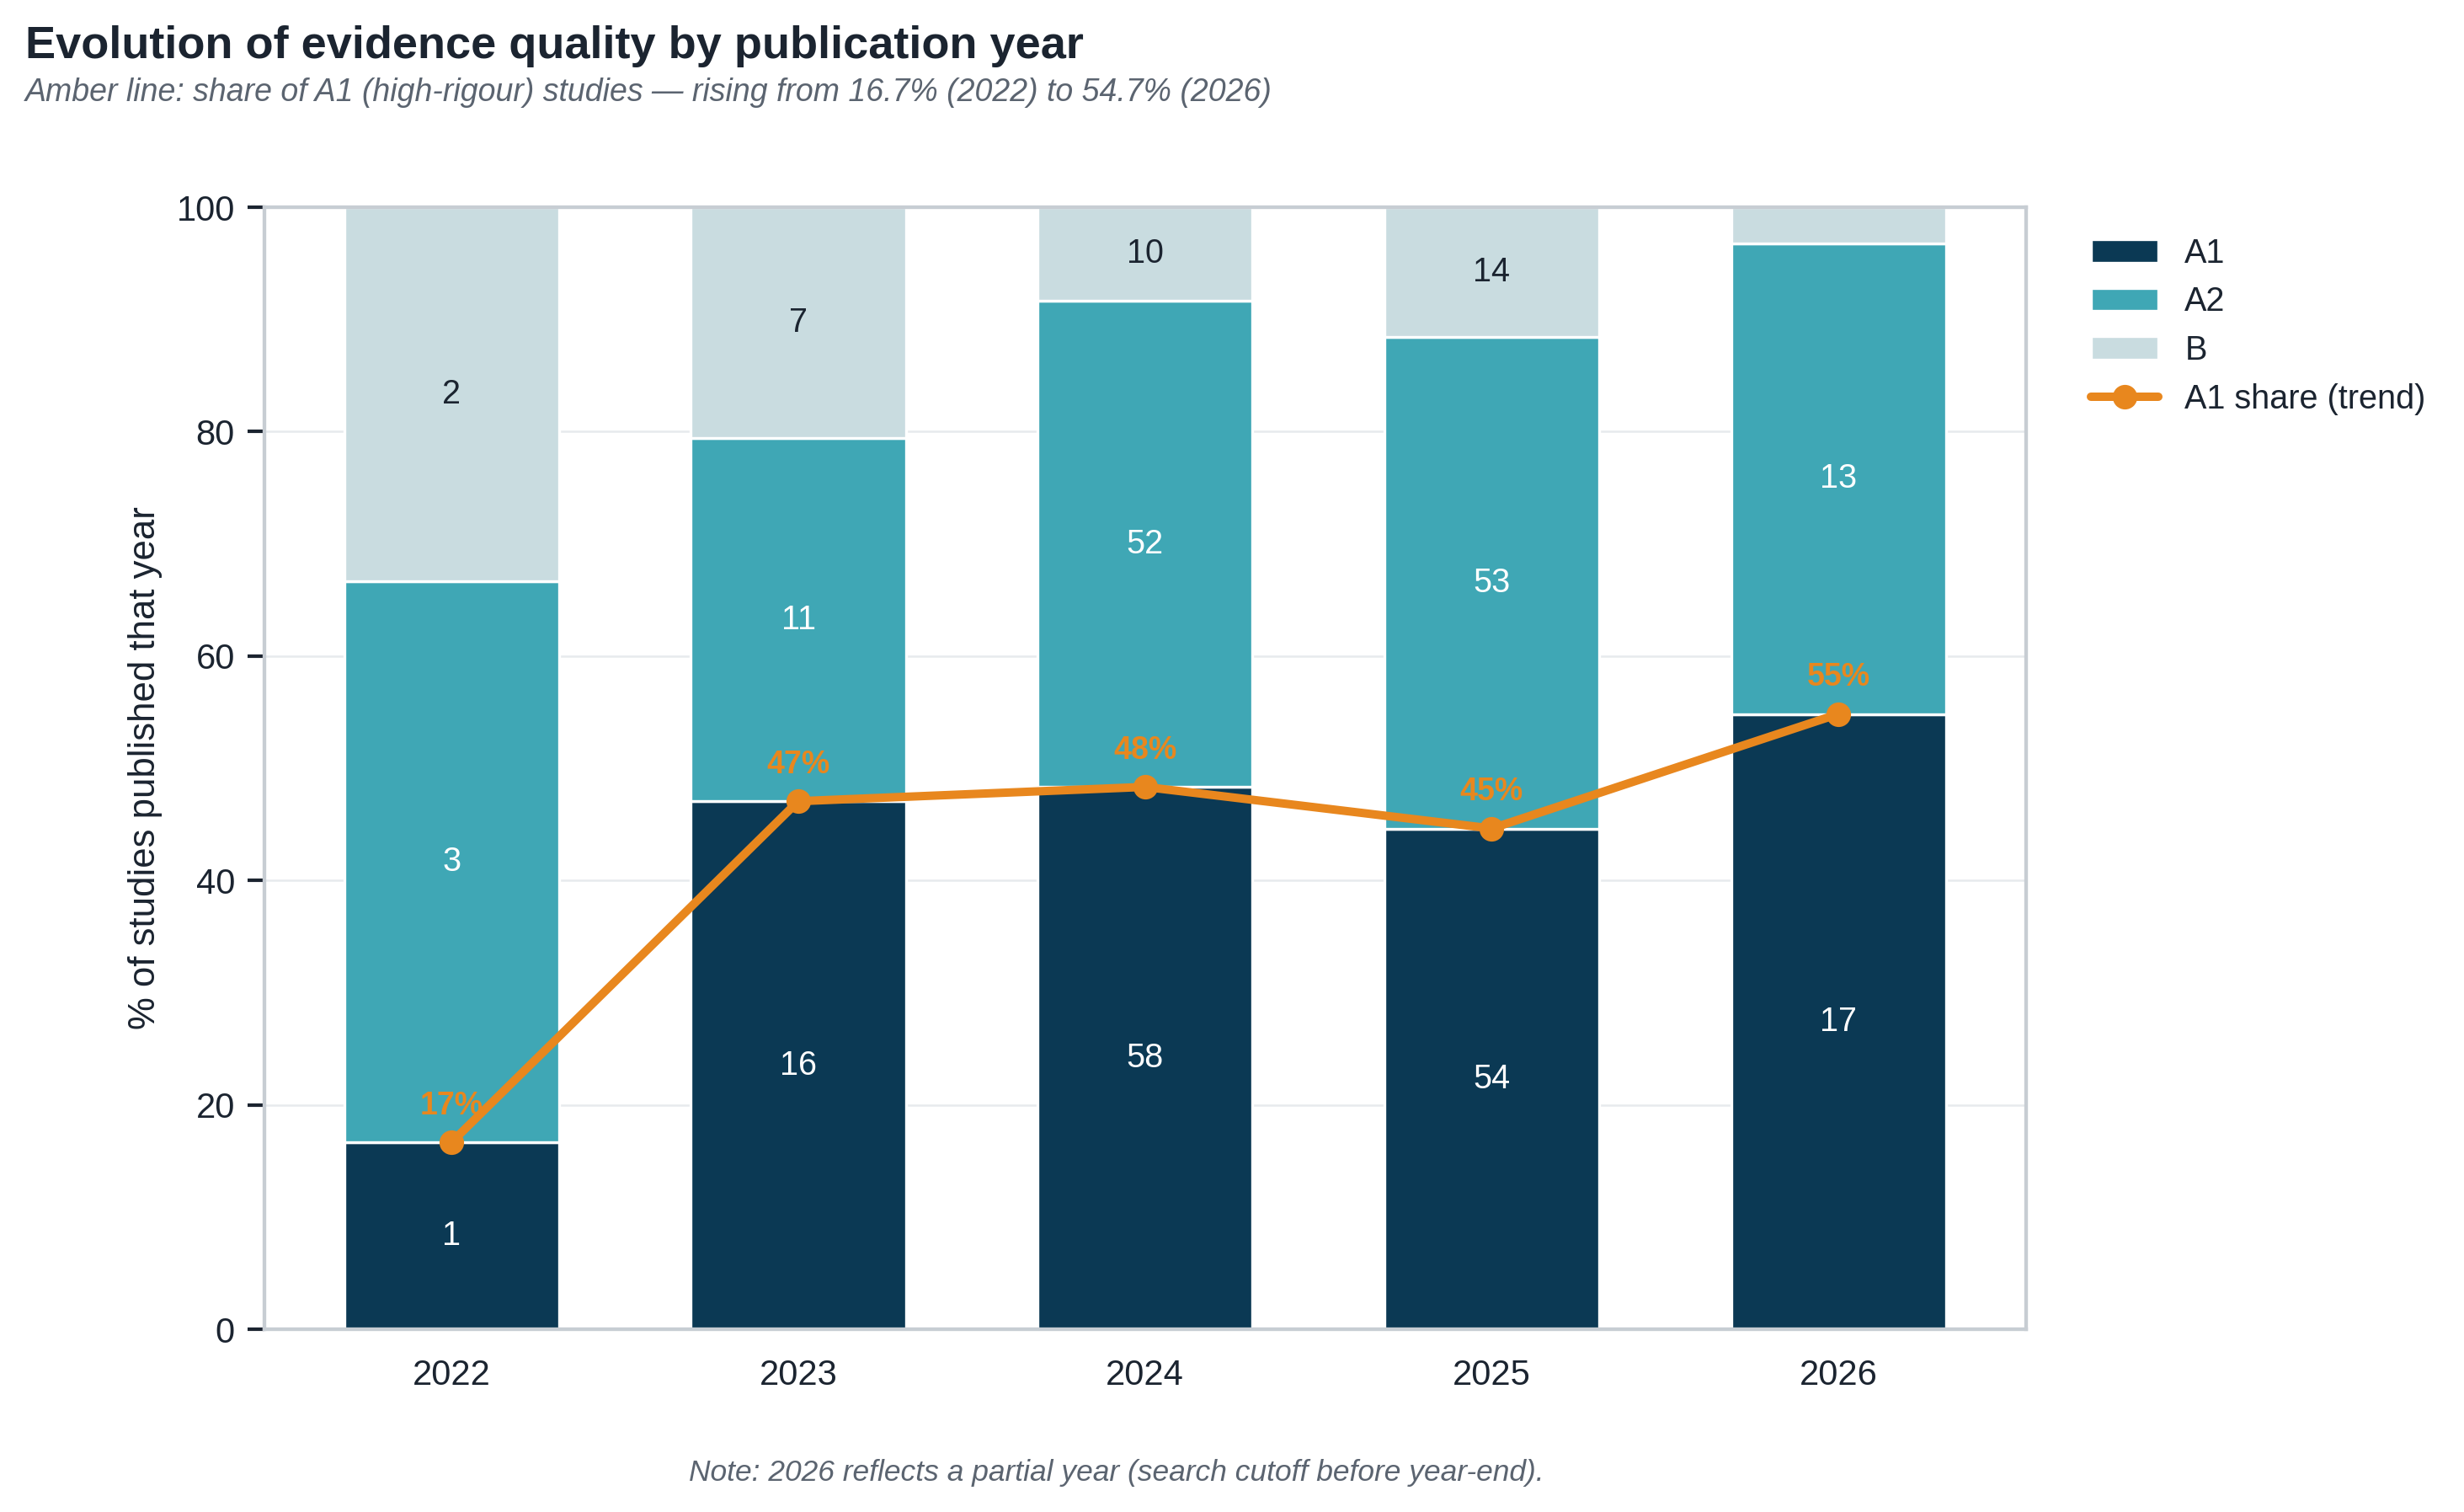
\includegraphics[width=0.82\linewidth]{figures/B3_quality_evolution_by_year.png}
    \caption{Evolution of evidence quality by publication year. The amber line tracks the share of A1 (high-rigour) studies.}
    \label{fig:quality_evolution}
\end{figure}

This classification enables a weighted synthesis, where conclusions are primarily grounded in stronger empirical evidence and in CORE studies, with SUPPORTING and PERIPHERAL evidence used for triangulation and contextualisation. It also reveals a clear concentration of research efforts on the technical reliability of AI-generated code and on the dynamics of human--AI interaction, with comparatively limited attention to organisational, economic, and cognitive dimensions.
% 3.1 ends here

% 3.2 starts here
\subsection{Code Quality and Technical Debt}
\label{sec:cqtd}
Code quality and technical debt is the largest and most extensively developed dimension in the corpus, accounting for 45.2\% of studies (n=141; Section~\ref{sec:corpus-profile}). Evidence in this dimension converges on a structural pattern: AI-assisted programming reliably produces code that satisfies narrow, benchmark-style correctness criteria, but this performance does not transfer cleanly to the conditions under which software is actually maintained, secured, and integrated. The following sub-sections trace this pattern across benchmark performance, real-world generalisation, defect and structural error rates, security vulnerabilities, maintainability and dependency management, multi-turn and agentic effects, and human-versus-AI comparisons.

\subsubsection{Benchmark Performance and the Realism Gap}
\label{sec:cqtd-benchmark}
Synthetic benchmarks remain the most common instrument for evaluating AI-generated code, and the corpus confirms that strong benchmark performance is achievable: Claude Sonnet 4 reached a 95.1\% success rate on the 164-problem HumanEval Python benchmark, with comparable assistant evaluations reporting success rates around 40\% under more varied task-difficulty conditions. However, this performance does not reliably predict repository-level code quality or maintenance outcomes, a pattern supported by seven studies spanning benchmark evaluation, repository mining, patch analysis, and agentic evaluation \cite{idrisov_program_2024,bayram_comparative_2025,chen_evaluating_2024,aleithan_swe-bench_2024,abbassi_recatcher_2025,zheng_top_2025,dou_whats_2026}. When stricter, EvalPlus-style hidden-test regimes are applied to the same benchmarks, apparent pass@k performance drops by as much as 28.9\%, indicating that headline benchmark figures substantially overstate functional reliability under more rigorous testing \cite{liu_is_2023}.

This realism gap widens further at repository scale. Agentic systems evaluated on real-world GitHub issues, such as SWE-Bench-style benchmarks, report repair rates around 31--33\%, and stricter data-quality filtering on the same benchmark family can lower resolution rates to below 4\% \cite{aleithan_swe-bench_2024,chen_evaluating_2024}. A large-scale repository-mining study of 304,362 verified AI-authored commits similarly finds that benchmark-level success coexists with persistent technical debt once code is merged into production codebases \cite{liu_debt_2026}. Taken together, these results indicate that benchmark pass rates and repository-level reliability are only weakly coupled, and that claims of AI coding competence drawn solely from synthetic benchmarks should be treated as bounded rather than generalisable.

\subsubsection{Defect Rates and Structural Error Patterns}
\label{sec:cqtd-defects}
Beyond benchmark-specific failure, the corpus documents substantial and recurring defect rates in AI-generated code under realistic evaluation conditions. One large-scale quality analysis of ChatGPT-generated Python code found that 76.46\% of generated snippets and 84.51\% of modified snippets contained at least one quality issue \cite{rabbi_ai_2024}. Studies focused specifically on bug characterisation report that a meaningful share of generated solutions fail to produce functional code even after revision, with one defect-characterisation study finding 19.51\% of cases unable to generate a working solution \cite{esfahani_understanding_2024}, and a code-translation study attributing 33.5\% of translation bugs to data-handling errors rather than syntactic mistakes \cite{pan_lost_2024}. Regression-testing evidence adds a further layer: fine-tuning or adapting models across programming languages can introduce syntax regressions of up to 12\%, even when the underlying generation capability appears to improve \cite{abbassi_recatcher_2025}.

These structural error patterns are corroborated by the broader consensus evidence in the corpus, which identifies persistent technical debt after merging as a strong, repeatedly observed pattern across repository mining, pull-request analysis, and patch-safety studies \cite{liu_debt_2026,borg_echoes_2026,siddiq_quality_2024,cotroneo_devaic_2025,sajadi_how_2025,fu_security_2025,schreiber_security_2026}. Critically, code that passes immediate functional checks can still carry latent maintenance or security liabilities that surface only once it is exercised under real usage conditions, indicating that defect rates measured at generation time systematically understate downstream risk.

\subsubsection{Security Vulnerability Exposure}
\label{sec:cqtd-security}
Security vulnerability is the most thoroughly evidenced sub-theme in the corpus, with ten studies converging on a strong consensus claim: security vulnerabilities are systematically introduced into AI-generated code, but the precise risk profile depends on programming language, CWE family, task type, and prompting context \cite{pearce_asleep_2025,siddiq_generate_2023,schreiber_security_2026,asare_is_2024,alrashedy_can_2024,fu_security_2025,dozono_large_2026,tony_prompting_2025,res_enhancing_2024,asare_user-centered_2024}. Reported vulnerability rates vary considerably with evaluation design: foundational work on GitHub Copilot found that approximately 40\% of generated programs in security-relevant scenarios were vulnerable \cite{pearce_asleep_2025}, while large-sample evaluations such as SALLMS assessed security properties across 17,000 generated samples \cite{siddiq_generate_2023}, and comparative human-versus-AI studies report vulnerability rates around 33--49\% depending on the comparison baseline \cite{asare_is_2024}.

Security repair is consistently weaker and less reliable than security diagnosis, a moderate-consensus pattern supported across eight studies \cite{alrashedy_can_2024,dozono_large_2026,belozerov_secure_2026,sajadi_how_2025,tony_prompting_2025,res_enhancing_2024,pearce_asleep_2025,fu_security_2025}. Repair-oriented evaluations report partial success at best, with patch-level repair outcomes in the range of 16--27\% depending on vulnerability type and repair strategy \cite{alrashedy_can_2024}. At the same time, prompt-engineering interventions show that mitigation is genuinely possible: targeted prompt design reduced insecure generated samples by up to 16\% \cite{res_enhancing_2024}, while structured prompting techniques raised the proportion of secure code by as much as 85\% in one study \cite{tony_prompting_2025}. This indicates that security risk in AI-generated code is conditional and addressable through deliberate intervention, rather than an immutable property of the underlying models, but that such mitigation requires active human effort rather than occurring by default.

\subsubsection{Maintainability, Complexity, and Dependency Management}
\label{sec:cqtd-maintainability}
Maintainability evidence in the corpus is mixed in a specific and informative way: AI-generated code can be concise or superficially readable in narrow tasks while simultaneously accumulating code smells, duplication, structural complexity, or downstream maintenance burden, a strong-consensus pattern supported by six studies using metric-based, pull-request-based, and downstream-tracking designs \cite{idrisov_program_2024,rabbi_ai_2024,borg_echoes_2026,chen_evaluating_2024,dou_whats_2026,gao_treat_2025}. In some constrained tasks, AI-generated solutions used markedly fewer lines of code than human-written equivalents, with reductions of up to 60--86\% in selected benchmark tasks \cite{idrisov_program_2024}; however, this brevity does not consistently correspond to lower long-term maintenance cost. A large-scale empirical study of AI-generated code in production repositories found that 89.1\% of identified issues were classified as code smells, with 24.2\% of affected code surviving long-term and 41.1\% of security-relevant flaws persisting in the codebase after merge \cite{liu_debt_2026}.

Dependency, import, and reproducibility failures emerge as a distinct and systematic sub-theme rather than a minor extension of functional correctness, supported by a moderate consensus across eight studies \cite{vangala_ai-generated_2026,twist_library_2025,latendresse_how_2025,zheng_top_2025,chen_evaluating_2024,tian_codehalu_2025,liu_debt_2026}. An empirical study of dependency gaps in LLM-based coding agents reported dependency-related failure figures as high as 89.2\%, alongside a 44.0\% rate of incomplete or misspecified listed dependencies \cite{vangala_ai-generated_2026}. Library hallucination, where generated code references packages or APIs that do not exist or do not match the specified version, is documented as a recurring and separately diagnosable failure mode \cite{twist_library_2025,latendresse_how_2025}, reinforcing the case that reproducibility and dependency management constitute a CQTD concern in their own right rather than a symptom of generic incorrectness.

\subsubsection{Multi-Turn Interaction and Agentic Effects}
\label{sec:cqtd-multiturn}
A further moderate-consensus pattern, supported by eight studies, establishes that multi-turn interaction and agentic workflows do not monotonically improve code quality: depending on trajectory, additional turns or additional tool autonomy can repair, preserve, or amplify defects \cite{chen_evaluating_2024,vangala_ai-generated_2026,kozak_when_2025,zhong_developer-llm_2025,sajadi_how_2025,abbassi_recatcher_2025,honarvar_turbulence_2025,aleithan_swe-bench_2024}. An analysis of developer-LLM conversations found that import-related errors decreased from 48.3\% to 44.6\% across successive conversational turns, indicating genuine but incomplete improvement through iteration \cite{zhong_developer-llm_2025}. Agentic patch evaluation across 4,892 patches from ten different coding agents revealed divergent file- and function-level modification patterns relative to gold-standard patches, showing that increased autonomy expands the surface area over which quality and security risk can manifest \cite{chen_evaluating_2024}. This expansion of risk surface with autonomy is itself a moderate-consensus finding, supported by evidence that insecure agentic behaviours occur at rates including 21\% and 56.61\% depending on the study and task setting \cite{kozak_when_2025}. A benchmark that reconstructs the exact repository state and natural-language requirement under which a human developer originally introduced a real-world vulnerability extends this picture with more fine-grained, agent-specific evidence: across three popular code agents and five backbone LLMs, the best-performing combination produced output that was both functionally correct and free of the reconstructed vulnerability in only 23.8\% of cases, and an agent's likelihood of introducing a given vulnerability type was largely unrelated to how frequently that type occurred in the underlying dataset \cite{chen_securevibebench_2026}. The same benchmark further shows that command-line agentic interfaces, despite achieving the highest functional correctness among all evaluated configurations, did not achieve correspondingly high security rates, indicating that scaffolds optimised for completing a task can systematically under-prioritise the security of the result.

These dynamics connect directly to verification and modification effort, which the corpus shows only partially offsets generation-speed gains rather than eliminating the need for human oversight \cite{idrisov_program_2024,tang_developer_2024,zhong_developer-llm_2025,siddiq_quality_2024,bose_prompts_2025,abbassi_recatcher_2025,tian_codehalu_2025}. In one controlled comparison, incorrect but minimally modifiable code occurred in 8.7\% of generated outputs, with time savings from correcting near-correct code ranging from 8.9\% to 71.3\% relative to writing code from scratch \cite{idrisov_program_2024}. Eye-tracking and IDE-action studies of developer validation behaviour confirm that this verification work is cognitively substantive rather than perfunctory, requiring developers to actively trace logic and confirm correctness rather than passively accepting AI-generated suggestions \cite{tang_developer_2024}.

\subsubsection{Human-versus-AI Quality Comparisons}
\label{sec:cqtd-human-vs-ai}
Direct comparisons between human-written and AI-generated code are consistently context-dependent rather than categorical, a strong-consensus pattern supported by eight studies: AI systems can outperform human baselines on some surface metrics while underperforming on correctness, security, or maintainability in other settings \cite{idrisov_program_2024,bayram_comparative_2025,cotroneo_devaic_2025,asare_is_2024,rabbi_ai_2024,siddiq_quality_2024,borg_echoes_2026,pearce_asleep_2025}. In one comparative study, GitHub Copilot solved 50.0\% of a curated task set while the broader evaluated AI tool set solved only 20.6\% of tasks overall, illustrating substantial variation even among AI systems evaluated under the same conditions \cite{idrisov_program_2024}. At the same time, the strongest current models achieve benchmark scores that meet or exceed typical human baselines on narrow, well-specified tasks, with top-performing models reaching 95.1\% and 94.5\% on HumanEval in one comparative analysis \cite{bayram_comparative_2025}.

The direction of this comparison reverses, however, once security and downstream maintainability are taken into account: studies comparing Copilot's behaviour regarding vulnerability introduction with that of human developers, and studies tracking downstream maintainability effects, both indicate that AI-generated code does not categorically outperform human-written code once these dimensions are considered \cite{asare_is_2024,borg_echoes_2026}. This reversal is the empirical basis for treating correctness, security, maintainability, reproducibility, and human validation as analytically separate constructs within CQTD rather than collapsing them into a single quality score, a strong-consensus conclusion supported by seven studies spanning repository-scale, downstream, reproducibility, validation, and regression-testing designs \cite{liu_debt_2026,schreiber_security_2026,borg_echoes_2026,vangala_ai-generated_2026,tang_developer_2024,siddiq_quality_2024,abbassi_recatcher_2025}.

\subsubsection{Synthesis}
\label{sec:cqtd-synthesis}
Across all seven sub-themes, the CQTD evidence base converges on a single structural conclusion: generation efficiency in AI-assisted programming is empirically real, but it is systematically and substantially offset by verification overhead. Strong benchmark performance, concise output, and partial security mitigation are all genuine and well-documented capabilities; equally well documented are the realism gap between benchmark and repository-level performance, the persistence of technical debt and security vulnerabilities after merge, the non-monotonic effect of additional interaction turns and agentic autonomy, and the necessity of treating correctness, security, maintainability, and reproducibility as distinct rather than interchangeable quality constructs. This pattern provides the most methodologically robust empirical grounding in the corpus for the verification-overhead component of the socio-technical equilibrium framework developed in this study, a connection examined further in the Discussion.
%3.2 ends here

%3.3 starts here
\subsection{Human--AI Interaction}
\label{sec:hai}
Human--AI interaction is the second-largest dimension in the corpus, accounting for 36.9\% of studies (n=115; Section~\ref{sec:corpus-profile}). The evidence base for this dimension is organised around seven sub-themes: prompting dynamics and conversational strategies, workflow integration and collaboration patterns, trust and reliance behaviour, developer experience and perceived value, learning and educational contexts, robustness and agentic reliability, and identity and socio-professional continuity. Across these sub-themes, AI-assisted programming appears less as a replacement of developer expertise than as a reconfiguration of interaction, verification, judgement, and responsibility: developers do not simply receive code, they negotiate it.

\subsubsection{Prompting Dynamics and Conversational Strategies}
\label{sec:hai-prompting}
Prompting functions as the interaction infrastructure of AI-assisted programming rather than as a generic natural-language skill. Developers express intent, surface local context, specify constraints, and negotiate the form of repair, explanation, or continuation needed to make a generated artefact usable \cite{nam_understanding_2025,barke_grounded_2023,khojah_beyond_2024}. This positions prompting as situated software work: professional use involves assembling task goals, surrounding code, desired edit behaviour, and follow-up constraints into an interaction that progressively shapes model output. This interaction channel is technically consequential rather than cosmetic. Ambiguous, contradictory, and incomplete task descriptions degrade code-model robustness \cite{larbi_when_2025}; semantically preserving natural-language perturbations can still alter results \cite{chen_nlperturbator_2026}; and faulty premises can mislead generation unless critical checking is incorporated into the interaction \cite{li_refining_2025}. Quantitative robustness evidence reinforces this point directly: only 27.43\% of GitHub Copilot paraphrase cases preserved the same correct output across semantically equivalent prompt variants \cite{mastropaolo_robustness_2023}, and both superficial programming-problem transformations and simulated Copilot-style completion context measurably alter reliability \cite{shirafuji_exploring_2023,jiang_simcopilot_2025}. Prompting can also span the full development lifecycle rather than isolated code requests, proceeding through cycles of generation, inspection, correction, and continuation from requirements through documentation \cite{li_prompting_2024,fayed_prompt-driven_2026,waseem_chatgpt_2024}.

\subsubsection{Workflow Integration and Collaboration Patterns}
\label{sec:hai-workflow}
AI assistance shifts developer work rather than removing it. The central workflow change is a redistribution of labour towards reading, editing, rejection, validation, orchestration, and trace management \cite{mozannar_reading_2024,stray_generative_2025,xia_agentless_2024}. One influential cost model frames AI-assisted programming explicitly in these terms: the value of a generated suggestion depends on the time and effort required to read, understand, and repair it, not on how quickly text appears \cite{mozannar_reading_2024}. This redistribution is visible both in everyday solo and pair programming, where Copilot and ChatGPT change how developers move between assistance, oversight, interruption, and collaborative sense-making \cite{stray_generative_2025}, and in automated program repair, where localisation, patch generation, and validation must be explicitly orchestrated for the repair process to function at all \cite{xia_agentless_2024}. Collaborative-trace evidence extends this workflow claim beyond the editor: shared ChatGPT conversations appeared in 33.2\% of pull-request conversations and 36.9\% of issue conversations in one large-scale GitHub corpus \cite{hao_empirical_2024}, with related evidence on AI-generated code and self-admitted generative-AI use confirming that this delegation-with-validation pattern is already embedded in open-source project artefacts \cite{grewal_analyzing_2024,tufano_developers_2026}. In-IDE generation studies corroborate the same pattern at the individual level: developers remain responsible for inspecting and adapting generated code rather than accepting it outright \cite{xu_-ide_2022}, and increasing automation moves work towards specification, monitoring, verification, and repair rather than eliminating it \cite{chen_code_2025}.

\subsubsection{Trust, Verification, and Reliance Behaviour}
\label{sec:hai-trust}
Effective human--AI interaction depends on calibrated reliance rather than generic trust. Acceptance of AI-generated suggestions is shaped by perceived quality, contextual fit, controllability, effort awareness, and developers' capacity to verify outputs \cite{brown_identifying_2024,wang_investigating_2024,dibia_aligning_2023}. Trust-calibration mechanisms, including explicit indicators and controllability features, are something developers actively want rather than already have by default \cite{wang_investigating_2024}, and human judgements of code-generation value correlate with perceived accuracy and required effort in ways that offline metrics alone cannot explain \cite{dibia_aligning_2023}. Security-sensitive reliance introduces a sharper boundary condition for this calibration: developers using AI assistants can write more insecure code while simultaneously reporting higher confidence in that code \cite{perry_users_2023}, a pattern corroborated by qualitative evidence on security practices and concerns among AI-assisted developers \cite{klemmer_using_2024} and by memorisation risks that complicate claims about LLM-based program repair \cite{kong_demystifying_2025}. Trust is therefore best understood as an interaction outcome, produced through inspectability, validation, domain-aware checks, and the explicit option to accept, reject, repair, or test, rather than as a static property of either the tool or the developer.

\subsubsection{Developer Experience, Usability, and Perceived Value}
\label{sec:hai-experience}
Positive experience and continuance are important adoption signals, but the evidence is consistent that they do not establish engineering benefit on their own. Satisfaction, code volume, and perceived acceleration can coexist with inspection, debugging, confidentiality, accessibility, and integration costs \cite{santos_model-assisted_2025,park_continuance_2025,mozannar_reading_2024}. Professional practitioners value LLM support while explicitly retaining responsibility for judgement and integration \cite{santos_model-assisted_2025}, and survey evidence from industry developers shows that continuance reflects perceived usefulness and fit rather than independently measured correctness or maintainability \cite{park_continuance_2025}. Usability concerns in this sub-theme are socio-technical rather than purely interface-level: accessibility-specific benefits and frictions have been documented for visually impaired developers using coding assistants \cite{flores-saviaga_impact_2025}, and AI Skill Threat was reported to affect 43--45\% of surveyed developers, linking tool adoption directly to professional identity and thriving \cite{hicks_new_2024}. Taken together, this sub-theme indicates that perceived value is real but bounded: experience evidence improves understanding of adoption, but it cannot substitute for validation-based quality evidence.

\subsubsection{Learning, Novices, and Educational Contexts}
\label{sec:hai-learning}
Educational evidence shows a persistent comprehension-performance gap: AI assistance can raise visible task progress for novices while leaving comprehension, testing ability, and durable transfer uncertain \cite{prather_its_2024,qiao_comprehension-performance_2025,shah_students_2025}. Novice programmers experience tools such as Copilot as usable and sometimes surprisingly anticipatory, but this fluency can obscure what learners actually understand \cite{prather_its_2024}, a divergence explicitly framed as a comprehension-performance gap in GenAI-assisted brownfield programming \cite{qiao_comprehension-performance_2025}. Working with unfamiliar, large code bases further increases the need for review, testing, and sense-making among student users \cite{shah_students_2025}. Quantitative evidence on over-reliance is direct: 90\% of students in one study expressed over-reliance concerns even while recognising the benefits of AI code completion \cite{takerngsaksiri_students_2024}. This pattern is reinforced by evidence that prompt engineering itself must be learned as an interaction practice in introductory programming contexts \cite{denny_conversing_2023}, and that semester-long classroom collaboration with generative AI changes peer-like interaction dynamics in ways that require deliberate instructional scaffolding \cite{lyu_will_2025}. Educational use of AI-assisted programming should therefore actively force explanation, testing, reflection, and recovery strategies, so that visible task completion does not mask fragile understanding.

\subsubsection{Robustness, Prompt Sensitivity, and Agentic Reliability}
\label{sec:hai-robustness}
Developer-facing reliability is a system property: it depends on prompt quality, semantic stability, retrieval, localisation, patch generation, validation, runtime behaviour, and benchmark validity, rather than on single-run functional success alone \cite{xia_agentless_2024,olausson_is_2024,agarwal_copilot_2024,liu_e2edev_2026}. Agentless decomposes LLM-based repair into localisation, patch generation, and validation stages, making each stage a potential reliability bottleneck in its own right \cite{xia_agentless_2024}, and self-repair is explicitly shown not to be a universal solution to code-generation failures \cite{olausson_is_2024}. Evaluation-harness evidence reinforces that LLM-guided programming requires dedicated infrastructure for assessing reliability rather than relying on benchmark pass rates alone \cite{agarwal_copilot_2024}, and end-to-end development benchmarking exposes multi-step coordination demands that isolated code-generation tasks do not capture \cite{liu_e2edev_2026}. A comprehensive comparison of seven general-purpose agent frameworks across software development, vulnerability detection, and program repair tasks shows that this coordination demand is not merely a cost to be managed but can actively undermine effectiveness: single-agent frameworks outperformed multi-agent frameworks on most tasks, with the multi-agent systems' longer reasoning trajectories and higher correction rates reflecting information loss and inter-agent error propagation rather than more thorough problem-solving \cite{yin_comprehensive_2025}. Robustness claims become especially fragile under further scrutiny: self-consistency evaluation reveals that models can fail to reproduce their own correct outputs across semantically equivalent reformulations \cite{min_beyond_2024}, and models can be shown to exploit test cases directly rather than solving the underlying task \cite{zhong_impossiblebench_2025}. Robustness in human--AI interaction is therefore produced by the interaction between user specification, repository context, orchestration design, validation tooling, runtime constraints, and benchmark assumptions, not by any single one of these factors in isolation.

\subsubsection{Identity, Accessibility, and Socio-Professional Continuity}
\label{sec:hai-identity}
Human--AI interaction also affects professional continuity by shaping identity, perceived skill threat, accessibility, inclusion, and cross-role communication. This sub-theme is less evenly evidenced than prompting, workflow, trust, or robustness, but the available evidence is informative. AI Skill Threat was found to affect 43--45\% of surveyed developers, tying tool adoption directly to professional identity, thriving, and the meaning of developer expertise \cite{hicks_new_2024}. Generative AI coding assistants have also been shown to change the work of visually impaired developers by altering code navigation, explanation, and interaction, introducing frictions that studies of sighted users alone would not surface \cite{flores-saviaga_impact_2025}. Organisational adoption research adds that uptake depends on task fit, confidentiality, and local context rather than on tool capability alone \cite{davila_industry_2024}, and mixed-methods evidence shows that human--AI collaboration changes how developers coordinate assistance and oversight at the team level \cite{stray_human-ai_2025}. Cross-role evidence on reverse engineering and agile-epic evaluation extends this concern to artefact review and cross-role communication, though this evidence should be read as a cautious scope extension rather than as direct corroboration of identity-level change \cite{surk_reducing_2026}. Human--AI interaction is therefore not only a coding interface; it can reshape who participates in software development, how expertise is recognised, and how responsibility is negotiated.

\subsubsection{Synthesis}
\label{sec:hai-synthesis}
Across all seven sub-themes, the HAI evidence base converges on a structural account in which interaction quality and trust calibration jointly determine whether generation efficiency is converted into dependable engineering value or displaced into hidden risk. Prompting, contextualisation, conversational repair, and representation choices shape the reliability and usefulness of AI-generated outputs across professional, educational, and agentic settings; trust calibration regulates whether developers accept, revise, test, or reject plausible but potentially incorrect or insecure suggestions. Cognitive redistribution connects these mechanisms by shifting developer effort away from direct code construction and towards supervision, orchestration, explanation, and decision-making. This pattern provides the empirical grounding in the corpus for treating interaction quality and trust calibration as the primary HAI constructs within the socio-technical equilibrium framework, and for understanding verification overhead, documented extensively in the CQTD dimension (Section~\ref{sec:cqtd}), as something that is actively managed or amplified through the quality of human--AI interaction rather than fixed in advance. This connection is examined further in the Discussion.
%3.3 ends here

%3.4 starts heres
\subsection{Productivity}
\label{sec:productivity}
Productivity is the third-largest dimension in the corpus, accounting for 8.3\% of studies (n=26; Section~\ref{sec:corpus-profile}). AI assistance improves productivity most reliably when programming work is local, well specified, and readily verifiable, but the corpus does not support a universal acceleration claim. Controlled and benchmark-like studies show substantial generation efficiency: ChatGPT outperformed Stack Overflow on algorithmic and library-use tasks, including reported algorithmic task-score contrasts of 72.0 versus 0.0 and an average of 38.7 versus 5.0 in the relevant comparison \cite{liu_chatgpt_2023}. Complexity then narrows the effect. ChatGPT-3.5 solved 92\% of easy, 79\% of medium, and 51\% of hard coding problems in one complexity-stratified evaluation, with prompt engineering improving results but not removing the complexity gradient \cite{li_evaluating_2024}. A separate difficulty-level study reported complex-problem performance at just 4.3\%, indicating that decomposition and iteration are part of the work rather than optional refinements \cite{yan_closer_2023}.

Brownfield and field evidence makes the productivity claim more conditional. In computing-student brownfield tasks, Copilot reduced completion time by 34.9\%, increased solution progress by 50\%, and reduced manual typing and web search by 10.6\% and 11.6\% respectively \cite{shihab_effects_2025}. This supports a positive productivity mechanism: assistants can lower the cost of producing plausible edits, scaffolding searches and repetitive implementation steps. However, experienced open-source maintainers in a field experiment took 19\% longer with AI assistance, despite predicting a 24\% speed-up before the task and estimating afterwards that the tool had made them 20\% faster \cite{becker_measuring_2025}. This contradiction is not noise; it marks the difference between local generation and situated software engineering, where repository context, testing, review, and integration can dominate raw output speed.

Enterprise evidence reinforces this interpretation. Developers using an enterprise AI code assistant modified outputs and treated checking as a normal part of use, so generated code functioned as a draft requiring human validation rather than as a finished artefact \cite{weisz_examining_2025}. Across these studies, the relevant productivity unit is therefore not the suggestion, the line of code, or even the completed task in isolation: it is the net work required to move from generated candidate to accepted, maintainable project change. Productivity gains are strongest where the generated artefact is easy to inspect and weak where the artefact requires deep contextual reasoning, cross-file consistency, security judgement, or domain-specific integration.

A persistent limitation across this sub-literature is that productivity studies rarely measure speed, correctness, rework, and downstream integration within the same design. Some quantify completion time or task scores, while others observe acceptance, behaviour, or perceptions, making the evidence strong for conditional acceleration but weaker for total development productivity across real projects. The most defensible synthesis is that AI assistance increases generation efficiency, while its contribution to net productivity depends on whether verification overhead remains smaller than the construction effort saved. This positions productivity as the dimension in the corpus where the trade-off between generation efficiency and verification overhead, central to the socio-technical equilibrium framework, is most directly observable, a connection examined further in the Discussion.
%3.4 ends here

%3.5 starts here
\subsection{Perception and Trust}
\label{sec:perception-trust}
Perception and Trust is the fourth-largest dimension in the corpus, accounting for 4.2\% of studies (n=13; Section~\ref{sec:corpus-profile}). The evidence shows that developers often regard AI coding assistants as useful, but trust is selective, contextual, and vulnerable to miscalibration. In a broad developer survey, 84\% of 481 respondents reported using AI-based coding assistants, indicating that adoption is already normalised rather than experimental \cite{sergeyuk_using_2025}. A separate survey of 207 developers found that 73\% perceived productivity improvement from ChatGPT in software development \cite{vaillant_developers_2024}. These results establish perceived usefulness, but they do not by themselves establish dependable software outcomes; perception evidence becomes meaningful only when read against task difficulty, correctness evidence, and security risk.

Task difficulty is the clearest calibration boundary. Kuhail and colleagues reported 73\% success on easy problems versus 10\% on hard problems across 180 problems and 99 developers, which explains why favourable perceptions are more defensible for routine work than for complex development \cite{kuhail_will_2024}. Acceptance conditions also matter: Suryavanshi and colleagues found that behavioural intention was associated with use behaviour, with a reported coefficient of $\beta=0.419$, linking acceptance to facilitating conditions, perceived usefulness, perceived ease of use, and hedonic motivation \cite{suryavanshi_integrating_2025}. Trust is therefore not a static attitude towards a tool; it is shaped by the local conditions that make use feasible, rewarding, and apparently safe.

The strongest caution comes from security and hallucination evidence. Developers report that generative AI can make their code less secure, shifting trust from the generated artefact to inspection and security review \cite{kudriavtseva_my_2025}. Empirical secure-code assessment also shows uneven LLM performance across languages, so trust cannot be detached from the target language and vulnerability type \cite{dozono_large_2026}. Code hallucination evidence further shows that fluent code-like output can contain execution-relevant failures, making over-reliance dangerous when developers treat plausibility as correctness \cite{tian_codehalu_2025}. Trust calibration therefore requires repeated evidence about when the assistant is likely to be correct, not only a general belief that the assistant is helpful.

Interpretability-oriented evidence offers a constructive response to this miscalibration risk. A syntax-grounded explanation method that maps model confidence onto abstract-syntax-tree categories was found to support more accurate trust judgements than either a flat sequential display of token probabilities or no explanation at all: participants given the AST-based explanation were more likely to judge the underlying model as unreliable, and none judged it as highly reliable, compared with participants given only sequential probabilities, of whom 29\% judged the model highly reliable despite the same underlying errors in every scenario \cite{palacio_towards_2025}. This result reframes trust calibration as something that can be actively supported by interpretability tooling rather than left to a developer's unaided judgement: explanations that expose where a model's confidence is weak help pre-empt the kind of unwarranted confidence that the security and hallucination evidence above warns against.

Qualitative trust evidence makes this dynamic explicit. Developers define, grant, revise, and withdraw trust as they observe tool behaviour, task fit, and failure modes \cite{sabouri_trust_2025}. The key empirical pattern is thus a perception-reality gap: developers can experience acceleration and convenience while still needing to detect hallucinated dependencies, insecure code, weak reasoning, or contextually inappropriate suggestions. A persistent limitation is that many perception studies rely on self-report and are not consistently paired with objective code quality, security, or maintenance outcomes. Nevertheless, the combined evidence supports a strong synthesis: trustworthy AI-assisted programming is not produced by higher confidence or more frequent use, but by calibrated reliance under explicit evidence of correctness, task difficulty, and risk. This positions Perception and Trust as the dimension in the corpus most directly anchoring the trust-calibration construct of the socio-technical equilibrium framework, a connection examined further in the Discussion.
%3.5 ends here

%3.6 starts here
\subsection{Cognitive Load and Human Factors}
\label{sec:cognitive-load}
Cognitive Load and Human Factors is the fifth-largest dimension in the corpus, accounting for 2.9\% of studies (n=9; Section~\ref{sec:corpus-profile}). AI assistance changes the distribution of cognitive work rather than simply reducing it. The strongest behavioural evidence shows that developers spend substantial attention on interacting with and checking AI outputs: Mozannar and colleagues report that 51.5\% of interaction time was spent in AI-related activities, with verification alone accounting for 22.4\%, and suggestion acceptance around 34\% \cite{mozannar_reading_2024}. This finding reframes the assistant as a generator of supervisory work: developers may write less code manually, but they must read, judge, compare, test, and decide whether the generated output is appropriate for the task.

A controlled experiment with 109 participants substantiates this redistribution directly by tracing how developers exercised, or failed to exercise, that supervisory work. Working with ChatGPT improved efficiency on simple, well-specified coding puzzles but not on a typical small-scale development task requiring developers to fix bugs in an existing codebase, and it did not improve solution quality in either setting \cite{wang_rocks_2024}. Screen-history analysis of how participants interacted with the assistant explains this gap: roughly one third of participants on the development task tried to delegate the entire problem to ChatGPT without first attempting to understand the code themselves, and this group most often gave up or produced very low-quality solutions; by contrast, close to half of participants treated the assistant as a collaborator, alternating between asking it to explain unfamiliar code, proposing a fix, and pointing out concrete errors in its output before accepting a revision. This contrast indicates that cognitive redistribution is conditional on developers retaining and exercising comprehension, not an automatic consequence of using an AI assistant.

Educational and brownfield evidence supports the same redistribution pattern. In a self-paced CS1 setting, 33 novices produced 1,666 Codex interactions, showing extensive use of generation and explanation to progress through programming tasks \cite{kazemitabaar_how_2023}. This indicates construction support, but also a need for output interpretation and judgement. In brownfield programming, Qiao and colleagues report a comprehension-performance gap: GenAI assistance can support task completion more than program understanding when developers work with existing code \cite{qiao_comprehension-performance_2025}. The practical risk is that apparent completion may mask weak comprehension, reducing the developer's ability to maintain, adapt, or validate the result later.

The student-performance evidence is mixed but converges on metacognitive risk. Rahe and Maalej report that programming students' frequent code-generation use, direct copying, and low accuracy can weaken metacognitive control when use is not accompanied by review responsibility \cite{rahe_how_2025}. Jo\v{s}t and colleagues similarly associate heavier reliance on generation and debugging with lower final performance, suggesting that short-term support may not translate into durable learning when comprehension is bypassed \cite{jost_impact_2024}. By contrast, Gardella and colleagues provide a positive counterpoint: novice programmers using AI code generation reported lower perceived workload and performance support \cite{gardella_performance_2024}. The contrast is important because it shows that cognitive redistribution can be beneficial or harmful depending on whether supervision strengthens or replaces understanding.

Human-factors evidence also extends beyond performance to wellbeing. Practitioner accounts describe both relief from some work and increased mental demand, overload, fatigue, or blurred work-life boundaries when expectations and support are misaligned \cite{meem_investigating_2025}. A persistent limitation is measurement heterogeneity: studies use time allocation, grades, task completion, comprehension, perceived workload, qualitative wellbeing, and related constructs, making pooled cognitive-load estimates inappropriate. The most defensible synthesis is therefore one of redistribution rather than reduction: AI assistance can lower local construction effort, but it increases supervisory, interpretive, and evaluative demands, and outcomes depend on whether developers retain enough comprehension to own the code they accept. This positions Cognitive Load and Human Factors as the dimension in the corpus that most directly evidences the cognitive-redistribution construct of the socio-technical equilibrium framework, a connection examined further in the Discussion.
%3.6 ends here

%3.7 starts here
\subsection{Organisational Impact}
\label{sec:organisational}
Organisational Impact is the sixth-largest dimension in the corpus, accounting for 2.2\% of studies (n=7; Section~\ref{sec:corpus-profile}). At organisational scale, AI-assisted programming becomes a workflow, governance, and role-reconfiguration issue rather than merely an individual productivity tool. The strongest deployment evidence is CodeCompose at Meta: 16,000 developers used the system, 22\% of suggestions were accepted, and approximately 8\% of committed changed code was AI-authored \cite{murali_ai-assisted_2024}. These figures show that AI assistance can become part of production software engineering infrastructure, and they also show why organisational interpretation cannot stop at individual speed: once generated code enters shared repositories, teams must govern prompting practices, disclosure, review standards, monitoring, and responsibility for accepted output.

Enterprise case evidence indicates that successful adoption depends on contextual integration. The StackSpot AI case shows that a contextualised assistant required platform integration, repository context, and organisational learning loops, rather than a generic chatbot deployment \cite{pinto_lessons_2024}. Research software evidence points in the same direction: generative AI was used across development and maintenance in a research-intensive university, but adoption depended on local norms, reproducibility expectations, and institutional support \cite{besser_how_2026}. These studies suggest that interaction quality at organisational level is produced by infrastructure and routines, not by tool availability alone.

Organisational impact also appears in professional roles and capability signals. Recruiter evidence indicates that AI-powered code-generation tools are changing hiring signals, with prompt skill, review judgement, and tool fluency becoming part of employability rather than peripheral tool knowledge \cite{chen_impact_2025}. Classroom collaboration evidence adds that generative AI can act as a collaborative partner in semester-long pair-programming settings, although outcomes remain contingent on task, partner configuration, and use practices \cite{lyu_will_2025}. Together, these findings show role reconfiguration: developers are evaluated not only by their ability to write code, but also by their ability to elicit, inspect, adapt, and govern AI-generated contributions.

A persistent limitation is that organisational evidence remains concentrated in case studies, deployments, surveys, and education-adjacent settings; longitudinal measurements of governance quality, review burden, accountability failures, maintenance outcomes, and organisational learning remain limited. Even so, the evidence is sufficient for a bounded claim: AI assistance scales when organisations embed it into repositories, review routines, competence models, and governance practices, and without those structures the same tools can fragment practice, obscure responsibility, and shift verification costs into informal work. This positions Organisational Impact as extending interaction quality and trust calibration from individuals to institutions, a connection examined further in the Discussion.
%3.7 ends here

%3.8 starts here
\subsection{Economic Impact}
\label{sec:economic}
Economic Impact is the smallest dimension in the corpus, accounting for 0.3\% of studies (n=1; Section~\ref{sec:corpus-profile}). Direct economic evidence on AI-assisted programming remains thin, and the corpus supports proxy-based economic claims more strongly than formal return-on-investment or total-cost claims. The best production proxy is accepted AI-authored output at scale: CodeCompose at Meta reports 16,000 developers, 22\% suggestion acceptance, and about 8\% AI-authored changed code, indicating potential marginal savings in code authoring but not net economic value by itself \cite{murali_ai-assisted_2024}. Open-source activity evidence also suggests that generative AI exposure can alter development patterns, but activity is not the same as profitability, maintainability, or reduced total cost \cite{li_exploring_2025}.

The hidden-cost evidence is more concrete. Smart-contract generation can produce compilable outputs while still requiring validity, correctness, security, and maintainability checks, converting apparent automation into validation labour \cite{karanjai_who_2023}. In simple bug-fixing tasks, generated changes can increase repair burden, with reports of up to twice as many bugs as fixes unless prompts are constrained \cite{jesse_large_2023}. Software-development agents also leave substantial residual work: one evaluation reported 170 issues unresolved by all agents, alongside variation in patch patterns and quality \cite{chen_evaluating_2024}. These findings imply that economic value depends on the cost of checking and remediation, not only on the speed of generation.

Other proxies reinforce the same caution. AI coding proficiency varies sharply by technology stack, including reported differences of up to 84\% between similar libraries and an 11.17\% competitor-pair gap, so expected value depends on stack choice and project context \cite{zhang_rethinking_2025}. Benchmark-based economic claims are also fragile when resolve rates are inflated by weak tests or leakage \cite{aleithan_swe-bench_2024}. One FinTech total-cost-of-ownership comparison reports a lower unit cost with Copilot than junior-only staffing, roughly 61\% return on investment, and a payback period of about 7.4 months, but it is a single peripheral, category-B study, so it should contextualise rather than anchor a general claim \cite{rodriguez_comparative_2025}.

The defensible economic result is therefore cautious: AI assistance can reduce marginal effort in bounded settings, but net value depends on validation burden, unresolved work, compute and token costs, technology stack, developer expertise, governance, and adoption depth. This positions Economic Impact as the aggregate expression of the whole socio-technical equilibrium: savings become credible only when productivity proxies include validation, unresolved work, remediation, and governance costs, a connection examined further in the Discussion.
%3.8 ends here

% Results ends here

% Discussion starts here
\section{Discussion}
\label{sec:discussion}

\subsection*{Principal Findings and the Socio-Technical Equilibrium Revisited}
\label{sec:disc-synthesis}
Across the 312 studies and seven analytical dimensions examined in this review, the clearest single pattern is also the simplest to state: AI-assisted programming reliably accelerates the production of candidate code, tests, and patches, but this acceleration does not by itself translate into a corresponding gain in software quality, organisational benefit, or economic return. The work of establishing that a generated artefact is correct, secure, maintainable, and fit for purpose does not disappear when generation becomes faster; it persists, frequently in modified or hidden form, and where that work lands, on which developer, at which point in the pipeline, governed by which organisational practice, determines whether AI assistance becomes durable engineering value or accumulating risk. A controlled field experiment captures this pattern with unusual precision: experienced open-source maintainers took 19\% longer to complete real tasks with AI assistance than without it, despite having forecast a 24\% speed-up beforehand and believing afterwards that they had, in fact, been 20\% faster \cite{becker_measuring_2025}. The gap between anticipated, perceived, and measured outcomes in that single study is, in miniature, the gap this entire Discussion is concerned with.

This study has organised its evidence around a socio-technical equilibrium framework comprising five constructs: generation efficiency, the speed and volume gains visible across nearly every dimension examined; verification overhead, the correctness, security, and maintainability work that generation efficiency does not by itself discharge; interaction quality, the degree to which prompting, context, and iterative repair shape whether generated output is usable at all; trust calibration, whether developers' confidence in AI-generated output tracks its actual reliability or diverges from it; and cognitive redistribution, the shift of developer effort away from direct construction and towards supervision, validation, and judgement. The central claim this Discussion advances, and tests, is that AI-assisted programming does not converge on a single best regime of productivity, quality, or trust. It settles into different equilibria depending on how generation efficiency and verification overhead are balanced, on whether interaction quality and trust calibration are designed for or left to develop informally, and on how the resulting redistribution of cognitive work is recognised and managed. What follows traces this trade-off from its first and most visible expression, the productivity paradox itself, through the human, organisational, and technical factors that shape it, to the points of greatest risk and least certainty, before turning, in closing, to ask what the corpus's own internal agreements and disagreements imply for the framework used to organise it.

% Discussion A starts here
\subsection{The Productivity Paradox: Faster Development, Uncertain Outcomes}
\label{sec:disc-productivity-paradox}
Productivity is the dimension in which the promise of AI-assisted programming is most directly tested, and the corpus evidence already presented in Section~\ref{sec:productivity} shows that this promise is conditional rather than uniform. Gains concentrate in local, well-specified, easily inspected work, while experienced open-source maintainers in a controlled field experiment took 19\% longer to complete real tasks with AI assistance, despite forecasting a 24\% speed-up beforehand and believing, after the fact, that they had been 20\% faster \cite{becker_measuring_2025}. Read cross-dimensionally, this is not measurement noise but a timing mismatch: generation efficiency is realised the moment a candidate solution appears, whereas the verification overhead documented extensively in Section~\ref{sec:cqtd} (testing, review, security inspection, and contextual integration) is realised later and distributed across people and time. A productivity paradox is the visible symptom of that mismatch: an immediate, locally observed benefit competing against a delayed, distributed cost.

This mismatch scales beyond the individual task. An econometric analysis of open-source repositories following the introduction of GitHub Copilot found that aggregate output rose, but the increase was driven mainly by peripheral, less-experienced contributors; the resulting quality risk fell on experienced core developers, whose own original-code productivity dropped by 19\% as their review workload rose by 6.5\% to keep newly generated code at repository standard \cite{xu_ai-assisted_2026}. Read alongside the workplace evidence above and the hidden-cost evidence already identified for Economic Impact (Section~\ref{sec:economic}), this result reframes the productivity question: AI assistance does not so much create developer effort as relocate it, often from a broad, junior contributor base onto a narrower, more senior one whose time is the most expensive to spend on rework.

A closely related expression of the same paradox concerns whether benchmark performance predicts situated productivity. Section~\ref{sec:cqtd} already shows that stricter, hidden-test evaluation regimes can reduce apparent benchmark pass rates by as much as 28.9\% \cite{liu_is_2023}. A human-centred evaluation with 243 participants, testing seven underlying language models across both autocomplete and chat-based support, extends this finding from code correctness to programmer productivity directly: gains in benchmark performance are associated with real productivity gains, but disproportionately so, and programmers' stated preferences among the models tested do not track their measured performance, which removes self-report as a reliable substitute for outcome measurement \cite{mozannar_realhumaneval_2024}. The productivity promise of AI-assisted programming is therefore real, but systematically overstated by the two instruments, benchmarks and self-report, most often used to claim it.

The paradox is nonetheless a property of how validation is organised around generation, not a fixed ceiling on AI-assisted productivity. When interaction is restructured around test-driven clarification rather than one-shot generation, a controlled study allowing up to five rounds of user feedback reports an average absolute improvement of 38.43\% in pass@1 accuracy across four language models and two datasets, together with a significant reduction in reported task-induced cognitive load \cite{fakhoury_llm-based_2024}. This is the constructive mirror of the paradox documented above: verification overhead is not removed, but it is brought forward and made explicit during generation rather than discovered downstream after a defect has already shipped.

Taken together, these results support reading Productivity not as an independent outcome but as the most visible face of the trade-off between generation efficiency and verification overhead that anchors the socio-technical equilibrium framework proposed in this study. Whether a given deployment of AI-assisted programming registers as a productivity gain or a productivity paradox depends less on the raw capability of the underlying model than on whether verification is designed into the workflow, left implicit, or deferred onto a smaller group of developers further down the pipeline, a design choice that recurs, in different forms, throughout the remainder of this Discussion.
% Discussion A ends here

% Discussion B starts here
\subsection{The Dominant Role of Human and Contextual Factors}
\label{sec:disc-human-factors}
The productivity paradox documented above is itself a symptom of a more general pattern that runs through every dimension examined in this study: the same underlying AI capability produces markedly different outcomes depending on who is using it and on what kind of task. Task difficulty is the most consistently documented moderator. Coding-problem benchmarks show success falling from 92\% on easy problems to 51\% on hard ones as complexity rises \cite{li_evaluating_2024}, complex-problem performance can drop to as little as 4.3\% in a difficulty-stratified evaluation \cite{yan_closer_2023}, and a developer survey already discussed in Section~\ref{sec:perception-trust} reported 73\% success on easy problems against 10\% on hard ones \cite{kuhail_will_2024}. Taken on its own, this body of evidence could suggest a single rule, that AI assistance helps on easy work and fails on hard work, but the corpus does not support a rule that simple once human factors and outcome type are taken into account.

Developer expertise interacts with task difficulty rather than substituting for it. In a controlled study of 109 participants, those who treated the assistant as a collaborator, alternating between requesting explanations, proposing fixes, and pointing out concrete errors before accepting a revision, produced markedly better outcomes than the roughly one third of participants who attempted to delegate the entire problem and most often gave up or produced very low-quality solutions \cite{wang_rocks_2024}. Complementary evidence from computing-student brownfield tasks shows the same asymmetry from the opposite direction: stronger students used Copilot more selectively rather than more often, indicating that the benefit of assistance is conditional on already possessing enough judgement to know when to accept, adapt, or reject it \cite{shihab_effects_2025}. AI assistance therefore amplifies existing capability more reliably than it compensates for missing capability: it rewards developers who can convert a suggestion into a validated solution, and it can quietly increase risk for those who instead outsource the judgement that validation requires.

Context, however, is not a single dial that uniformly degrades outcomes as difficulty rises; its effect depends on which outcome is being measured. Security-focused evidence reverses the productivity-correctness gradient documented above: in a user study where participants solved programming problems with and without Copilot assistance, access to Copilot was associated with more secure solutions specifically on harder problems, with no measurable security effect on the easier problem and no disproportionate impact on particular vulnerability types \cite{asare_user-centered_2024}. A narrower domain produces a third pattern again: in a security-driven study of 58 student programmers restricted to low-level C pointer and array manipulation, AI-assisted participants produced critical security bugs at a rate no greater than 10\% above the control group, suggesting that, within that constrained technical context, assistance neither degraded nor reliably improved security outcomes \cite{sandoval_lost_2022}. Read together with the technology-stack variation already noted for Economic Impact (Section~\ref{sec:economic}), these results indicate that task difficulty, programming domain, and outcome type interact in ways that a single difficulty gradient cannot capture.

Human and contextual factors are therefore not nuisance variables to be averaged away when reporting the impact of AI-assisted programming; they are co-determinants of whether a given deployment amplifies engineering capability or amplifies risk. This reframes interaction quality, trust calibration, and cognitive redistribution, the constructs most directly implicated here, as conditional on who is interacting and under what task and domain conditions, rather than as fixed properties of the underlying model. The next section examines the specific skills, prompting and validation practice, through which developers convert this conditional potential into a reliably positive outcome.
% Discussion B ends here

% Discussion C starts here
\subsection{Prompting and Validation as Emerging Meta-Competencies}
\label{sec:disc-meta-competencies}
The human and contextual factors documented above are not abstract dispositions; in the corpus they cash out as two specific, observable practices: how developers prompt, and how they validate what comes back. Prompting functions as situated software work rather than a generic natural-language skill, requiring developers to assemble task goals, local context, and constraints into an interaction that progressively shapes model output (Section~\ref{sec:hai}). An influential account of Copilot use frames this competency as bimodal: in acceleration mode, the developer already knows what to do and prompts to get there faster; in exploration mode, the developer is unsure how to proceed and prompts to discover options \cite{barke_grounded_2023}. Knowing which mode applies, and prompting accordingly, is itself part of the skill, and the cost of getting it wrong is measurable: in one robustness study, only 27.43\% of semantically equivalent paraphrases of the same Copilot prompt preserved the same correct output \cite{mastropaolo_robustness_2023}.

This sensitivity is not an unavoidable property of the technology; it is, to a meaningful degree, addressable through identifiable, transferable practice. A telemetry and qualitative analysis of an IDE-embedded editing feature found that frequent re-prompting signals a specific, recurring set of missing information, mostly about surrounding code, intent, and edit scope, and that automatically inferring this missing information from context raised edit correctness by 27\% \cite{nam_understanding_2025}. Technique-level evidence extends this to security outcomes specifically: a systematic evaluation of prompting strategies for secure code generation found that structured techniques, most notably Recursive Criticism and Improvement (RCI), reduced security weaknesses relative to unstructured prompting across the language models tested \cite{tony_prompting_2025}. A detailed case study of building a 7,420-line framework through 107 prompts illustrates what this competency looks like at scale: most prompts were short, around 258 characters on average, and almost all were either bug-fix requests or feature requests rather than open-ended asks; the developer's role consisted entirely of stating what was needed, checking whether the result behaved correctly, and sending short follow-up corrections, with no manual coding at all \cite{fayed_prompt-driven_2026}.

Validation is the second meta-competency, and it is no less specific than prompting. Eye-tracking and IDE-action evidence already discussed in Section~\ref{sec:cqtd} shows that effective validation means actively tracing logic and confirming correctness, not passively accepting output that merely looks complete \cite{tang_developer_2024}. Part of this skill is calibrating how much rework a given output actually needs: in one comparison, code that was incorrect but minimally modifiable occurred in 8.7\% of outputs, and the time saved by correcting near-correct code relative to writing it from scratch ranged from 8.9\% to 71.3\% depending on how well that judgement was exercised \cite{idrisov_program_2024}. The clearest demonstration that validation can be deliberately structured rather than left to instinct is the test-driven workflow discussed in Section~\ref{sec:disc-productivity-paradox}: eliciting tests before accepting a solution, rather than after, raised pass@1 accuracy by an average of 38.43\% \cite{fakhoury_llm-based_2024}.

Prompting and validation earn the label meta-competency because they operate above any specific language, framework, or domain: the same disciplined habits of specifying intent and checking output transfer across the tasks and contexts shown in Section~\ref{sec:disc-human-factors} to interact so unevenly with raw AI capability. This is why the same underlying model can amplify one developer's work and quietly damage another's: the difference is not always domain expertise, but whether the developer has internalised a working practice for directing generation and confirming its results. Read this way, prompting and validation are the practical substrate through which interaction quality, trust calibration, and cognitive redistribution actually get exercised, day to day, rather than abstract properties of the socio-technical equilibrium framework. The next section considers what happens to the developer role once these competencies, rather than direct code authorship, become the primary measure of contribution.
% Discussion C ends here

% Discussion D starts here
\subsection{Reconfiguration of the Developer Role}
\label{sec:disc-role-reconfiguration}
The competencies discussed in Section~\ref{sec:disc-meta-competencies} are not incidental skills layered on top of an otherwise unchanged job; the corpus evidence already establishes that they are becoming the job. The HAI synthesis in Section~\ref{sec:hai} frames cognitive redistribution as a shift of developer effort away from direct code construction and towards supervision, orchestration, explanation, and decision-making, and the Organisational evidence in Section~\ref{sec:organisational} gives this shift a labour-market signature: recruiters now treat prompt skill, review judgement, and tool fluency as part of employability in their own right, rather than as peripheral tool knowledge \cite{chen_impact_2025}. Read together, these results describe a role moving from code author to supervisor of AI-generated output, a reconfiguration that is occurring through accumulating local changes in what counts as competent practice rather than through any single formal redefinition of the job.

This reconfiguration is not experienced uniformly across the developer population, and the corpus contains evidence of this that has not yet been brought forward in this Discussion. The same workplace study already cited for AI Skill Threat, which found that 43--45\% of surveyed developers reported fearing that their existing skills would become obsolete, also found that this threat was reported at higher rates by racially minoritised developers, who rated the quality of AI-assisted coding outputs significantly lower than their peers, and that women and LGBTQ+ developers were significantly less likely to report plans to upskill for AI-assisted workflows \cite{hicks_new_2024}. Accessibility evidence reinforces the same point from a different angle: generative AI coding assistants have been shown to change how visually impaired developers navigate, explain, and interact with code in ways that introduce frictions a study of sighted users alone would not surface \cite{flores-saviaga_impact_2025}. The reconfiguration documented above is therefore not a single, evenly distributed transition; it is one that some developers are positioned to absorb more easily than others, and the corpus gives early but consistent evidence that those positions track existing lines of identity and access rather than being randomly distributed.

Cross-role evidence extends the reconfiguration beyond the individual developer's workstation. Reverse-engineering and agile-epic evaluation studies show the same dynamic of negotiated participation, expertise recognition, and shared responsibility appearing in artefact review and cross-role communication, although this evidence should be read as a cautious extension of scope rather than direct confirmation that identity-level change is occurring at the same depth outside core development work \cite{surk_reducing_2026}. Taken with the recruiter and accessibility evidence above, this suggests that the reconfiguration is propagating outward from the coding task itself into the wider set of roles that touch AI-generated artefacts.

What the corpus describes, in short, is less a single new job title than a redistribution of where competence, value, and risk are located: away from the act of writing code and towards the supervision, validation, and governance of code that someone, or something, else wrote first. This is the human face of the cognitive-redistribution construct in the socio-technical equilibrium framework, and it carries a cost that the productivity and quality gains documented earlier in this Discussion do not, by themselves, account for: not every developer is equally positioned to make that transition, and the corpus offers early evidence that the supervisory role now being asked of developers is also, for some of them, a role they did not equally choose. Once developers are primarily supervisors of imperfect code, the question of who is accountable when that supervision fails becomes unavoidable, which is precisely where the next section turns.
% Discussion D ends here

% Discussion E starts here
\subsection{Security, Risk, and the Need for Governance}
\label{sec:disc-security-governance}
Security is where the question raised at the end of the previous section, who is accountable when supervision fails, becomes concrete rather than rhetorical. It is also where the corpus most clearly shows that this is not a narrowly technical problem: security evidence simultaneously implicates code correctness (Section~\ref{sec:cqtd}), trust calibration (Section~\ref{sec:perception-trust}), cognitive judgement (Section~\ref{sec:cognitive-load}), and organisational structure (Section~\ref{sec:organisational}), making it the single sharpest stress test of the socio-technical equilibrium framework as a whole. The baseline technical picture is already established: approximately 40\% of generated programs were found vulnerable in foundational security-relevant benchmarking, and comparative human-versus-AI studies report vulnerability rates of roughly 33--49\% depending on the comparison baseline \cite{pearce_asleep_2025,asare_is_2024}. These figures alone would support a conventional reading, that security is simply an unsolved technical problem awaiting better models. The corpus shows that this reading is incomplete.

The more damaging finding is not about the code but about the developers supervising it. Developers using AI assistants have been shown to write more insecure code while simultaneously reporting higher confidence in that code, an inverse relationship between actual and perceived risk that is precisely the failure mode a supervisory role cannot absorb on its own \cite{perry_users_2023}. Qualitative evidence shows the same gap behaviourally rather than just statistically: software professionals continue to deploy AI assistance for security-critical tasks such as threat modelling and vulnerability detection despite persistent concerns about its reliability, treating their own mistrust as a reason to check outputs the way they would check a colleague's code rather than as a reason to withdraw the tool from security-relevant work \cite{klemmer_using_2024}. If confidence is not a reliable proxy for safety, and continued use persists alongside acknowledged doubt, then security cannot be governed by asking individual developers to simply be more careful; the corpus already shows that increased exposure does not reliably produce increased caution.

This is also not a case where detection alone would be sufficient even if confidence were better calibrated. Security repair has already been shown to be markedly weaker and less reliable than security diagnosis, with patch-level repair outcomes of only 16--27\% depending on vulnerability type and strategy (Section~\ref{sec:cqtd}) \cite{alrashedy_can_2024}. Finding the problem, in other words, is the easier half of the task. What the corpus does offer is evidence that targeted, structured intervention measurably narrows this gap before repair is ever needed: deliberate prompt design has been shown to reduce insecure generated samples and raise the proportion of secure code by as much as 85\% in one study \cite{res_enhancing_2024}, dedicated prompting techniques such as Recursive Criticism and Improvement, already discussed in Section~\ref{sec:disc-meta-competencies}, measurably reduce security weaknesses relative to unstructured prompting \cite{tony_prompting_2025}, and interpretability tooling that exposes where model confidence is weak has been shown to produce better-calibrated trust judgements than raw probability displays \cite{palacio_towards_2025}. None of these interventions is exotic; each is a specific, demonstrated practice that current development workflows treat as optional.

This is precisely the gap that governance is meant to close. Section~\ref{sec:organisational} already establishes that AI assistance scales safely only when organisations embed it into repositories, review routines, competence models, and governance practices, and that without those structures the same tools can fragment practice, obscure responsibility, and shift verification costs into informal, unrecorded work. The security evidence above gives that claim its sharpest justification: since individual confidence has been shown to track risk inversely rather than accurately, the review routines, disclosure requirements, and mandated use of known-effective techniques that Section~\ref{sec:organisational} describes are not efficiency overhead but the structural correction for a documented failure of individual judgement. Security is therefore the construct that most starkly demonstrates why trust calibration and verification overhead cannot be left to developers acting alone, and why they must be partly absorbed by organisational structure instead, a claim the next section develops directly.
% Discussion E ends here

% Discussion F starts here
\subsection{Organisational and Socio-Technical Implications}
\label{sec:disc-organisational} 
The previous section argued that trust calibration and verification overhead cannot be left to developers acting alone, and that organisational structure must absorb part of that load. This is not merely a normative recommendation; the corpus offers structural evidence, in how the dimensions analysed in this study actually relate to one another, that organisations are the level at which these constructs converge.

The concentration of the corpus in code quality and technical debt and human--AI interaction (Section~\ref{sec:corpus-profile}) is not merely a matter of two large, separate literatures. Fig.~\ref{fig:cooccurrence} shows the co-occurrence of analytical dimensions across the binary dimension flags recorded for each study: human--AI interaction and code quality and technical debt co-occur in 175 studies, the single largest off-diagonal cell in the matrix. This indicates that a substantial share of the evidence base treats the reliability of AI-generated code and the dynamics of developer--AI interaction as intertwined phenomena rather than independent research questions, consistent with the socio-technical equilibrium perspective used throughout this study: verification overhead (a CQTD concern) and interaction quality (an HAI concern) are empirically, not just theoretically, coupled.

\begin{figure}[h]
    \centering
    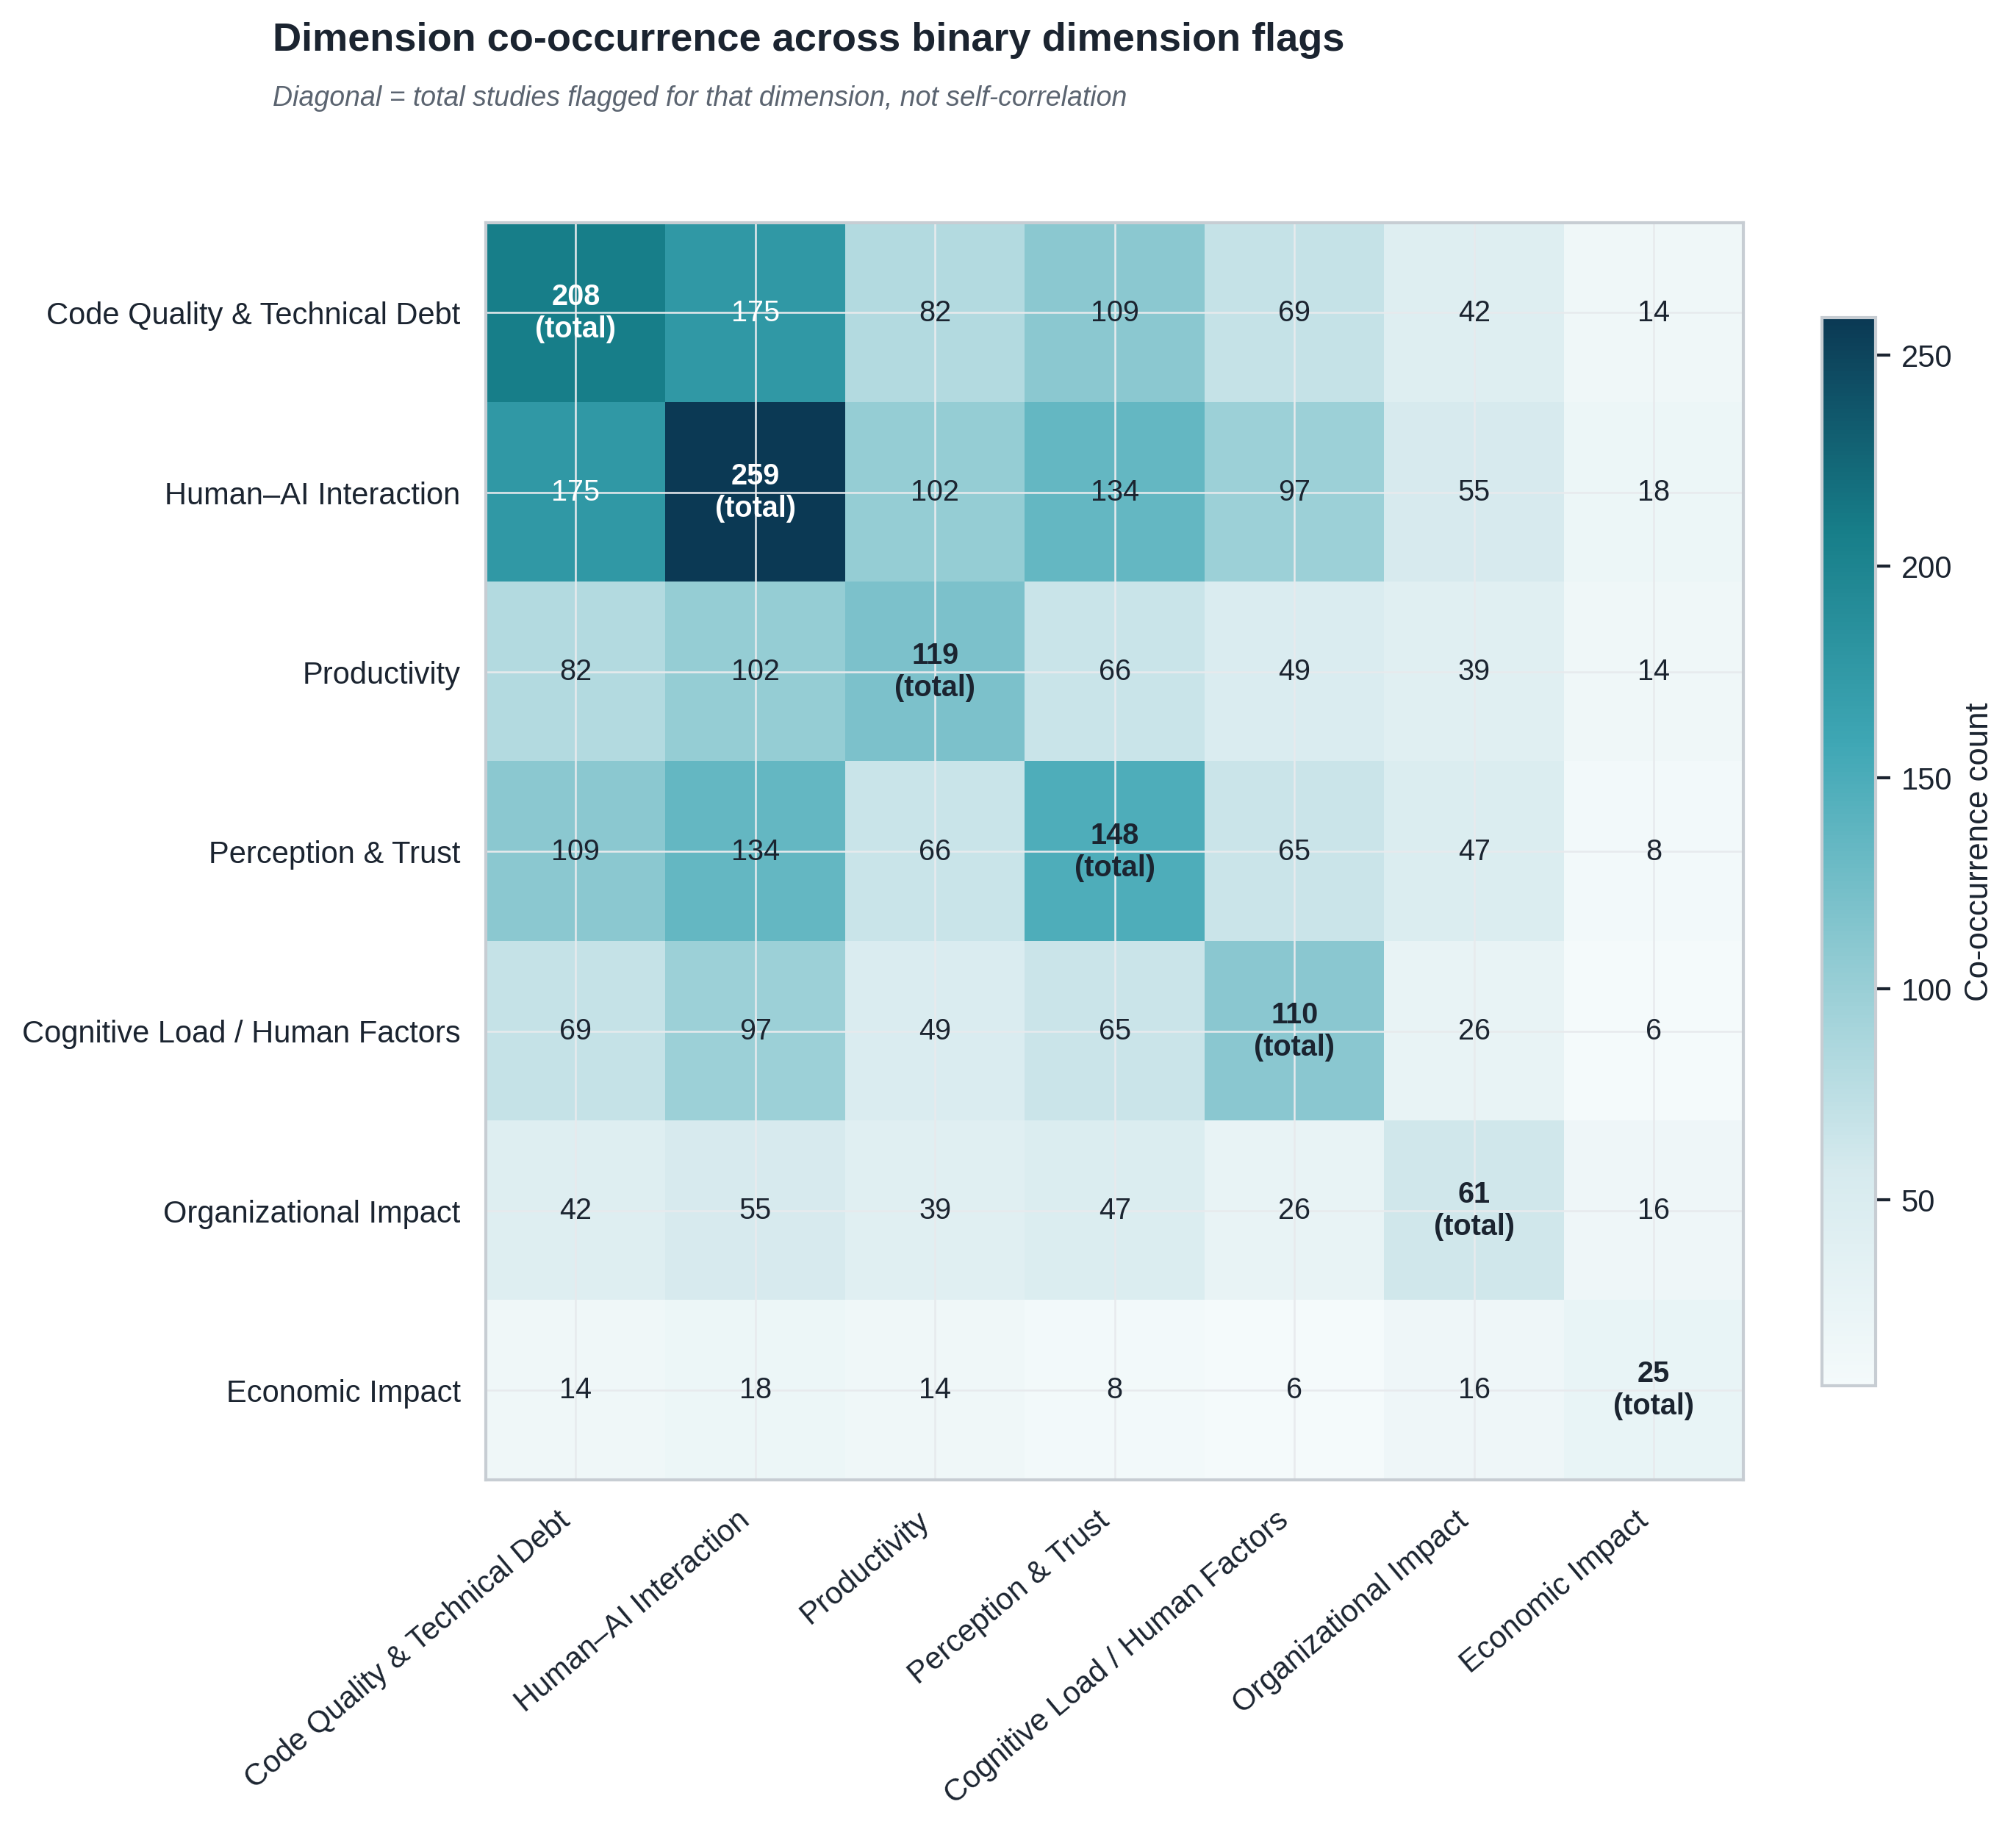
\includegraphics[width=0.82\linewidth]{figures/C1_dimension_cooccurrence.png}
    \caption{Dimension co-occurrence across binary dimension flags. The diagonal reports the total number of studies flagged for that dimension in any role, not self-correlation.}
    \label{fig:cooccurrence}
\end{figure}

This coupling is further reflected in how the methodological rigour of the corpus has evolved. As noted in Section~\ref{sec:corpus-profile}, the share of A1 (high-rigour) studies rose from 16.7\% in 2022 to 54.7\% in 2026 (Fig.~\ref{fig:quality_evolution}). This trend suggests that the field's growing empirical maturity has accompanied, rather than preceded, its conceptual shift toward treating code quality and human--AI interaction as a joint object of study: as researchers gained more rigorous tools for evaluating AI-generated code, the entanglement between technical reliability and interaction dynamics became increasingly visible in the evidence itself, reinforcing the socio-technical framing proposed in this paper rather than a purely technical one.

What the literature documents at the level of research design, organisations already confront at the level of deployment. CodeCompose's rollout to 16,000 engineers required acceptance monitoring, suggestion-level telemetry, and feedback loops precisely because generation and verification could not be separated once code reached shared repositories \cite{murali_ai-assisted_2024}, and the StackSpot AI case shows the same coupling from the opposite direction: a contextualised assistant only became useful once it was integrated with platform infrastructure, repository context, and organisational learning loops, none of which is a property of the underlying model itself \cite{pinto_lessons_2024}. Research-software adoption evidence extends this beyond commercial engineering: uptake depended on local norms and institutional support rather than on tool availability \cite{besser_how_2026}, and mixed-methods evidence on team-level collaboration shows that coordinating assistance and oversight is itself an organisational skill, not an automatic consequence of individual tool use \cite{stray_human-ai_2025}.

Read together with the role reconfiguration documented in Section~\ref{sec:disc-role-reconfiguration} and the governance argument developed in Section~\ref{sec:disc-security-governance}, the picture is consistent rather than coincidental: generation efficiency, verification overhead, interaction quality, trust calibration, and cognitive redistribution are not independent dials that organisations can adjust one at a time. They are coupled in the evidence base itself, and the organisations in this corpus that scale AI assistance successfully are, in effect, the ones that have built infrastructure around that coupling rather than around any single construct in isolation. This positions Organisational Impact not as one dimension among seven, but as the level at which the other six are jointly absorbed, tested, and either reconciled or left to accumulate as unrecorded cost. Whether that cost has in fact been recorded, and at what price, is the question the next section is forced to confront with the thinnest evidence base in the entire corpus.
% Discussion F ends here

% Discussion G starts here
\subsection{Economic Implications and Evidence Gaps}
\label{sec:disc-economic-gaps}
Section~\ref{sec:economic} already named Economic Impact as the aggregate expression of the whole socio-technical equilibrium: it is, in principle, the construct that would tell us whether the trade-offs documented throughout this Discussion, faster generation against verification overhead, competency investment against role disruption, governance cost against risk reduction, net out to a gain or a loss. It is also, by a wide margin, the part of the corpus least equipped to answer that question: Economic Impact accounts for a single primary study (0.3\% of the corpus; Section~\ref{sec:corpus-profile}), and that single study is the corpus's only entirely category-B dimension (Section~\ref{sec:corpus-profile}). The 25 studies appearing in the Economic Impact column of the dimension co-occurrence matrix (Fig.~\ref{fig:cooccurrence}) record secondary or proxy contributions to economic questions rather than primary Economic Impact designs; none treats cost-benefit analysis or return on investment as its principal research question. The construct the framework needs most is the one the evidence base can support least.

The proxy evidence assembled in Section~\ref{sec:economic} is a careful response to this constraint, not a substitute for it. Adoption-scale figures such as CodeCompose's 22\% suggestion acceptance and 8\% AI-authored changed code \cite{murali_ai-assisted_2024} show that AI-generated code is entering production at scale, but scale of adoption is not the same quantity as net cost or benefit. The hidden-cost evidence already discussed, validation labour in smart-contract generation \cite{karanjai_who_2023}, increased repair burden in constrained bug-fixing \cite{jesse_large_2023}, and 170 issues left unresolved by every evaluated agent in one study \cite{chen_evaluating_2024}, answers a narrower question than the one Economic Impact is meant to settle: each shows that a specific cost exists somewhere in the pipeline, not what that cost amounts to once netted against the time saved elsewhere. No study in this corpus performs that netting in a single design.

This is also the gap's precise methodological shape, not just its size. Cost-benefit evidence remains incomplete because productivity and correctness outcomes are essentially never measured in the same study, on the same tasks, as the validation, review, and remediation effort they generate; studies that gesture towards this connection, including the modification-effort and quality evidence discussed in Sections~\ref{sec:cqtd} and~\ref{sec:disc-meta-competencies}, measure a bounded piece of the cost without the matched baseline or accounting data that would let it be priced. What would close this gap is not more proxy evidence of the kind already available, but prospective, instrumented studies inside real software teams that track developer time, review load, test additions, defect escape, and downstream maintenance against a matched comparison condition, ideally using accounting data rather than self-report or task-level time trials.

The corpus contains exactly one attempt at this kind of study, and its limits illustrate why the gap persists. A FinTech total-cost-of-ownership comparison reports a lower unit cost for Copilot than junior-only staffing, with roughly 61\% return on investment and a payback period of about 7.4 months \cite{rodriguez_comparative_2025}. This is the right shape of evidence, a matched comparison grounded in accounting data, but it is a single peripheral, category-B case study from one company in one sector, and its very isolation in the corpus is itself a finding: across the five years of literature covered here (2022--2026; Section~\ref{sec:corpus-profile}), this is the only study that even attempts it.

This leaves the economic side of the socio-technical equilibrium framework structurally weaker than its technical and interactional sides, and that asymmetry is worth stating plainly rather than smoothing over. It is also likely to widen rather than narrow as the field moves towards the agentic systems discussed in the next section: the proxies and the lone primary study reviewed here describe single-shot generation and moderate-autonomy assistants, not the multi-agent configurations already shown, in this corpus, to trade longer reasoning trajectories and higher correction rates for no consistent gain over single-agent approaches \cite{yin_comprehensive_2025}. If compute and orchestration cost rise with autonomy while net benefit does not rise correspondingly, the evidence gap identified here is not a temporary lag behind a fast-moving field; it is a gap the field is currently moving away from closing.
% Discussion G ends here

% Discussion H starts here
\subsection{From Tools to Systems: Increasing Autonomy and Complexity}
\label{sec:disc-agentic} 
The competencies discussed in Section~\ref{sec:disc-meta-competencies} and the supervisory role documented in Section~\ref{sec:disc-role-reconfiguration} both implicitly assume a single point of contact between developer and output: one prompt, one generated artefact, one validation pass. Agentic systems break that assumption by inserting multiple autonomous decision points, retrieval, localisation, patch generation, repair, between the request and the result. The corpus is careful not to overstate what this changes: multi-turn interaction and agentic workflows do not monotonically improve code quality, and additional turns or additional autonomy have been shown to repair, preserve, or amplify defects depending on trajectory, with import-related errors decreasing only partially, from 48.3\% to 44.6\%, across successive conversational turns in one analysis \cite{zhong_developer-llm_2025}. What increasing autonomy adds is not simply more of the same trade-off documented throughout this Discussion; agentic patch evaluation across 4,892 patches from ten different coding agents found divergent modification patterns relative to gold-standard patches, showing that autonomy expands the surface area over which quality and security risk can manifest \cite{chen_evaluating_2024}, which changes the shape of the verification problem, not only its size.

That expansion has a specific, governance-relevant character. A benchmark reconstructing the exact repository state and natural-language requirement under which a human developer originally introduced a real vulnerability found that, across three popular code agents and five backbone language models, the best-performing combination produced output that was both functionally correct and free of the reconstructed vulnerability in only 23.8\% of cases; more importantly, an agent's likelihood of introducing a given vulnerability type was largely unrelated to how frequently that type occurred in the underlying training data \cite{chen_securevibebench_2026}, a pattern consistent with separately reported insecure-agentic-behaviour rates as high as 56.61\% depending on study and task setting \cite{kozak_when_2025}. This directly complicates the governance argument developed in Section~\ref{sec:disc-security-governance}. Review and audit practices naturally prioritise the vulnerability types known to be most common, but if an agent's risk profile is decoupled from base-rate frequency, that prioritisation strategy will systematically miss the risks agentic systems actually introduce. Governing agentic output may therefore require comprehensive review rather than risk-weighted review, a materially more expensive governance posture than the one Section~\ref{sec:disc-security-governance} described for single-shot generation.

Autonomy also fails in a second, less expected way: by coordinating, not by reasoning too little. A comprehensive comparison of seven general-purpose agent frameworks across software development, vulnerability detection, and program repair found that single-agent frameworks outperformed multi-agent frameworks on most tasks, with the multi-agent systems' longer reasoning trajectories and higher correction rates reflecting information loss and inter-agent error propagation rather than more thorough problem-solving \cite{yin_comprehensive_2025}. This is the sharpest available evidence for the non-monotonic turns-and-autonomy pattern already established in this corpus: orchestrating more agents is the most autonomy-intensive configuration studied here, and it is also the one that performs worst, not best, directly contradicting the intuitive assumption that distributing a task across more autonomous components should make it more reliable.

These two failure modes compound rather than offset one another. If validation increasingly means inspecting a multi-step trajectory rather than a single artefact (Section~\ref{sec:disc-meta-competencies}), and that trajectory is itself an unpredictable source of risk (above) produced by coordination failure rather than insufficient reasoning depth (above), then the supervisory role documented in Section~\ref{sec:disc-role-reconfiguration} becomes harder to discharge exactly as the corpus's capacity to characterise its economic cost (Section~\ref{sec:disc-economic-gaps}) remains thin. Increasing autonomy does not relax any of the tensions this Discussion has traced; it raises generation efficiency while raising verification overhead, governance cost, and economic uncertainty alongside it, not against it.

The clearest lesson from this evidence is therefore a caution against equating autonomy with progress along any single construct of the socio-technical equilibrium framework. Agentic evaluation is also the newest and least-replicated sub-literature considered in this study, which means the claims summarised here, more than those in any other section of this Discussion, are the ones most likely to be revised, qualified, or contradicted as further evidence accumulates, a possibility the next section examines directly.
% Discussion H ends here

% Discussion I starts here
\subsection{Convergence and Contradiction: Where the Corpus Agrees and Where It Does Not}
\label{sec:disc-convergence}
This Discussion has so far built a cumulative argument: that AI assistance reliably increases generation efficiency, that this efficiency is consistently offset by verification overhead in some form, and that interaction quality, trust calibration, cognitive redistribution, and organisational structure determine whether that offset is managed well or badly. It is worth being explicit about how solid this convergence actually is before turning to where the corpus disagrees. Disagreement in this literature takes three distinct forms, not one: a genuine contradiction, where studies measure substantially the same construct under comparable conditions and reach incompatible conclusions; a context effect, where apparent disagreement is explained by differences in task realism, benchmark design, or interaction governance; and an unresolved tension, where the corpus poses a real two-sided question without yet supplying the matched evidence needed to settle it. Most of what looks like disagreement in this corpus is the second or third kind. The realism gap between benchmark and repository-level performance, traced repeatedly throughout this Discussion (Sections~\ref{sec:disc-productivity-paradox} and~\ref{sec:disc-agentic}), is itself the clearest example of a context effect: a study contrasting 400 real-world classes against 100 synthetic benchmark classes found exactly this pattern, models that perform well on bounded synthetic tasks lose ground once class-level, real-world generation is required \cite{rahman_beyond_2025}, because bounded, single-shot tasks reward local synthesis, while repository-level, multi-step, security-sensitive tasks expose the same underlying models to integration debt and environmental fragility that bounded tasks do not surface. The corpus is not contradicting itself when one study reports high benchmark success and another reports substantial repository-level fragility; it is reporting the same underlying capability under two different measurement conditions.

The genuine contradiction in the corpus, the one disagreement that survives this filtering, concerns whether AI-generated code carries systematically higher security and maintainability risk than human-written code at repository scale. The case for elevated risk draws on production data: AI-authored commits tracked across a large repository sample showed code smells in 89.1\% of distinct technical-debt issues, with 24.2\% surviving to the latest revision \cite{liu_debt_2026}, and Copilot-generated snippets mined directly from GitHub projects have been found to carry identifiable security weaknesses \cite{fu_security_2025}. The case against treating this as categorically worse than human practice is just as direct: a study explicitly asking whether Copilot introduces vulnerabilities at a rate comparable to human developers reports a figure in the same broad range as the elevated-risk studies above, without establishing that a matched human baseline would score better \cite{asare_is_2024}, and a more recent study comparing GPT-generated code against real developer code drawn from authentic development interactions found no clear gap between the two: the LLM-authored snippets carried vulnerabilities at rates comparable to their human-written counterparts \cite{belozerov_secure_2026}. These are not papers asking different questions and talking past each other; they are largely asking the same question and reaching different answers, because each study operationalises the human-AI comparison differently, controlled-task baselines, mined GitHub history, or AI-authored commits identified after the fact, and matched repository-scale comparisons using a single, shared baseline definition remain rare. This is precisely why Section~\ref{sec:cqtd} phrased its own conclusion with care, that AI-generated code does not categorically outperform human-written code once security and maintainability are considered \cite{asare_is_2024,borg_echoes_2026}, a deliberately hedged claim rather than a resolved ranking, because the ranking itself is not yet resolved.

A second tension is unresolved rather than contradictory, and it complicates the governance argument made in Section~\ref{sec:disc-security-governance} from a different angle than the agentic evidence in Section~\ref{sec:disc-agentic} did. Targeted prompt design has been shown to reduce insecure code generation and raise secure-code rates substantially \cite{res_enhancing_2024}, repair-oriented prompting interventions report meaningful security-patching success \cite{alrashedy_can_2024}, and structured prompting and role strategies have been shown to improve vulnerability detection and classification across multiple programming languages, with one practitioner-facing tool doubling detection accuracy in a study with professional developers \cite{dozono_large_2026}. Set against this, large-scale security evaluations covering thousands of generated snippets continue to find substantial vulnerability rates under realistic conditions \cite{siddiq_generate_2023,pearce_asleep_2025}, and insecure agentic behaviour persists at rates that vary widely by study and task setting \cite{kozak_when_2025}. Both sets of findings can be true at once: prompt engineering is a genuine mitigation mechanism in the studies that test it directly, and it is also, in the corpus considered as a whole, a fragile one whose benefits have not been shown to transfer reliably across languages, model versions, and vulnerability classes. What is missing is not more evidence that prompting can help in principle, that point is now well established, but controlled comparisons of the same prompt families across the same tasks, vulnerabilities, and models, which would establish a dose-response relationship rather than a list of cases where it worked. Until that evidence exists, the governance recommendation in Section~\ref{sec:disc-security-governance}, formalise the techniques already shown to work, needs the qualification that "shown to work" currently means shown to work in the specific study that tested it, not shown to generalise.

A third tension sits directly underneath the agentic evidence discussed in Section~\ref{sec:disc-agentic}: does agentic capability, the ability to test, revise, and repair across multiple steps, make code safer than single-shot generation, or does it accumulate new exposure that single-shot studies cannot see? Repair-oriented evidence supports the safer reading: agentic patching has produced measurable issue-resolution rates on real-world benchmarks \cite{aleithan_swe-bench_2024}, and structured repair prompting reports meaningful security-patching success \cite{alrashedy_can_2024}. Risk-oriented evidence supports the opposite reading: insecure agentic behaviours have been observed at rates reaching the upper end of the figures already discussed in Section~\ref{sec:disc-agentic} \cite{kozak_when_2025}, dependency-gap analysis of agentic coding output finds reproducibility failures that single-shot generation studies are not designed to detect \cite{vangala_ai-generated_2026}, and a repository-level security benchmark explicitly designed to mirror real AI-assisted programming scenarios found that a larger reasoning budget did not reliably translate into more secure code, complicating any simple story in which more deliberation or more autonomy straightforwardly improves outcomes \cite{lian_ase_2025}. The two anchors developed in Section~\ref{sec:disc-agentic}, the finding that an agent's likelihood of introducing a given vulnerability type is unrelated to that type's frequency in training data, and the finding that multi-agent orchestration underperforms single-agent approaches because of inter-agent error propagation rather than insufficient reasoning, are best read as recent, sharp data points inside this still-open tension rather than as its resolution. They show that more autonomy does not straightforwardly buy more safety, but the corpus has not yet produced the paired single-shot-versus-agentic comparisons, holding model, task, and security criteria constant, that would settle the question either way.

A fourth tension is less about risk than about measurement: whether model rankings are stable enough to support general claims about which tool is "best." Some comparative evaluations support a rankable hierarchy, at least within a given benchmark: a six-model comparison on the HumanEval benchmark found one frontier model achieving the highest Pass@1 success rate by a clear margin over its closest competitor \cite{bayram_comparative_2025}, and a broader trustworthiness evaluation framework spanning 26 models likewise finds substantial, measurable performance variation across coding tasks \cite{gao_treat_2025}. Other comparisons reverse or flatten this picture once the task changes: on the same 18-task set, GitHub Copilot, BingAI, and ChatGPT produced markedly different solve rates \cite{idrisov_program_2024}, and separate comparisons of ChatGPT, Codeium, and Copilot \cite{ovi_benchmarking_2024} and of four AI-based assistants generating Java methods \cite{corso_generating_2024} likewise find that whichever tool ranks first depends on the specific task and language under test, not on a single underlying capability ordering. This is a context effect rather than a contradiction: the corpus supports local rankings within a fixed benchmark, language, and task type, but not a single global hierarchy of code-generation tools, and the practice followed throughout this Discussion, citing specific figures from specific studies rather than asserting that one tool is unconditionally superior, reflects this constraint rather than stylistic caution.

These tensions, and others not detailed here, developer expertise as a moderator rather than a uniform amplifier or leveller of outcomes, and whether AI-specific technical debt is qualitatively distinct from ordinary maintainability debt, share a structure rather than a cause. None of them is resolved by collecting more of the same kind of evidence; each requires a different kind of study than the corpus currently has in volume: matched human-AI repository comparisons, controlled prompt-family comparisons, paired single-shot-and-agentic designs, and rankings reported within a single, fixed evaluation frame rather than across incompatible ones. The corpus's own trajectory gives some reason for optimism here: the share of high-rigour studies in this evidence base rose from 16.7\% to 54.7\% between 2022 and 2026 (Section~\ref{sec:disc-organisational}), and these are exactly the kinds of matched, controlled designs that more rigorous methodology tends to produce. But as of the cutoff for this review, the tensions documented above remain open, and the synthesis offered in the preceding sections of this Discussion should be read accordingly: as the corpus's best-supported account given the comparator designs currently available, not as a set of settled facts immune to revision. What this conditional-validity pattern, disagreement tracking what is measured rather than whether AI assistance helps or hurts, implies for the socio-technical equilibrium framework itself, rather than for any single empirical claim, is the question the next section turns to directly.
% Discussion I ends here

% Discussion J starts here
\subsection{Theoretical Implications: Revisiting the Socio-Technical Equilibrium Framework}
\label{sec:disc-theoretical}
Section~\ref{sec:disc-convergence} traced where the corpus agrees and where it does not, and closed by asking what that pattern, conditional validity rather than either convergence or contradiction, means for the socio-technical equilibrium framework itself rather than for any single empirical claim. This section takes up that question directly. The framework names five constructs: generation efficiency, verification overhead, interaction quality, trust calibration, and cognitive redistribution (Fig.~\ref{fig:framework}). Having used these constructs to organise eight subsections of empirical synthesis and one subsection of explicit disagreement, it is now possible to ask a sharper question than whether the framework is broadly consistent with the evidence: which construct does which theoretical work, where does the framework need qualification, and does it survive the strongest available readings of the corpus that would replace it with something simpler?

\begin{figure}[h]
    \centering
    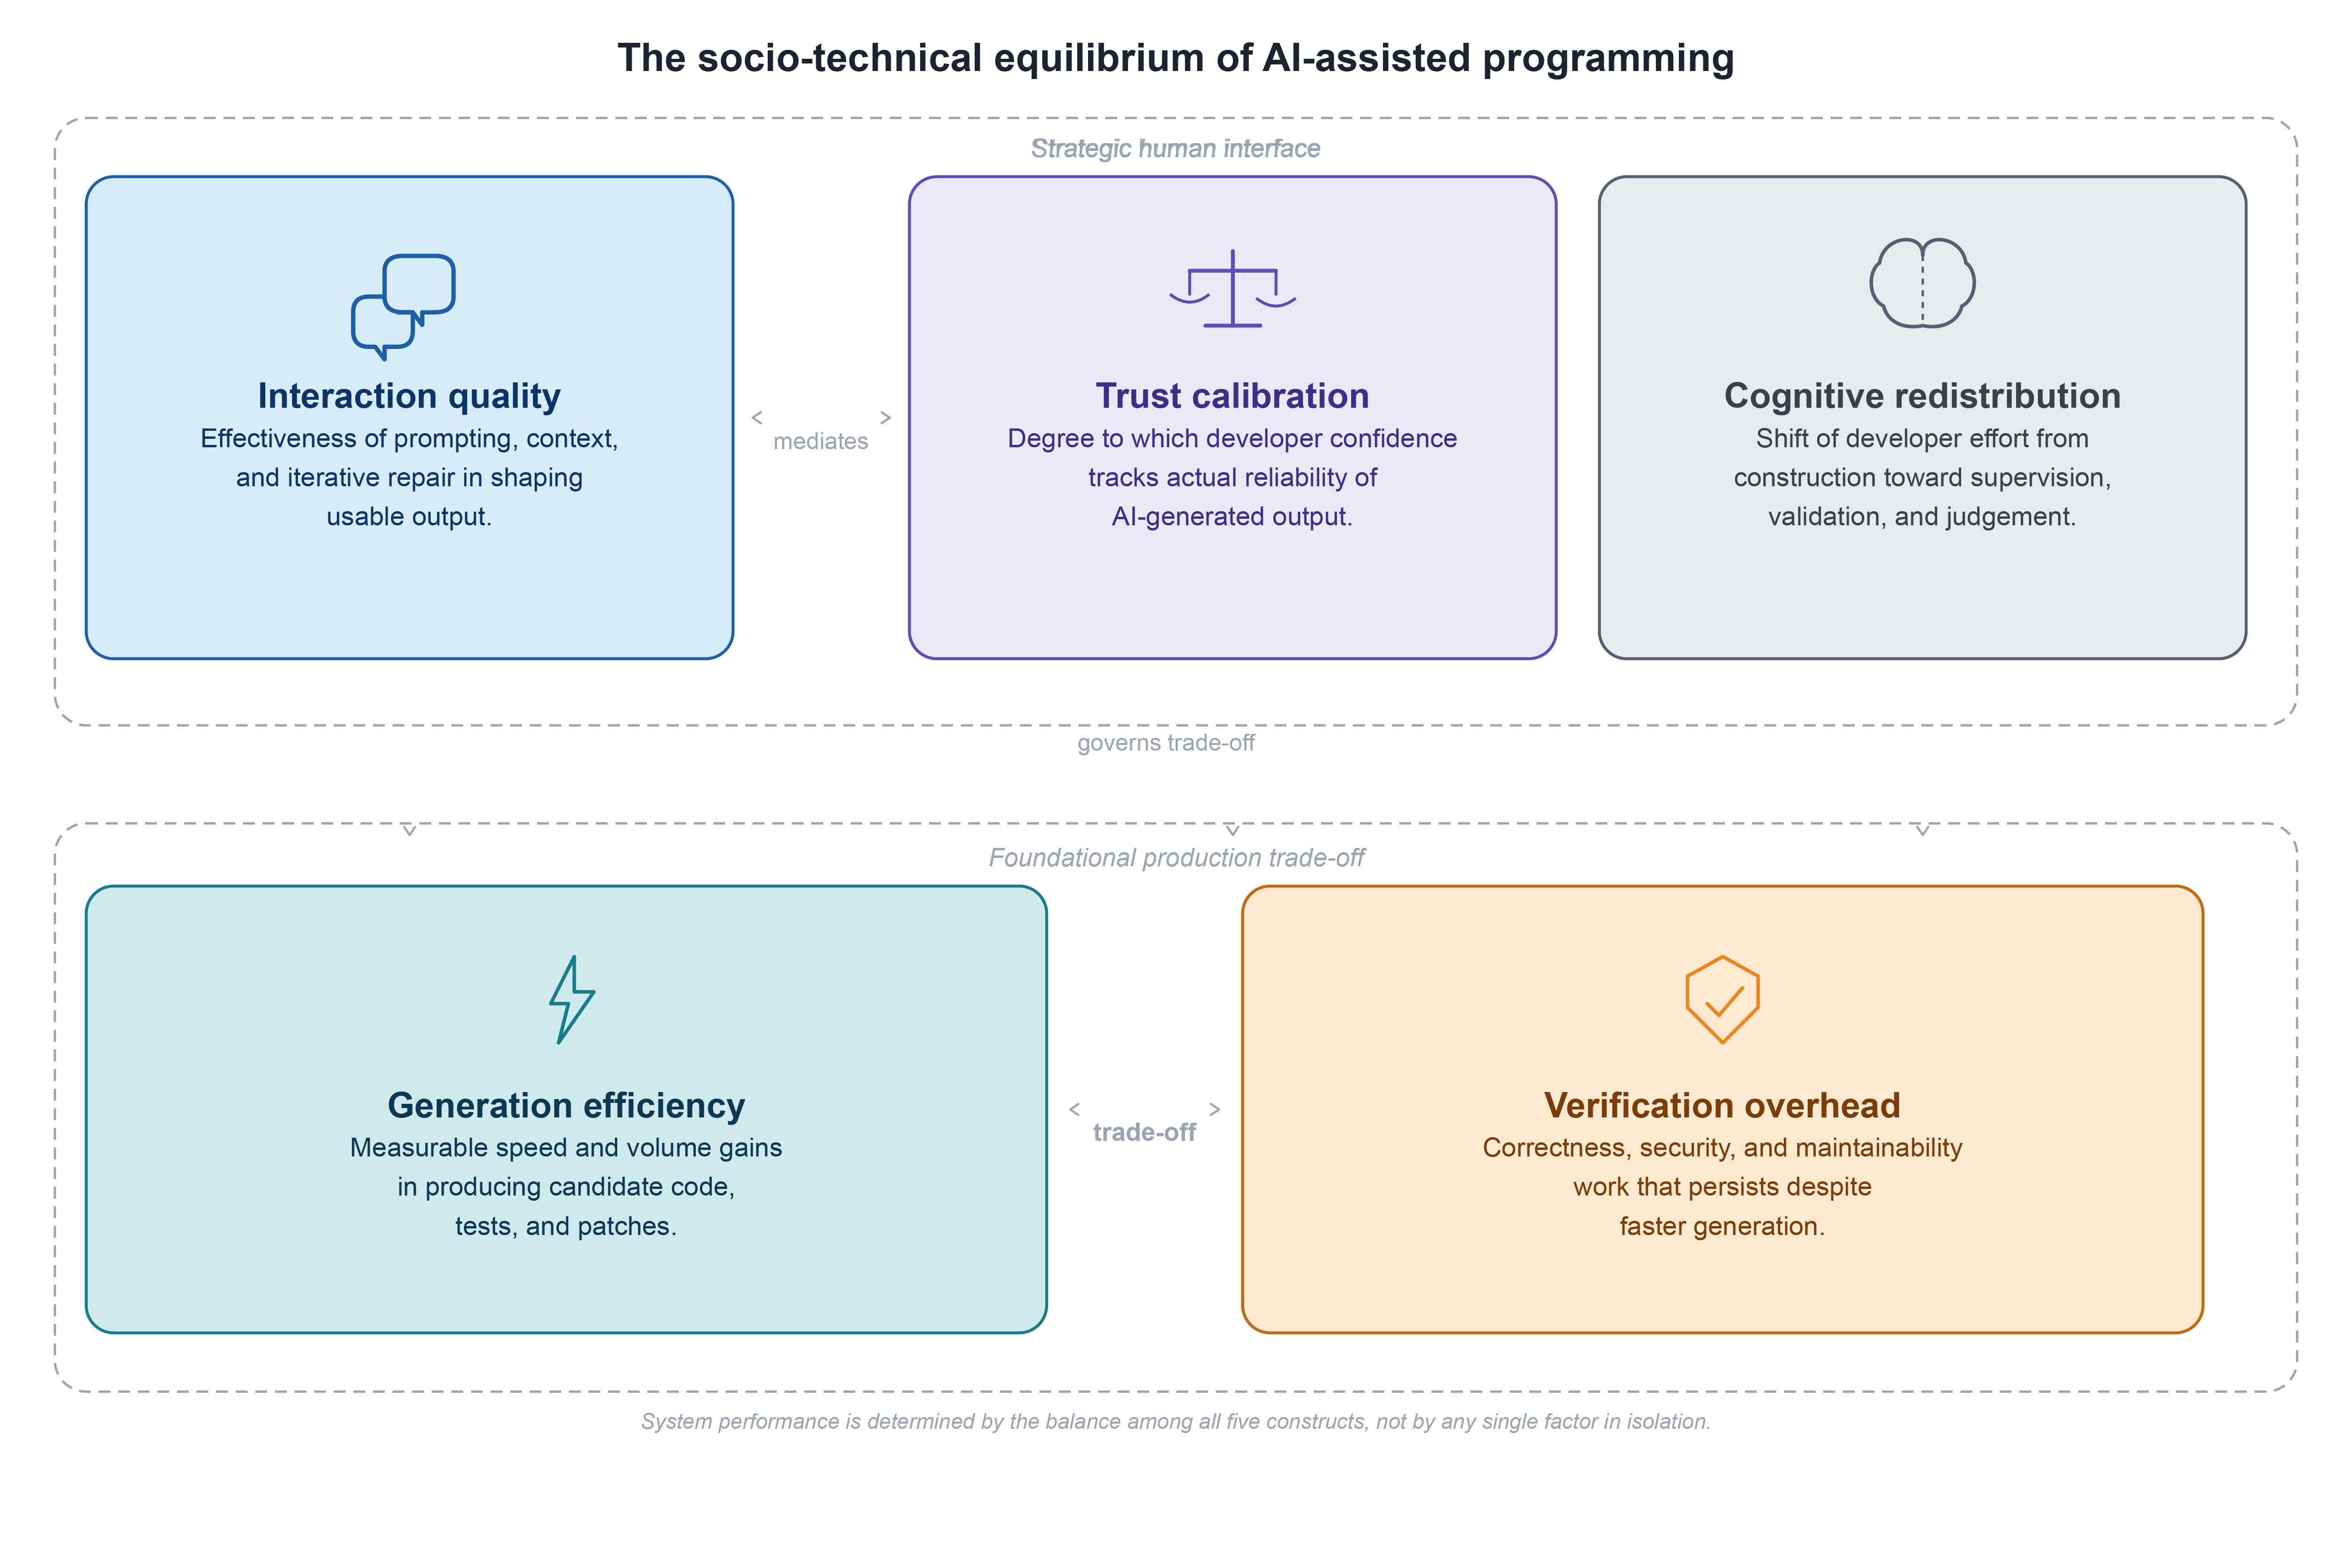
\includegraphics[width=0.95\linewidth]{figures/fig_framework.png}
    \caption{The socio-technical equilibrium framework. The five constructs
    are organised in two tiers: the foundational production trade-off between
    generation efficiency and verification overhead (below), and the strategic
    human interface through which interaction quality, trust calibration, and
    cognitive redistribution govern how that trade-off is absorbed (above).
    Amber flags verification overhead as the primary risk construct.}
    \label{fig:framework}
\end{figure}

The first refinement this Discussion supports is that the five constructs are not five independent variables doing the same explanatory work; they specialise, and the corpus's own structure already hints at why. The two dimensions most clearly anchoring verification overhead on one side, and interaction quality and trust calibration on the other, code quality and technical debt, and human-AI interaction, are also the two dimensions that co-occur most often in the corpus, appearing together in 175 studies, the single largest off-diagonal cell in the dimension co-occurrence matrix (Section~\ref{sec:disc-organisational}). This is not a coincidence the framework merely accommodates after the fact; it is the pattern a framework treating these constructs as causally linked, rather than as alternative descriptions of the same outcome, should produce. The evidence marshalled throughout the preceding five subsections (\ref{sec:disc-productivity-paradox}--\ref{sec:disc-security-governance}) and Section~\ref{sec:disc-convergence}, security vulnerability rates that hold up across very different study designs, repository-scale technical debt that survives well past initial generation, and a productivity paradox that recurs whenever speed is measured without measuring validation, anchors verification overhead as a structural, near-mechanical consequence of generation efficiency: faster candidate production does not by itself resolve correctness, security, or maintainability, and nothing in this corpus shows local functional success reliably predicting those properties without independent checking. Interaction quality and trust calibration do different theoretical work. They do not determine whether verification overhead exists; they determine whether it is absorbed productively or compounds into hidden risk. An explicit cost model of AI-assisted programming makes this mechanism concrete: developers spend the majority of their interaction time, 51.5\% in one study, on AI-related activities rather than independent construction, with verification alone accounting for 22.4\% and suggestion acceptance running at only around 34\% (Section~\ref{sec:cognitive-load}) \cite{mozannar_reading_2024}, a direct empirical demonstration that the value of a generated suggestion depends on the cost of reading, understanding, and repairing it, not on how quickly it appears. Generation efficiency creates the overhead; interaction quality and trust calibration govern what happens to it next.

Cognitive redistribution occupies a third theoretical position in this structure: it is not a mechanism that creates or governs the trade-off, but its most directly observable marker, the shift of developer effort from construction to supervision that this Discussion has traced from the prompting and validation competencies in Section~\ref{sec:disc-meta-competencies} through to the reconfigured developer role in Section~\ref{sec:disc-role-reconfiguration}. That section's strongest contribution to the framework, however, is one the framework as originally specified does not yet have a formal place for: redistribution is not evenly experienced. AI Skill Threat was reported at higher rates among racially minoritised developers, who also rated AI-assisted output quality lower than their peers, and reported upskilling intent was lower among women and LGBTQ+ developers (Section~\ref{sec:disc-role-reconfiguration}). A framework that treats cognitive redistribution as a uniform shift in where effort is spent, without a construct for how unevenly that shift lands across the developer population, is currently under-specified relative to its own evidence base. This is not a failure of the framework so much as the clearest single refinement this Discussion identifies: cognitive redistribution should be read as differentially distributed, not as a uniform property of the workforce undergoing it.

Tested against rival readings, the framework holds most clearly where it is needed most. A purely technocratic reading, that AI-assisted programming is fundamentally a productivity and capability story and that socio-technical framing overstates the complexity, cannot accommodate the single most load-bearing finding in this Discussion: experienced developers in a controlled field experiment took 19\% longer to complete real tasks with AI assistance despite forecasting a 24\% speed-up beforehand and believing afterwards that they had been 20\% faster (Section~\ref{sec:disc-productivity-paradox}). Capability and cost do not appear in different studies that a technocratic reading could simply prefer; they appear in the same study, the same developers, the same tasks. A purely pessimistic reading, that the evidence is mainly a story of deskilling and accumulating debt, fares no better: it cannot accommodate the demonstrated cases in which targeted prompt design, structured repair techniques, and interpretability tooling measurably improved outcomes (Section~\ref{sec:disc-security-governance}), nor the evidence that productivity loss is not universal but concentrated in specific tasks, populations, and interaction patterns (Section~\ref{sec:disc-human-factors}). Neither pole fits; the equilibrium framing pre-empts both. The framework also survives the objection that this corpus is simply too heterogeneous to unify under one theory, provided it is read as the mid-range theory it has been built as throughout, not as a universal law. Section~\ref{sec:disc-convergence}'s own conclusion is the direct evidence for this: disagreement across the corpus tracks what is measured, snippet, method, patch, repository, agent trajectory, far more than it tracks whether AI assistance helps or hurts in the abstract, and explaining patterned variation rather than asserting a single pooled effect is precisely what a mid-range framework is for.

The framework's most serious limitation is not theoretical but temporal, and this Discussion has already conceded it piecemeal rather than holding it back for this section. Economic Impact remains the corpus's thinnest and least rigorous dimension, composed of proxy evidence and a single peripheral case study (Section~\ref{sec:disc-economic-gaps}); agentic and multi-agent evidence is, by this corpus's own account, its newest and least-replicated sub-literature (Section~\ref{sec:disc-agentic}); and the specific percentages used throughout this Discussion, vulnerability rates, acceptance rates, repair-success rates, are tied to model generations and benchmark designs that will date quickly. None of this is fatal to the framework, but it does fix what kind of claim the framework can responsibly make. The durable claim is not that any specific figure cited in this Discussion will hold in two years' time; it is that generation efficiency will continue to create verification overhead, and that interaction quality and trust calibration will continue to determine whether that overhead becomes governed engineering work or accumulated, hidden risk, regardless of which model generation is doing the generating. Capability shifts the equilibrium point; it does not remove the need to ask where that point currently sits. This is also why this Discussion has been careful, particularly in Sections~\ref{sec:disc-economic-gaps} and~\ref{sec:disc-convergence}, not to pool incompatible percentages into a single effect size: measurement infrastructure, benchmark realism, and comparator choice are themselves part of the socio-technical system being described, not noise to be averaged away from it.

What this Discussion supports, after testing the framework against the corpus's own internal disagreements and against its strongest rival readings, is therefore a qualified version of the claim with which this Discussion began: AI-assisted programming does not settle into a single, stable state of higher or lower productivity, quality, or trust. It settles into different equilibria depending on whether generation efficiency is matched by adequate verification capacity, whether interaction quality and trust calibration are actively designed for or left to develop informally, and whether the resulting redistribution of cognitive work is recognised as something that lands unevenly across the people doing it. Security, examined directly in Section~\ref{sec:disc-security-governance}, remains the sharpest available test of this claim, because it is the one place in the corpus where every construct in the framework is implicated at once and where the cost of a poorly managed equilibrium is most concrete. The constructs this Discussion has used to organise eight sections of synthesis and two of explicit testing therefore stand, not as a finished theory of AI-assisted programming, but as the most defensible mid-range account this corpus currently supports of how that programming actually unfolds.
% Discussion J ends here

% Discussion ends here

% Threats to Validity starts here
\section{Threats to Validity}
\label{sec:threats}

As with any systematic literature review, the findings reported here are subject to limitations that should be considered when interpreting them. The threats below proceed from those bearing most directly on data collection and classification towards those bearing on synthesis and on the temporal scope of the evidence base itself.

First, the dataset includes a proportion of preprint studies that may not have undergone full peer review, which could affect the reliability of some findings. As shown in Fig.~\ref{fig:item_type}, preprints account for 38.8\% of the corpus (n=121), followed by conference papers (31.1\%, n=97), journal articles (27.9\%, n=87), theses (1.9\%, n=6), and a single book section (0.3\%, n=1). However, these studies were evaluated using the same structured quality-assessment framework described in Section~\ref{sec:quality-assessment}, which mitigates this risk by weighting conclusions toward CORE and A1/A2 evidence rather than publication venue alone.

\begin{figure}[h]
    \centering
    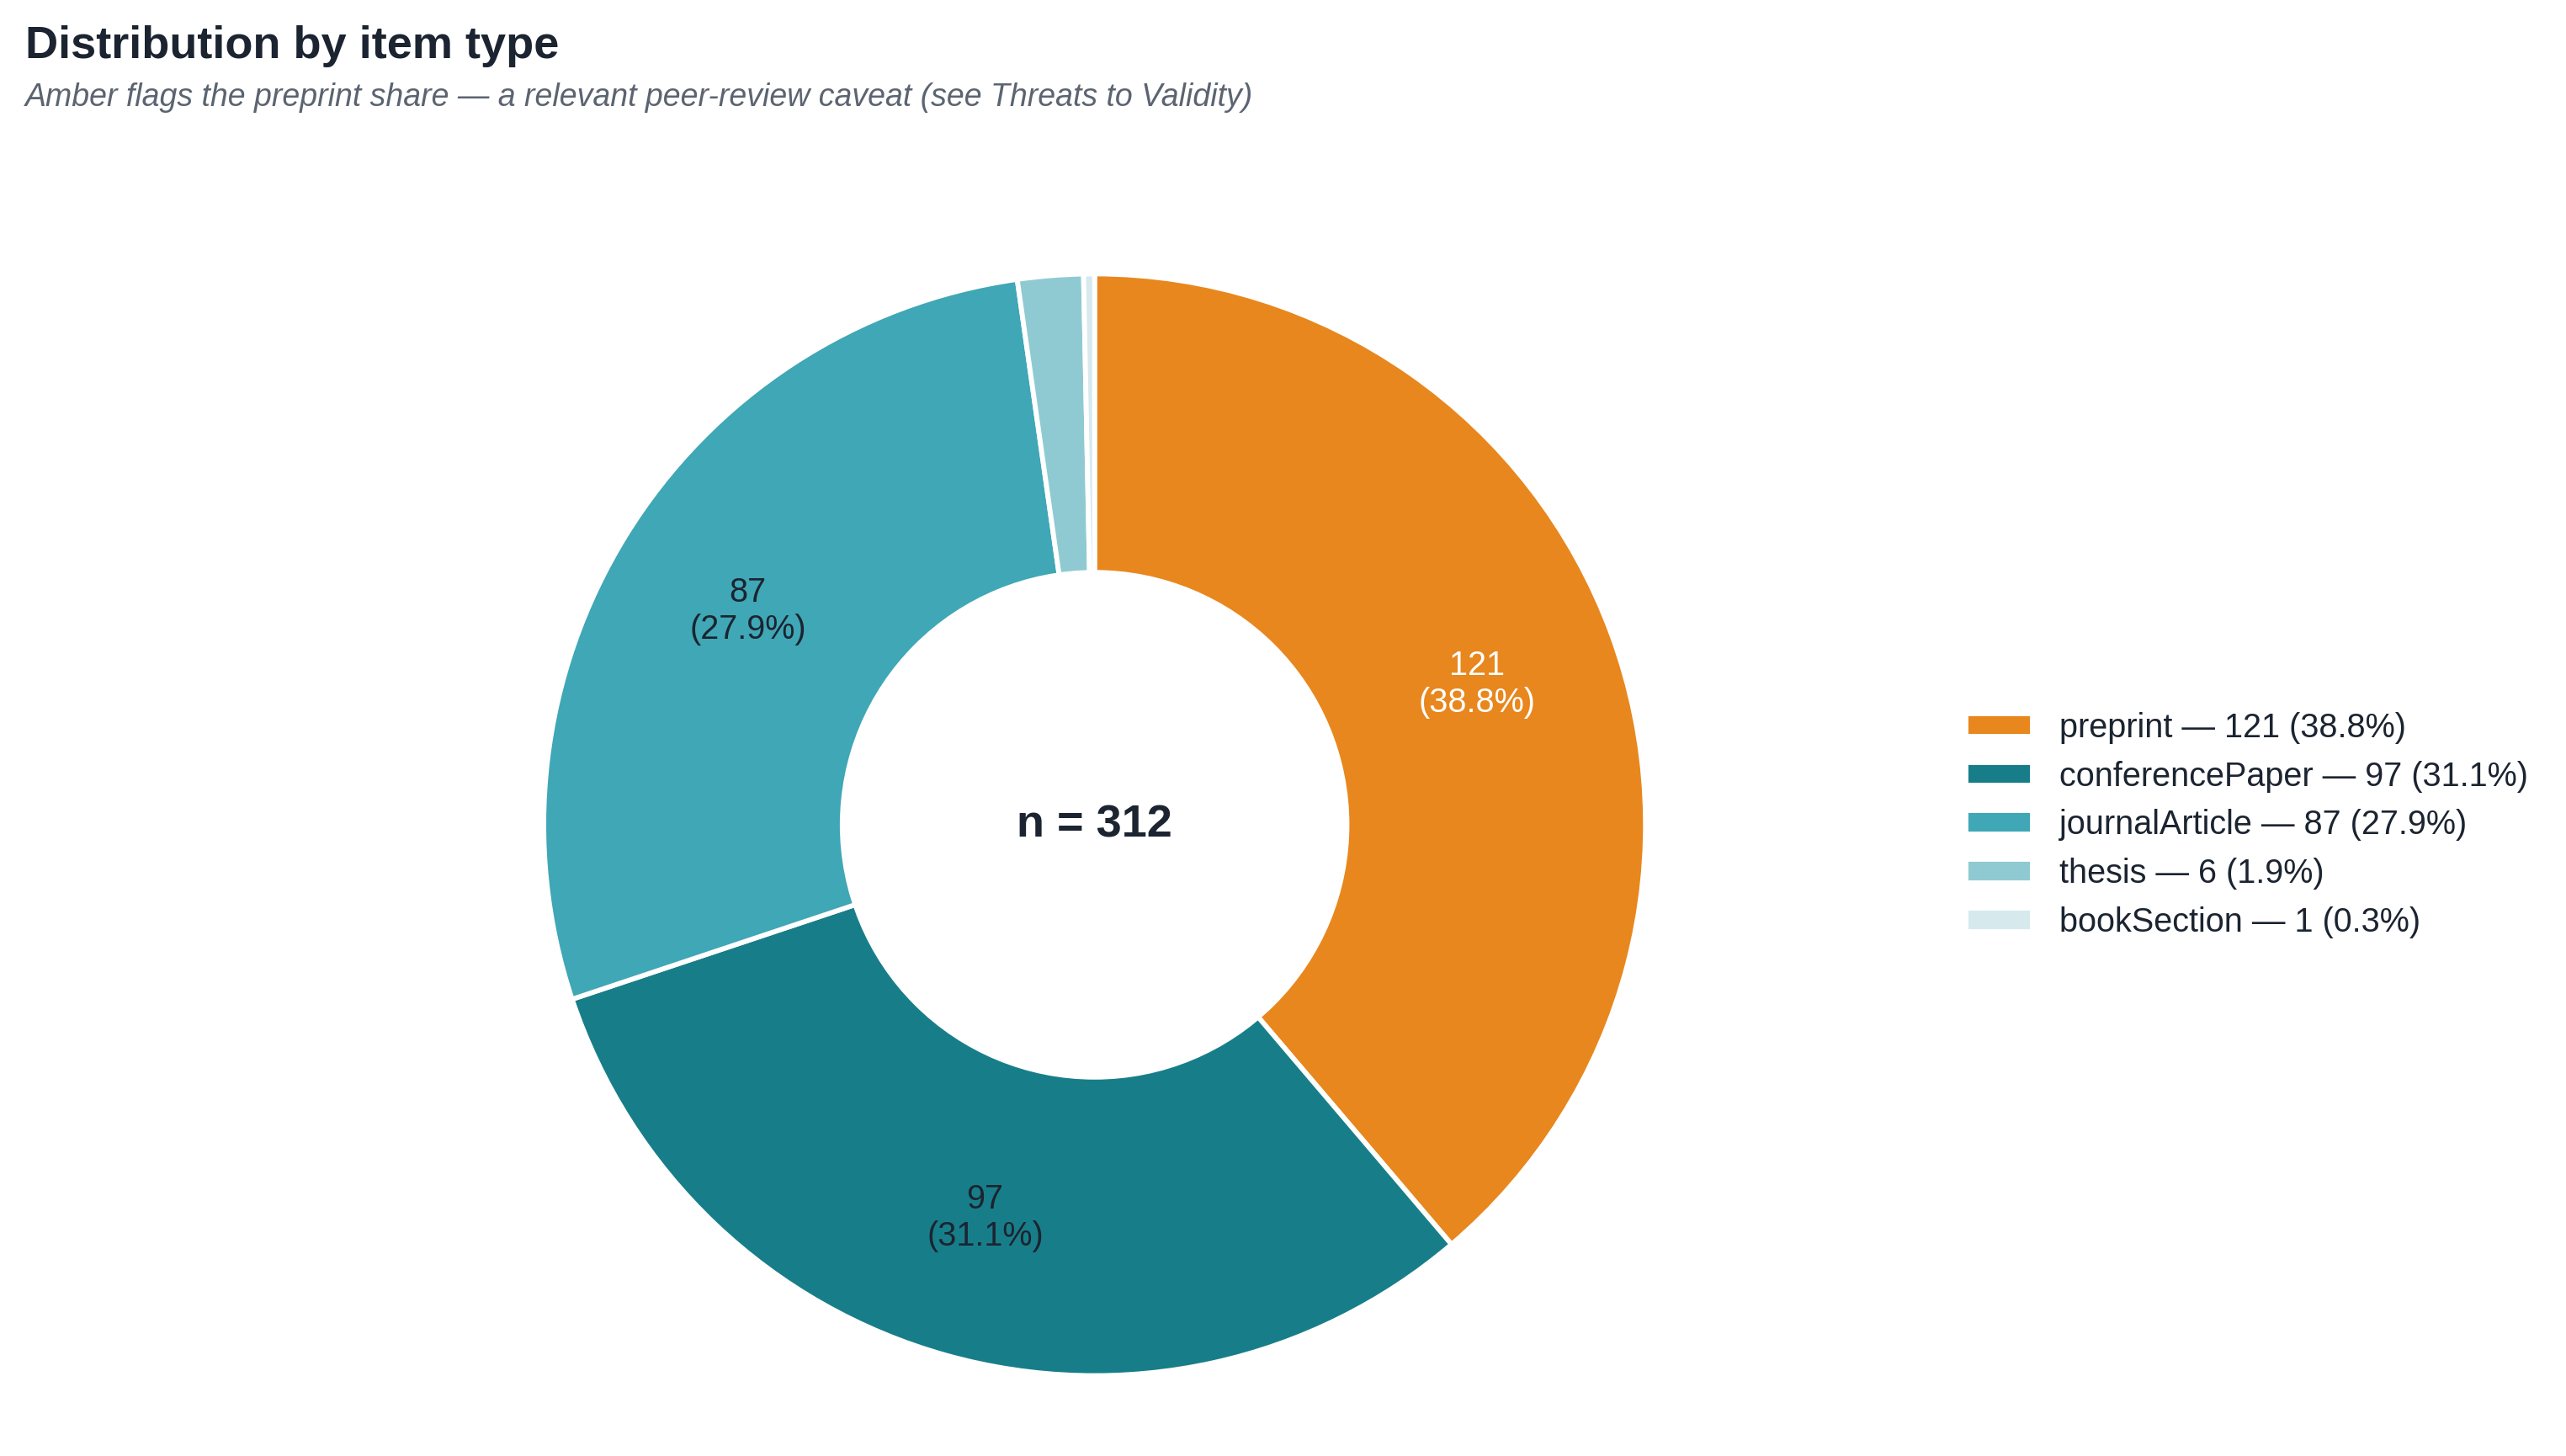
\includegraphics[width=0.82\linewidth]{figures/A3_item_type_distribution.png}
    \caption{Distribution of the corpus by item type. Amber flags the preprint share, the relevant peer-review caveat discussed here.}
    \label{fig:item_type}
\end{figure}

Second, this review was conducted by a single author, and screening, eligibility, and quality-classification decisions were therefore not cross-checked by an independent second rater; no inter-rater reliability statistic, such as Cohen's kappa, is reported. This is a standard limitation of single-author systematic reviews. It was partially mitigated by applying one structured evaluation protocol consistently across the full corpus and by running the classification process through multiple validation passes rather than a single pass (Section~\ref{sec:methodology}). A related, narrower threat concerns the small number of corpus studies published in Chinese, Russian, and German, which the author does not read directly; for these, AI-assisted translation supported reading and eligibility assessment under the same inclusion criteria applied to studies read directly in English, Spanish, and Portuguese. Interpretive nuance in the translated text could not be cross-checked against the author's own command of the source language, although this affects only a small fraction of the corpus.

Third, AI-assisted tools supported parts of the review process, and their use carried its own risk of error that required active mitigation rather than passive trust. Three tools were used: NotebookLM for corpus-wide thematic exploration and descriptive characterisation; ChatGPT (4o/o1 family) for single-paper deep extraction and scaffolding artefacts; and Elicit, in a limited pilot, for cross-validation of selected quantitative extractions. A dedicated pilot validation phase, conducted before the bulk of the extraction work, identified concrete failure modes in this usage. NotebookLM's retrieval occasionally conflated a paper's own empirical finding with a citation that paper made to a third-party source, at a measured rate of 12.4\% of rows in one pilot extraction; it also used an inline numbering scheme inconsistent with its own references list, and on one occasion silently omitted a paper from a structured extraction without flagging the omission. ChatGPT, without explicit safeguards, was separately observed to extract bracketed reference numbers as if they were quantitative findings, and to lose the grammatical subject of a sentence when splitting multi-figure sentences into separate extracted rows. These behaviours were mitigated by replacing pre-built reports with explicitly safeguarded prompts that instructed each tool not to report citation-derived figures, reference-cluster numbers, or unattributed subjects; by manual cross-validation of every structured extraction against the corpus list; and by cross-checking quantitative findings against single-paper deep extractions produced under these safeguards, which reduced detectable misattribution to near zero on spot-checks. Every quantitative figure cited in this manuscript was manually verified against its original source PDF prior to inclusion. The complete tool-by-tool audit and validation protocol, including measured error rates per tool and per phase, are documented in supplementary material.

Fourth, the heterogeneity of study designs, evaluation metrics, and experimental contexts across the corpus precluded a formal quantitative meta-analysis (Section~\ref{sec:methodology}). The structured synthesis approach adopted instead, combining frequency-based aggregation with qualitative pattern identification, is consistent with established systematic-review practice under high methodological variability, but it means that the percentages and ranges reported throughout this paper should be read as descriptive of the evidence base rather than as pooled effect-size estimates with an associated confidence interval.

Fifth, the corpus is bounded in time, spanning 2021 to 2026, in a field whose underlying tools and model generations change faster than a single review cycle. This temporal boundary was already identified in the Discussion (Section~\ref{sec:disc-theoretical}) as the socio-technical equilibrium framework's most serious qualification rather than a peripheral caveat: the specific figures reported throughout this paper are tied to the model generations and benchmark designs current at the time of writing, and should be expected to date more quickly than the underlying mechanisms they illustrate.

Despite these limitations, the combination of a dual-pathway search strategy, a documented and audited AI-tool validation protocol, consistent quality classification across the full corpus, and a sensitivity analysis confirming that supplementary-discovery records do not materially alter the corpus's empirical profile (Section~\ref{sec:methodology}) provides a defensible foundation for the synthesis presented in this review.
% Threats to Validity ends here

% Conclusion starts here
\section{Conclusion}
\label{conclusion}

This study set out to answer a single question: what is the impact of AI-assisted programming on software development processes and outcomes? Drawing on a corpus of 312 empirical studies spanning seven analytical dimensions, productivity, code quality and technical debt, human--AI interaction, cognitive load, organisational impact, economic impact, and perception and trust, the answer this review supports is neither uniformly positive nor uniformly cautionary. AI-assisted programming reliably accelerates the generation of code, tests, and patches; it does not, by itself, accelerate the slower and more distributed work of establishing that what was generated is correct, secure, maintainable, and fit for purpose. The clearest single illustration of this remains the productivity paradox that opened the Discussion: experienced developers who took longer to complete real tasks with AI assistance than without it, despite having forecast, and later believed, the opposite \cite{becker_measuring_2025}, a result this review reads not as an anomaly but as the visible edge of a much broader pattern.

That pattern is what this study has formalised as a socio-technical equilibrium: AI-assisted programming does not settle into a single, fixed level of productivity, quality, or trust, but into different equilibria depending on how generation efficiency and verification overhead are balanced, on whether interaction quality and trust calibration are designed for or left informal, and on how the resulting redistribution of cognitive work is recognised and managed. Tested against the corpus's own internal disagreements and against the strongest rival readings available, technocratic, pessimistic, anti-theoretical, and temporally sceptical, this framework held best as a mid-range account of patterned variation rather than as a universal law, with its most serious qualification being temporal: the figures reported throughout this review are tied to model generations and benchmark designs that will date, even as the underlying mechanisms they illustrate are likely to persist.

For practitioners and organisations, this account has direct implications. Productivity should be measured as validated, maintained output rather than as generation speed alone, since the gap between the two is precisely where this review's evidence concentrates. Prompting and validation literacy should be treated as a professional competency requiring deliberate development, not an incidental skill assumed to come bundled with tool access. Security and governance cannot be left to individual developer vigilance, since the evidence reviewed here shows confidence and risk moving in opposite directions under exactly the conditions where vigilance matters most; the same caution extends with greater force to agentic and increasingly autonomous systems, where the kind of risk introduced is not reliably predictable from how common that risk is elsewhere. Organisations that have absorbed these tensions successfully are not the ones that adopted AI assistance fastest, but the ones that built repositories, review routines, and competence models around it before scaling its use, and that recognised the resulting reconfiguration of the developer role as a transition some developers are better positioned to make than others.

The evidence base also has clear limits that should shape the research agenda rather than be treated as a footnote. Economic Impact remains the thinnest dimension in this corpus, and the field needs prospective, instrumented studies that price validation, remediation, and governance costs against accounting data rather than task-level proxies. Agentic and multi-agent evidence is the newest and least-replicated sub-literature reviewed here, and paired single-shot-versus-agentic designs, held constant on model, task, and security criteria, are needed before its place in the equilibrium can be stated with confidence. The equity dimension of cognitive redistribution, the finding that this shift in where developer effort is spent lands unevenly across racial, gender, and accessibility lines, is supported by early evidence that deserves dedicated longitudinal attention rather than a single passing citation. And several of the tensions catalogued in this review's own internal disagreement mapping, the comparative risk of AI-generated and human-written code at repository scale chief among them, will not be resolved by accumulating more of the same kind of study, but require matched designs built specifically to settle them.

AI-assisted programming, on the evidence synthesised here, is not a technology that automates software development so much as one that redistributes it, shifting the locus of developer effort, professional risk, and organisational responsibility rather than removing any of them. Whether that redistribution becomes durable engineering value or accumulated, hidden cost is not a property of the tools themselves, but of how deliberately the humans and organisations using them choose to manage the balance.
% Conclusion ends here

%\begin{acknowledgements}
%If you'd like to thank anyone, place your comments here
%and remove the percent signs.
%\end{acknowledgements}


% Authors must disclose all relationships or interests that 
% could have direct or potential influence or impart bias on 
% the work: 
%
\section*{Conflict of interest}

The author declares no competing interests. This review was conducted independently, without financial support from or professional affiliation with any of the organisations, companies, or tools evaluated in the corpus.


% BibTeX users please use one of
%\bibliographystyle{spbasic}      % basic style, author-year citations
\bibliographystyle{spmpsci}      % mathematics and physical sciences
%\bibliographystyle{spphys}       % APS-like style for physics
\bibliography{references}   % name your BibTeX data base

\end{document}
% end of file template.tex